%%%%%%%%%%%%%%%%%%%%%%%%%%%%%%%%%%%%%%%%%%%%%%%%%%
\begin{frame}[fragile]{Soooo...}

\begin{itemize}

\item We want to build this nice webapp

\item We want to make sure that Frontend and Backend play nicely together

\item HOW???

\end{itemize}

\end{frame}

%%%%%%%%%%%%%%%%%%%%%%%%%%%%%%%%%%%%%%%%%%%%%%%%%%
\begin{frame}[fragile]{}

\begin{center}
{\Huge
``Super-Na\"ive'' Approach
}
\end{center}

\end{frame}

\begin{frame}[fragile]{}

\only<1>{
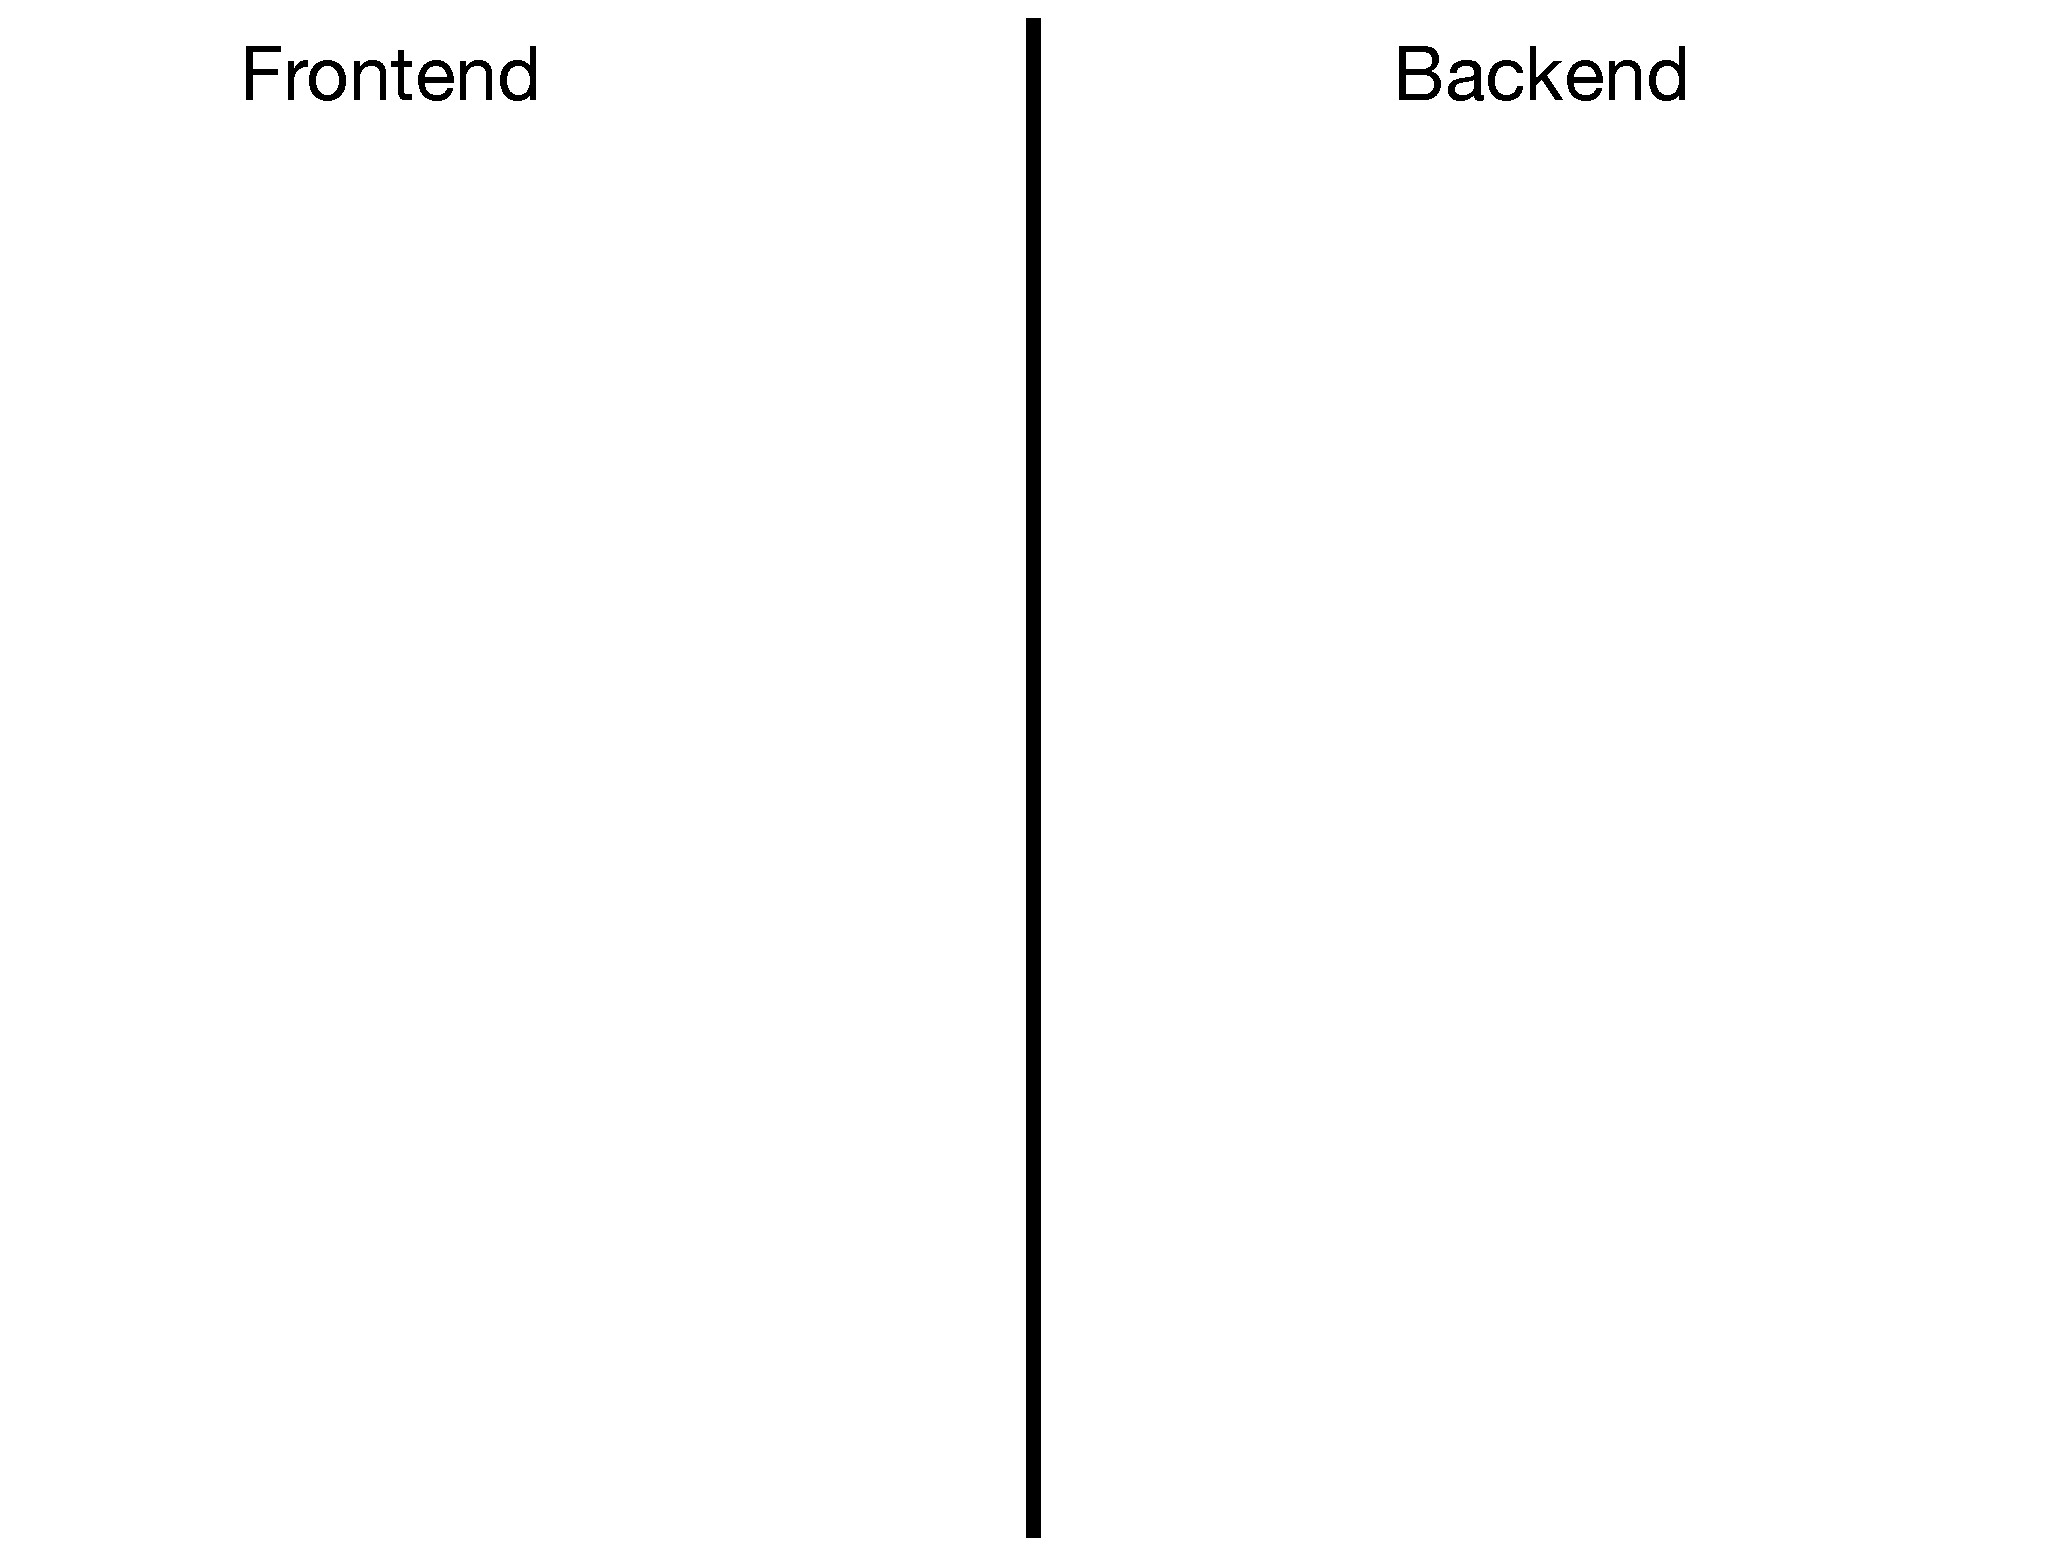
\includegraphics[width=\textwidth]{images/super-naive-approach-0.pdf}
}

\only<2>{
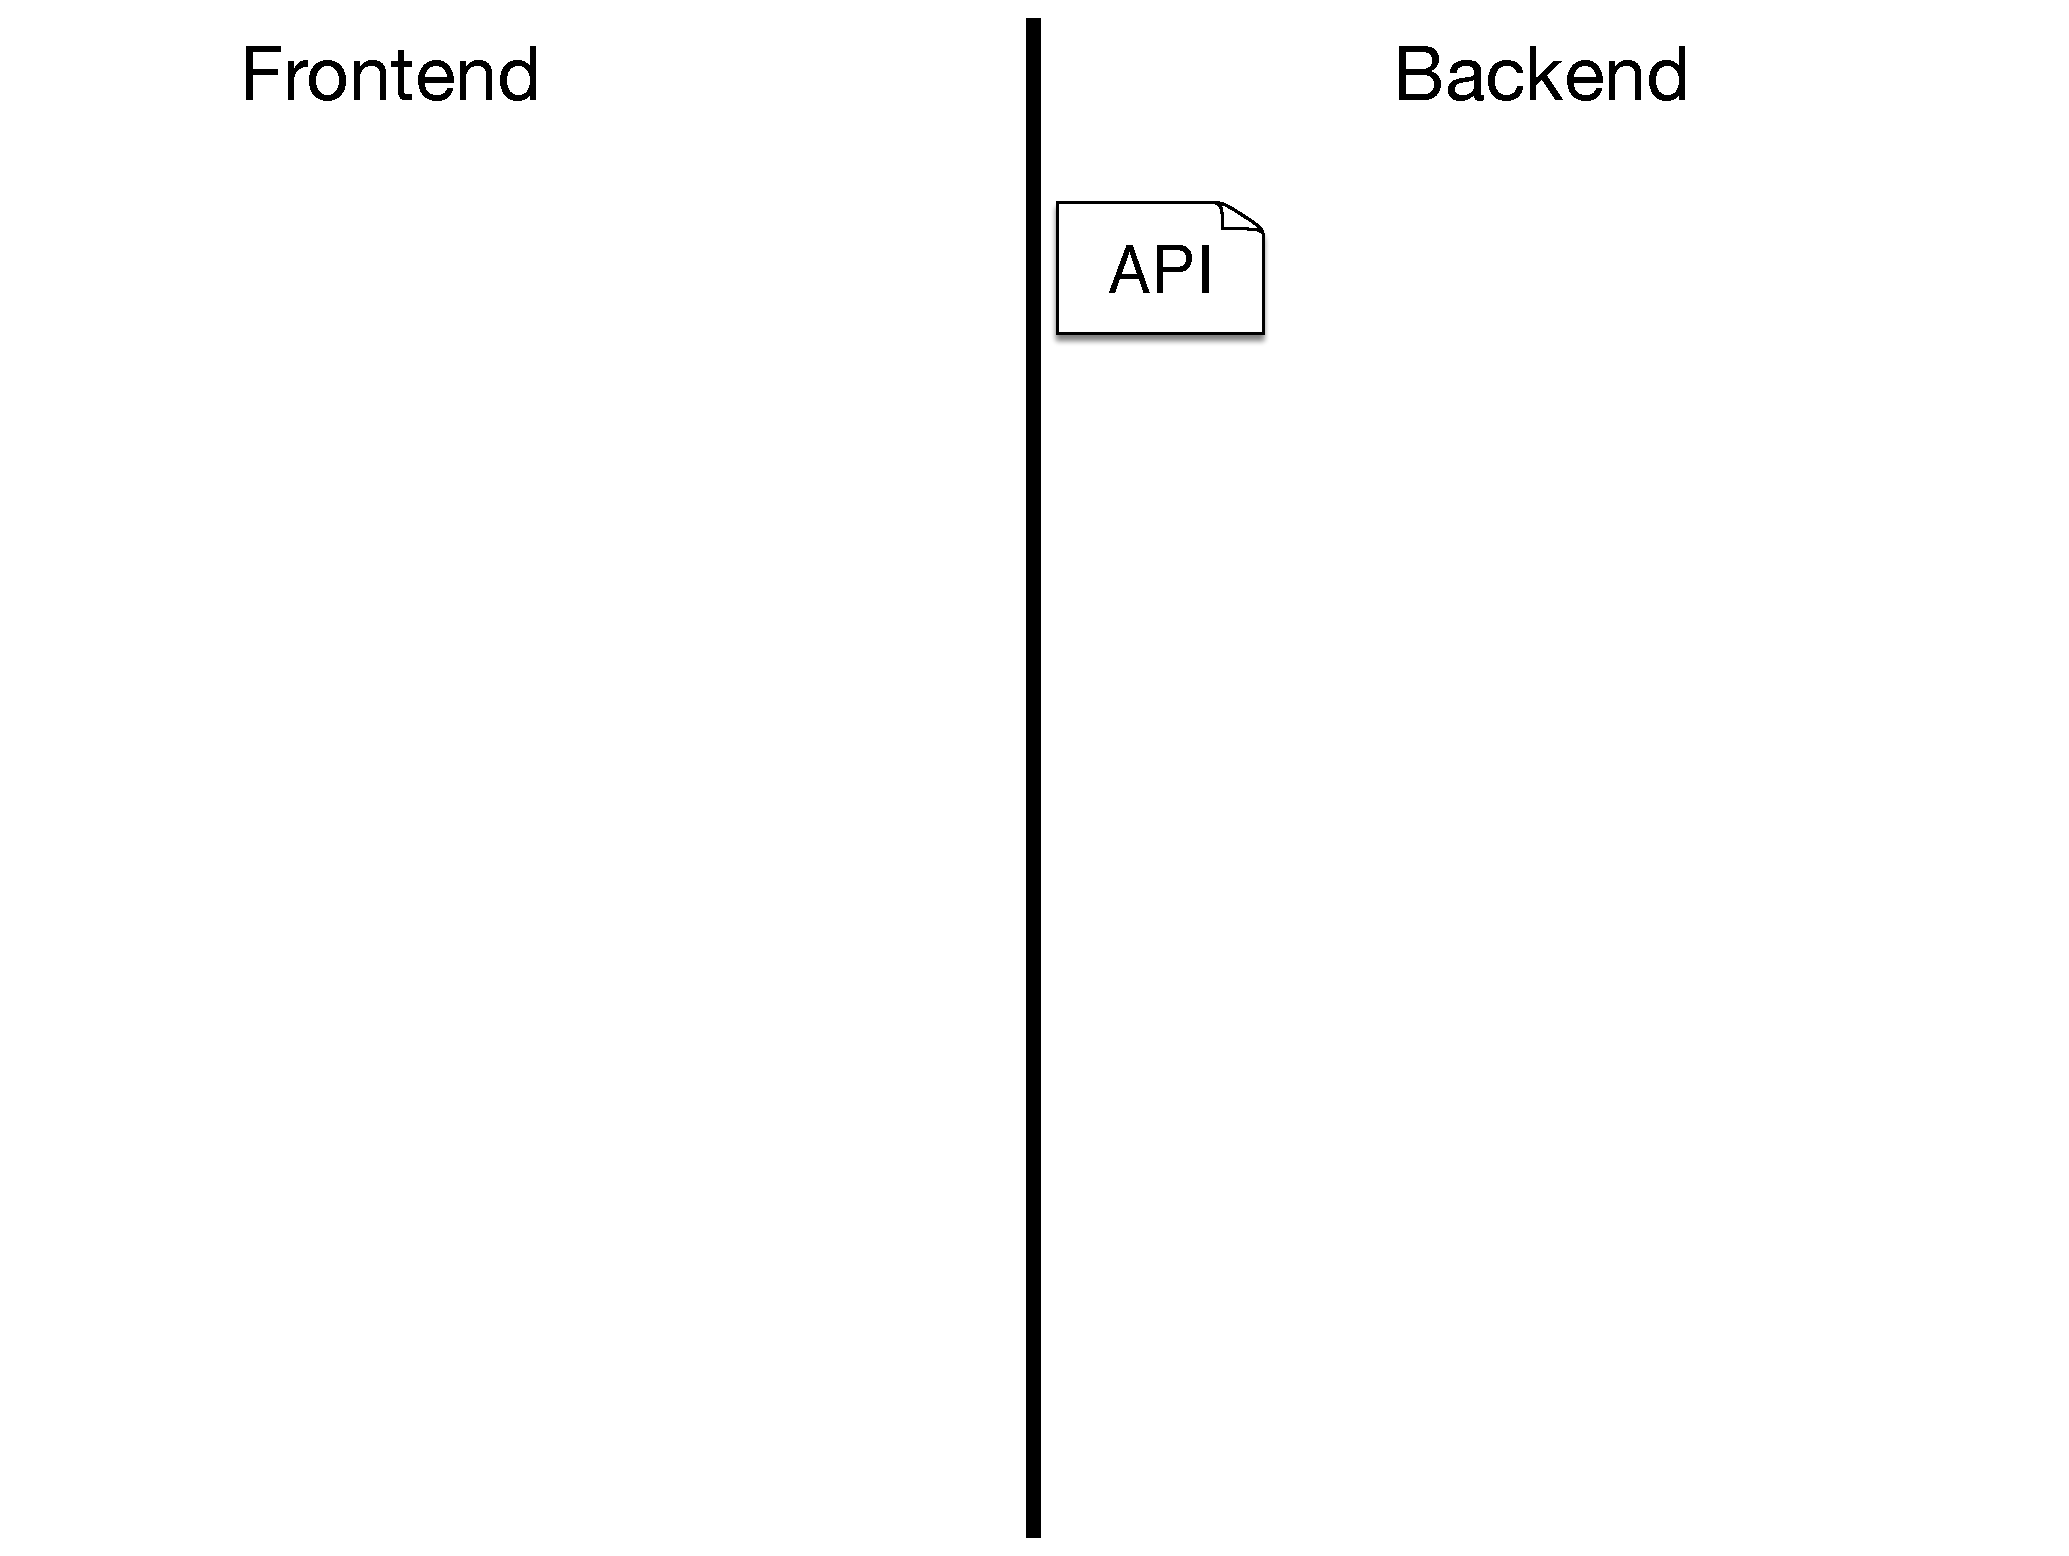
\includegraphics[width=\textwidth]{images/super-naive-approach-1.pdf}
}

\only<3>{
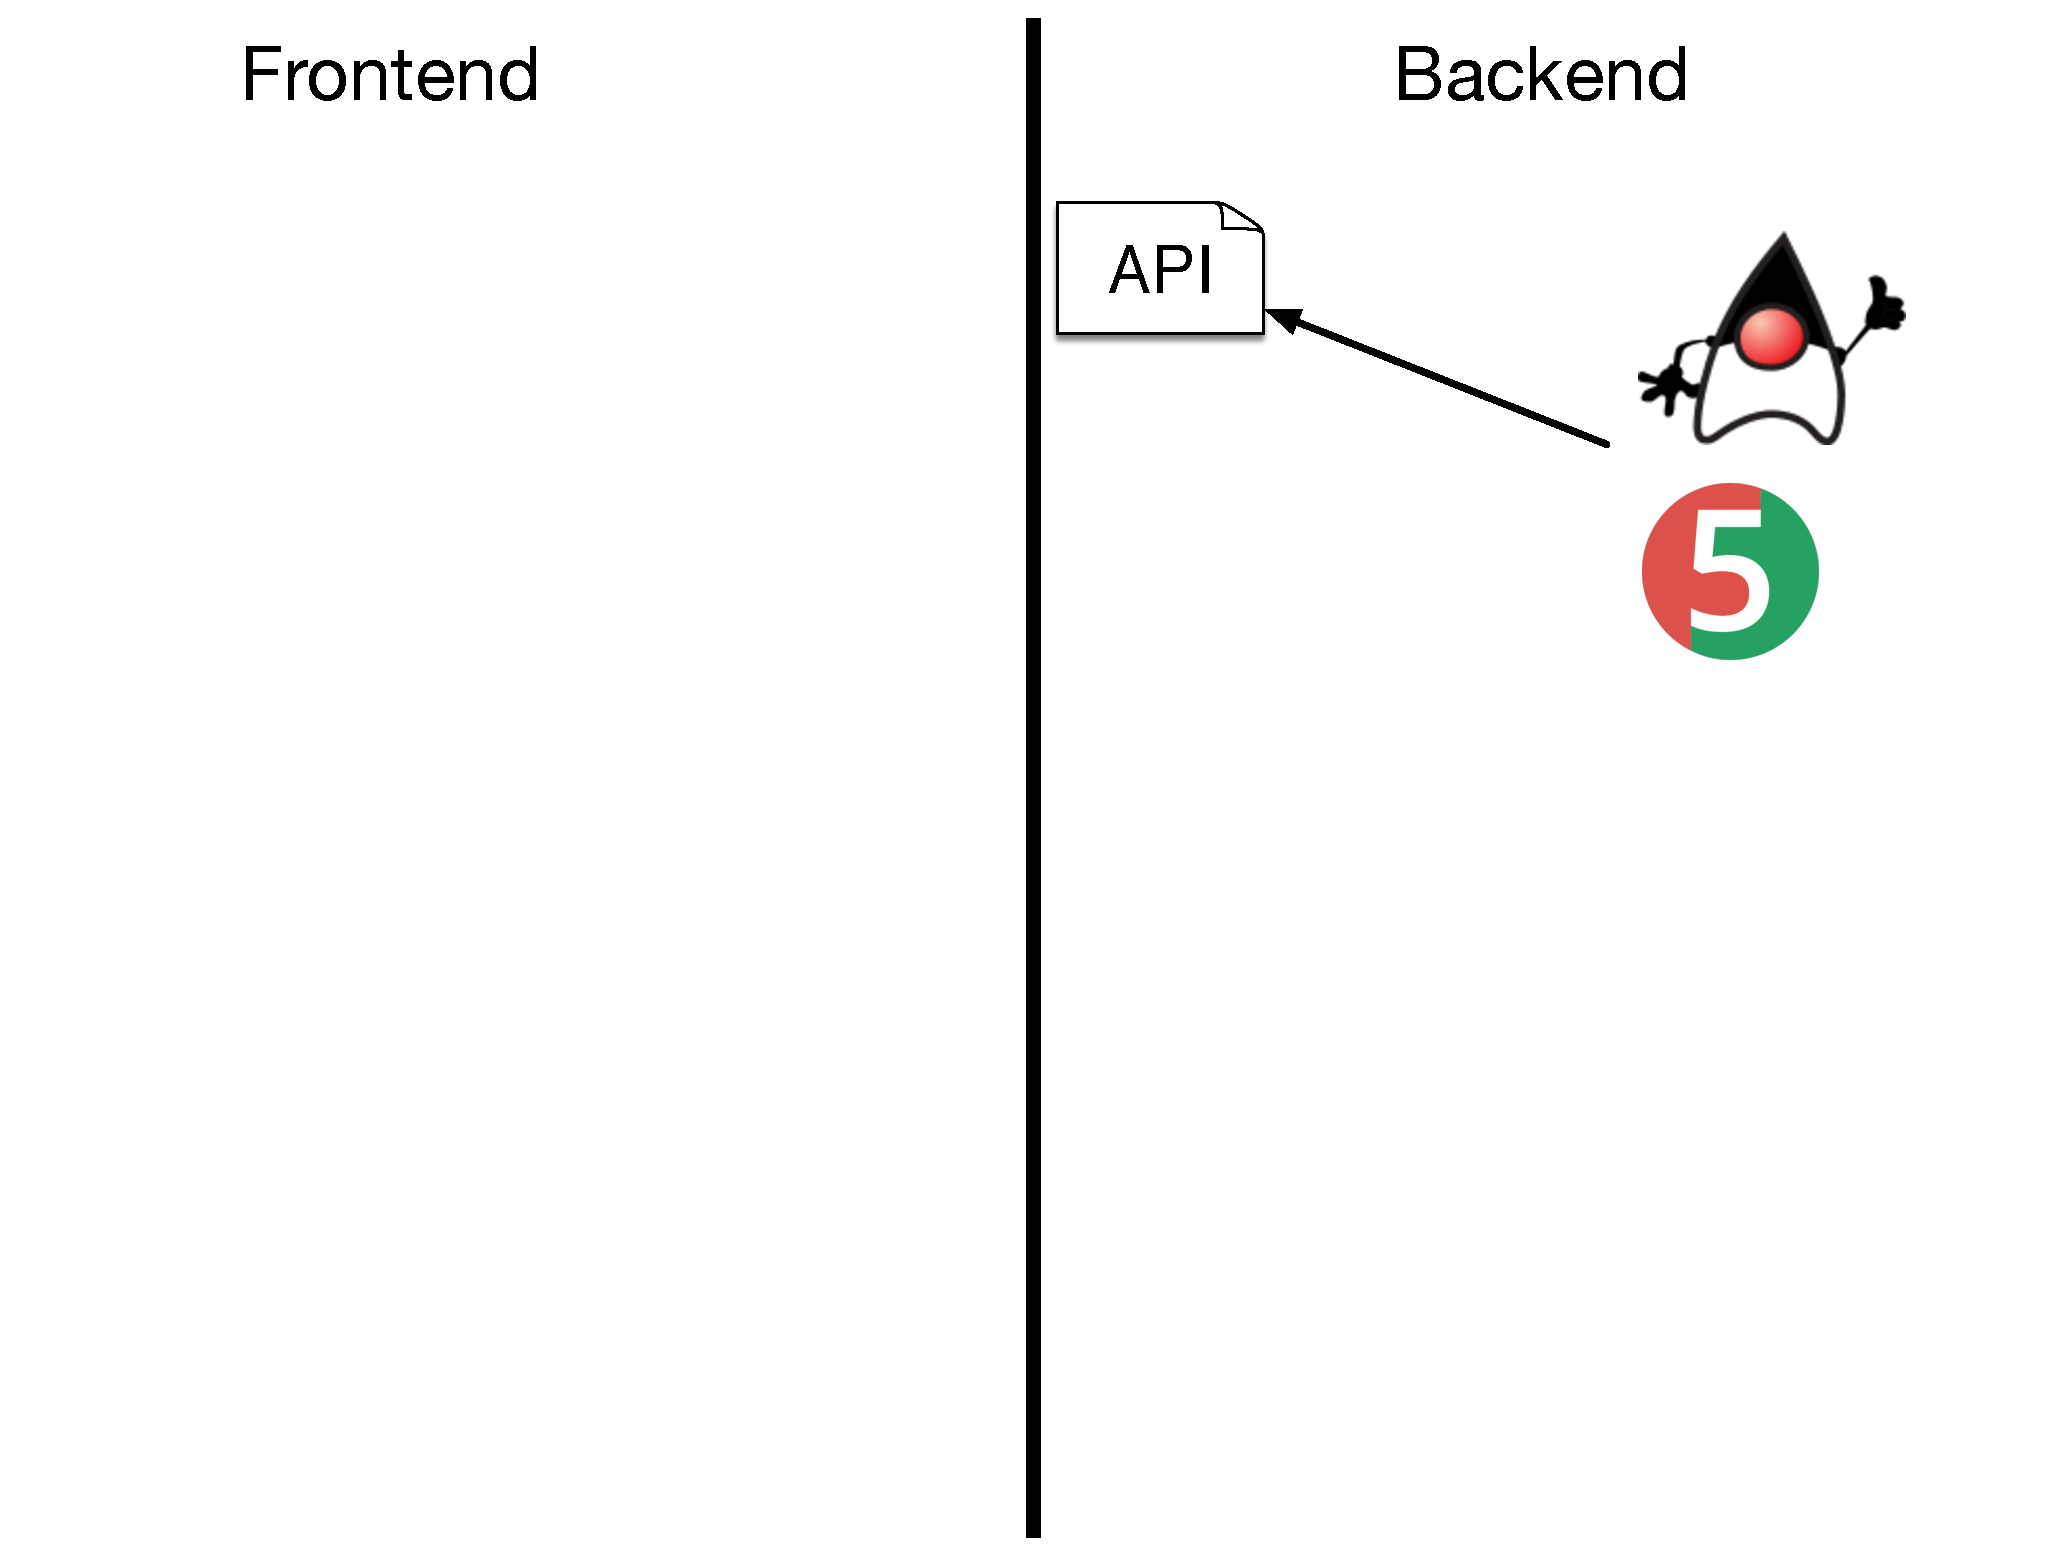
\includegraphics[width=\textwidth]{images/super-naive-approach-2.pdf}
}

\only<4>{
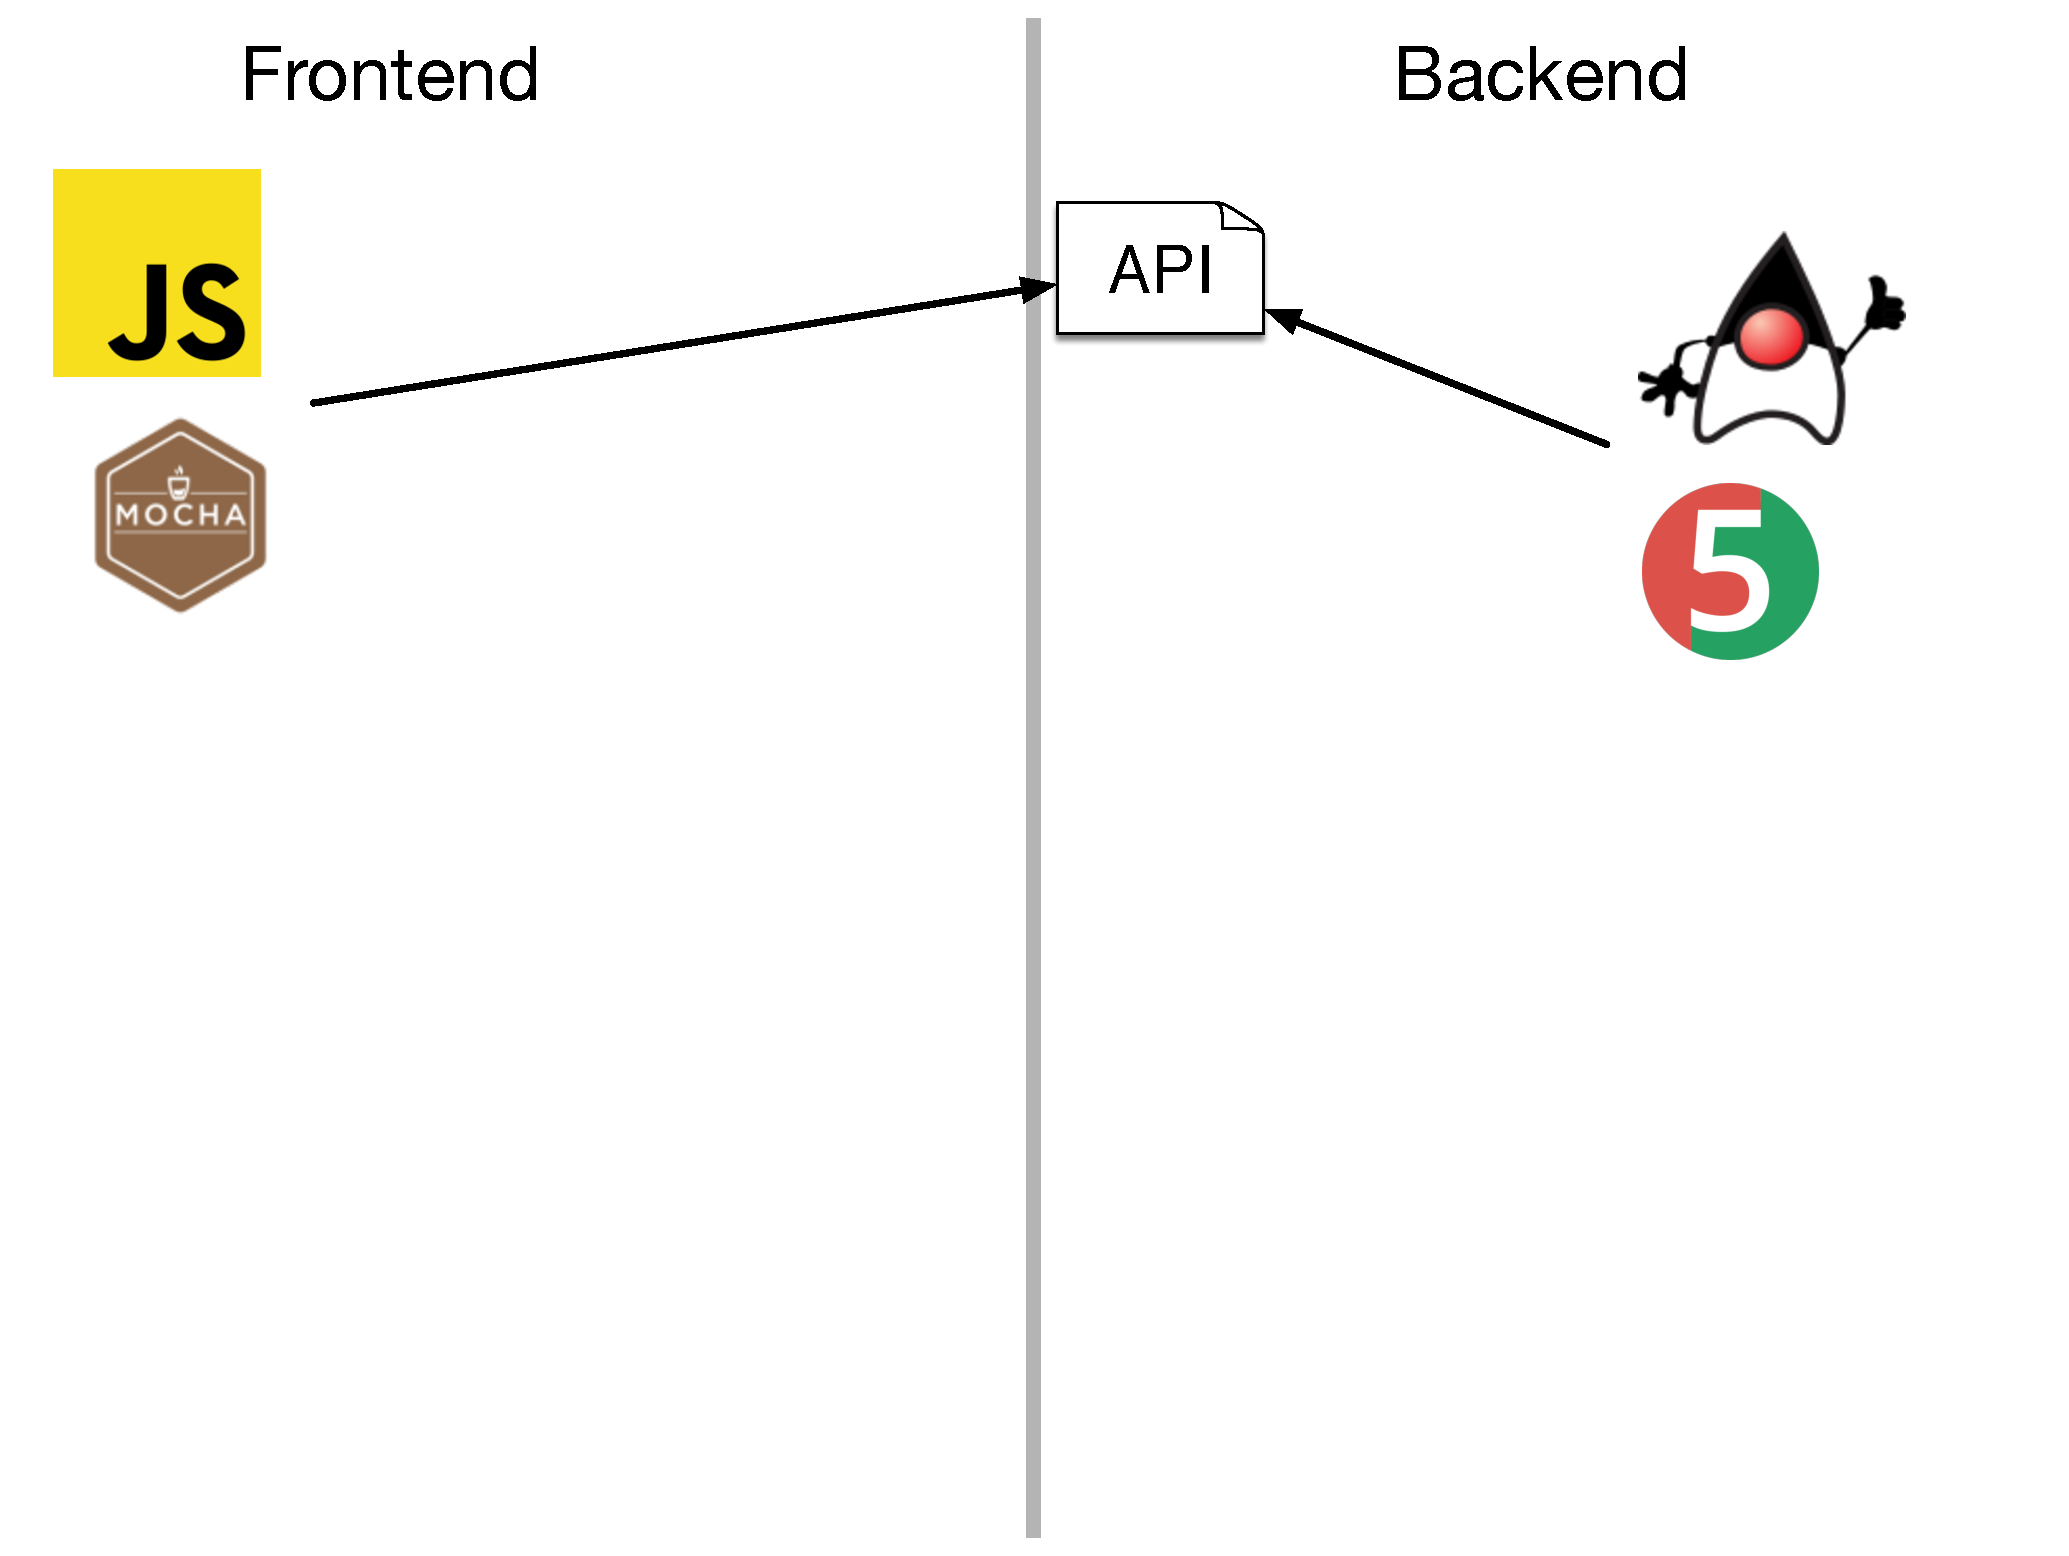
\includegraphics[width=\textwidth]{images/super-naive-approach-3.pdf}
}

\only<5>{
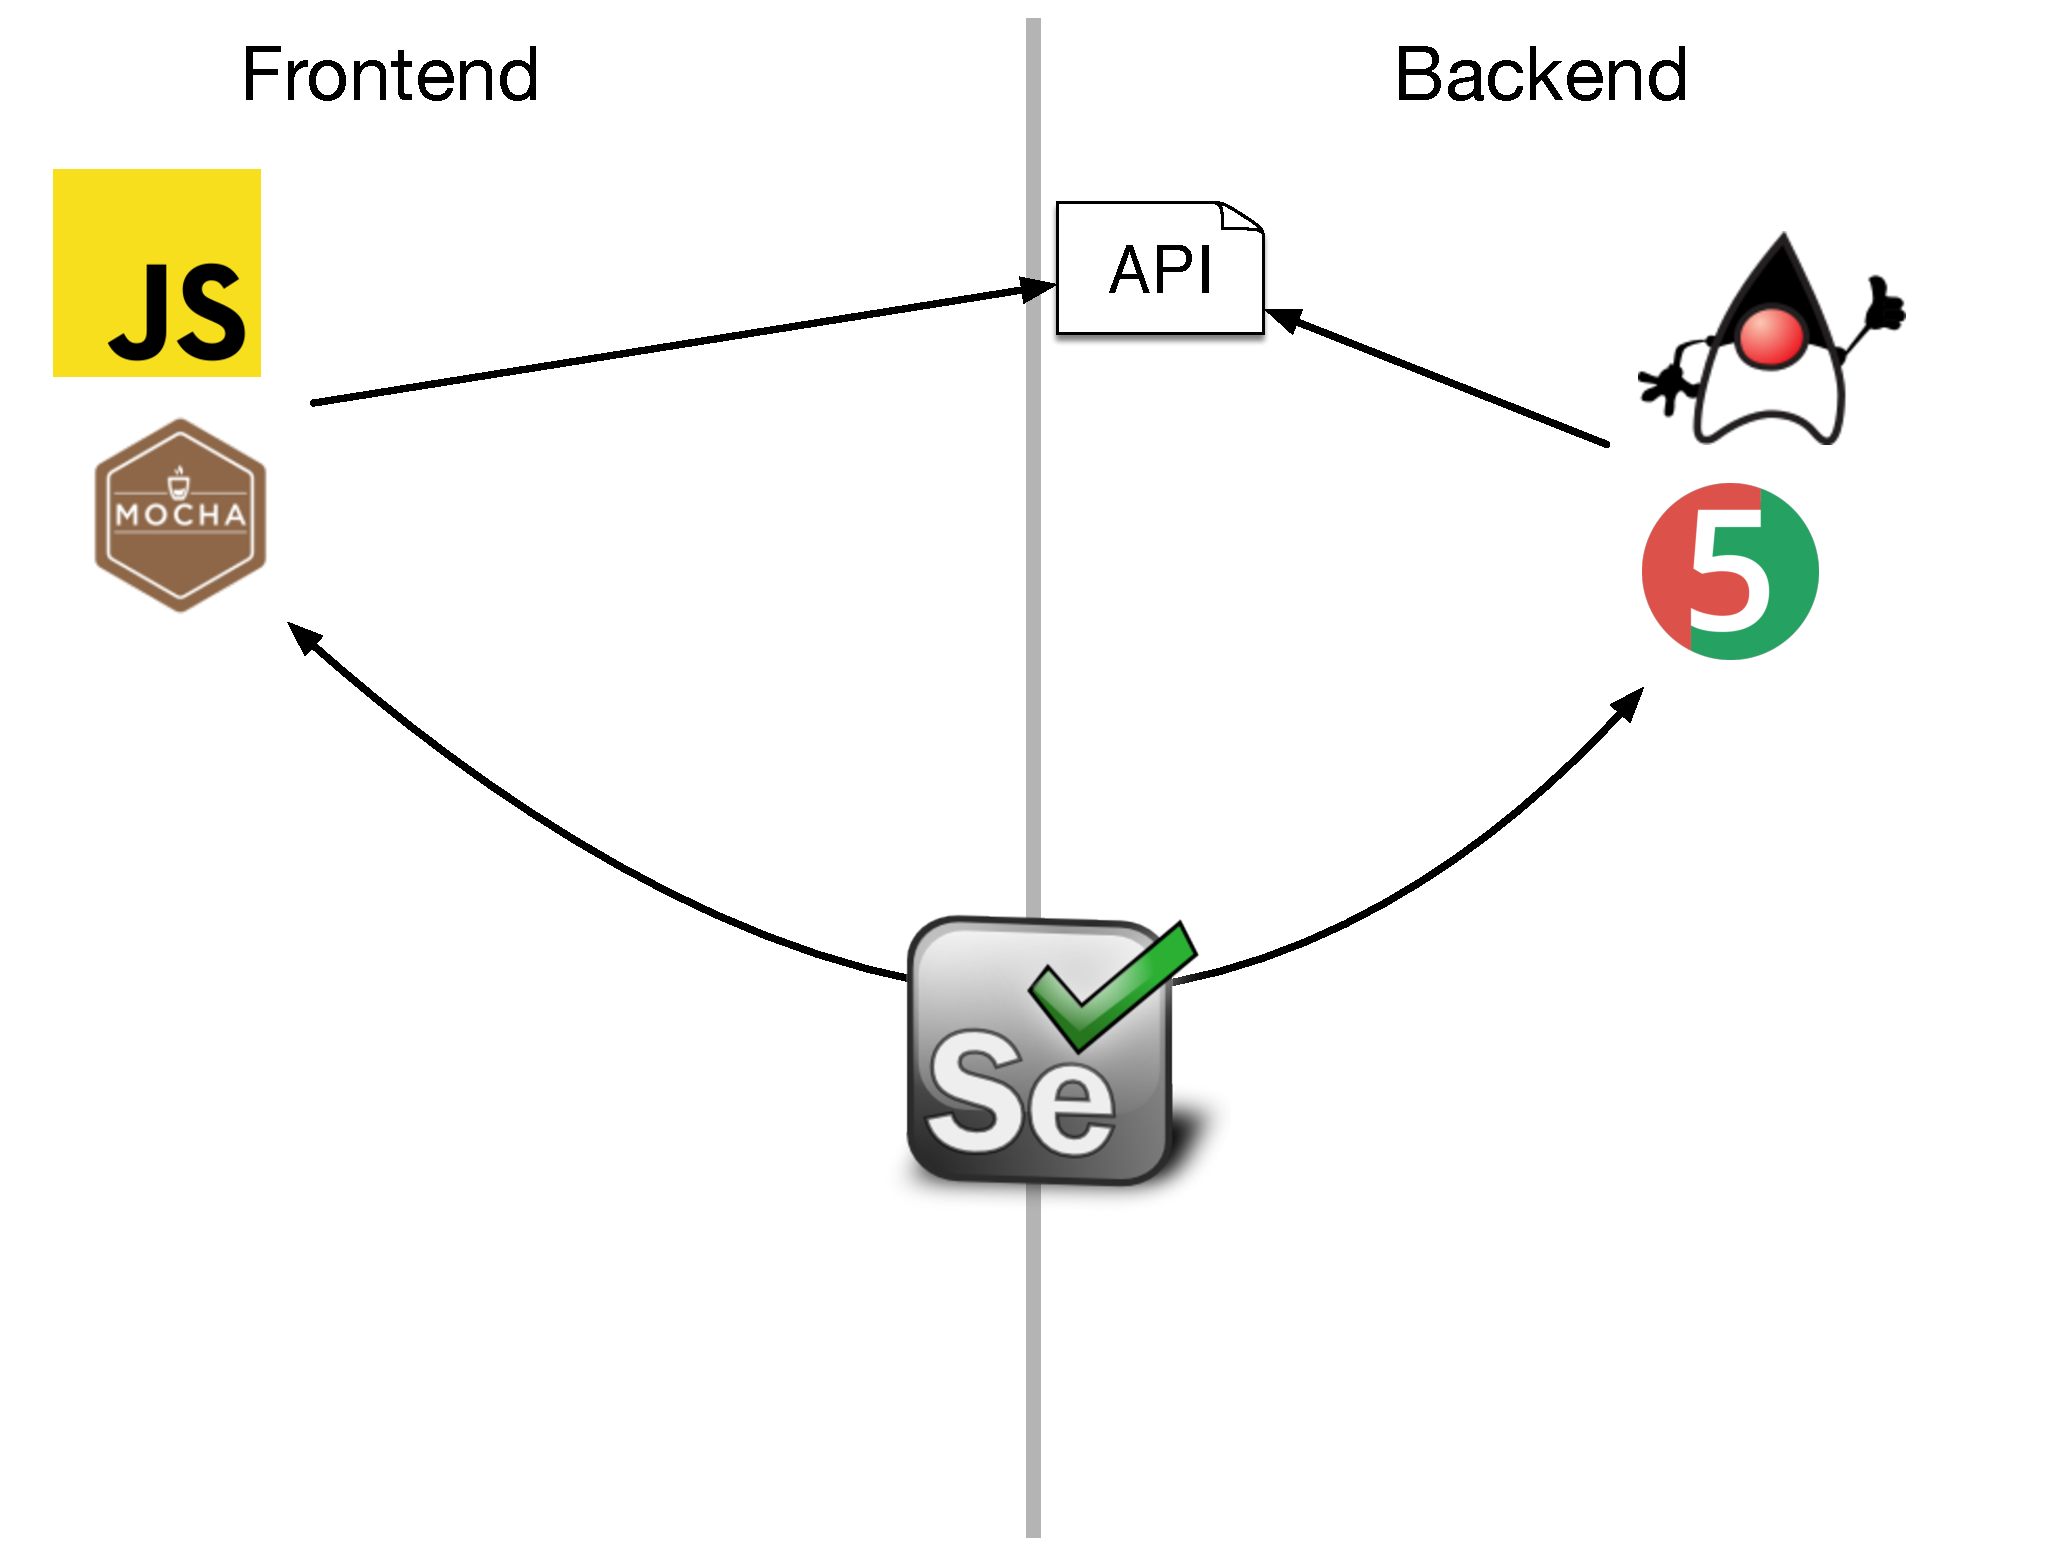
\includegraphics[width=\textwidth]{images/super-naive-approach-4.pdf}
}

\end{frame}

\begin{frame}[fragile]{}

\begin{center}
{\Huge
But $\ldots$
}
\end{center}

\end{frame}

\begin{frame}[fragile]{}

\only<1>{
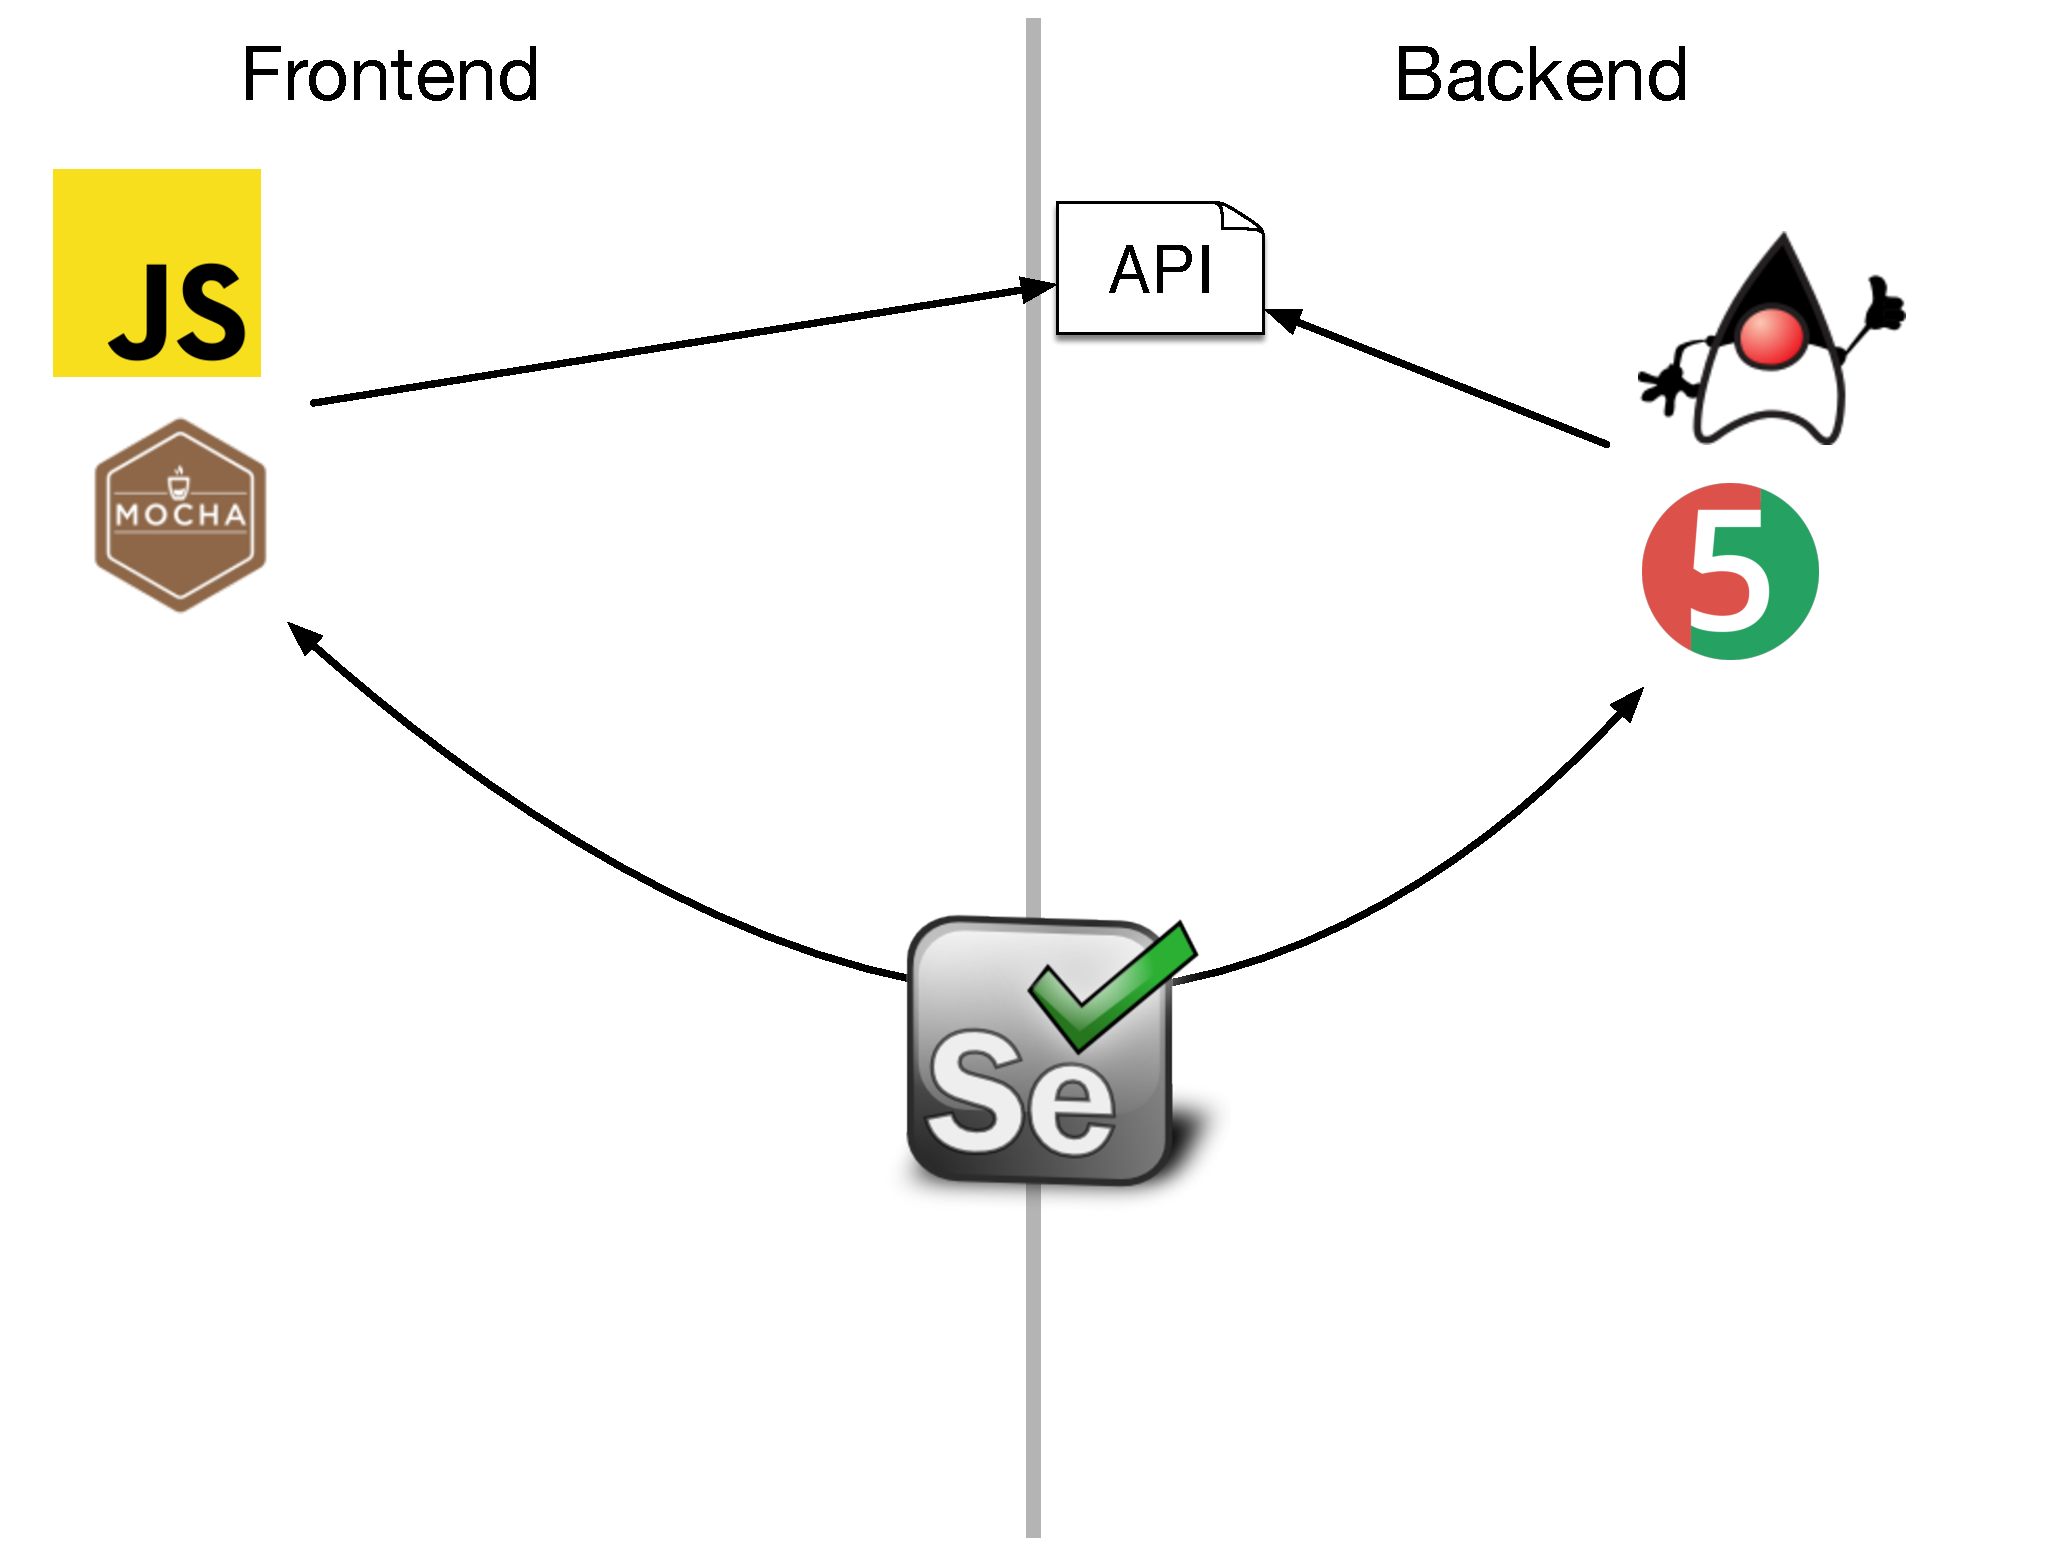
\includegraphics[width=\textwidth]{images/super-naive-approach-4.pdf}
}

\only<2>{
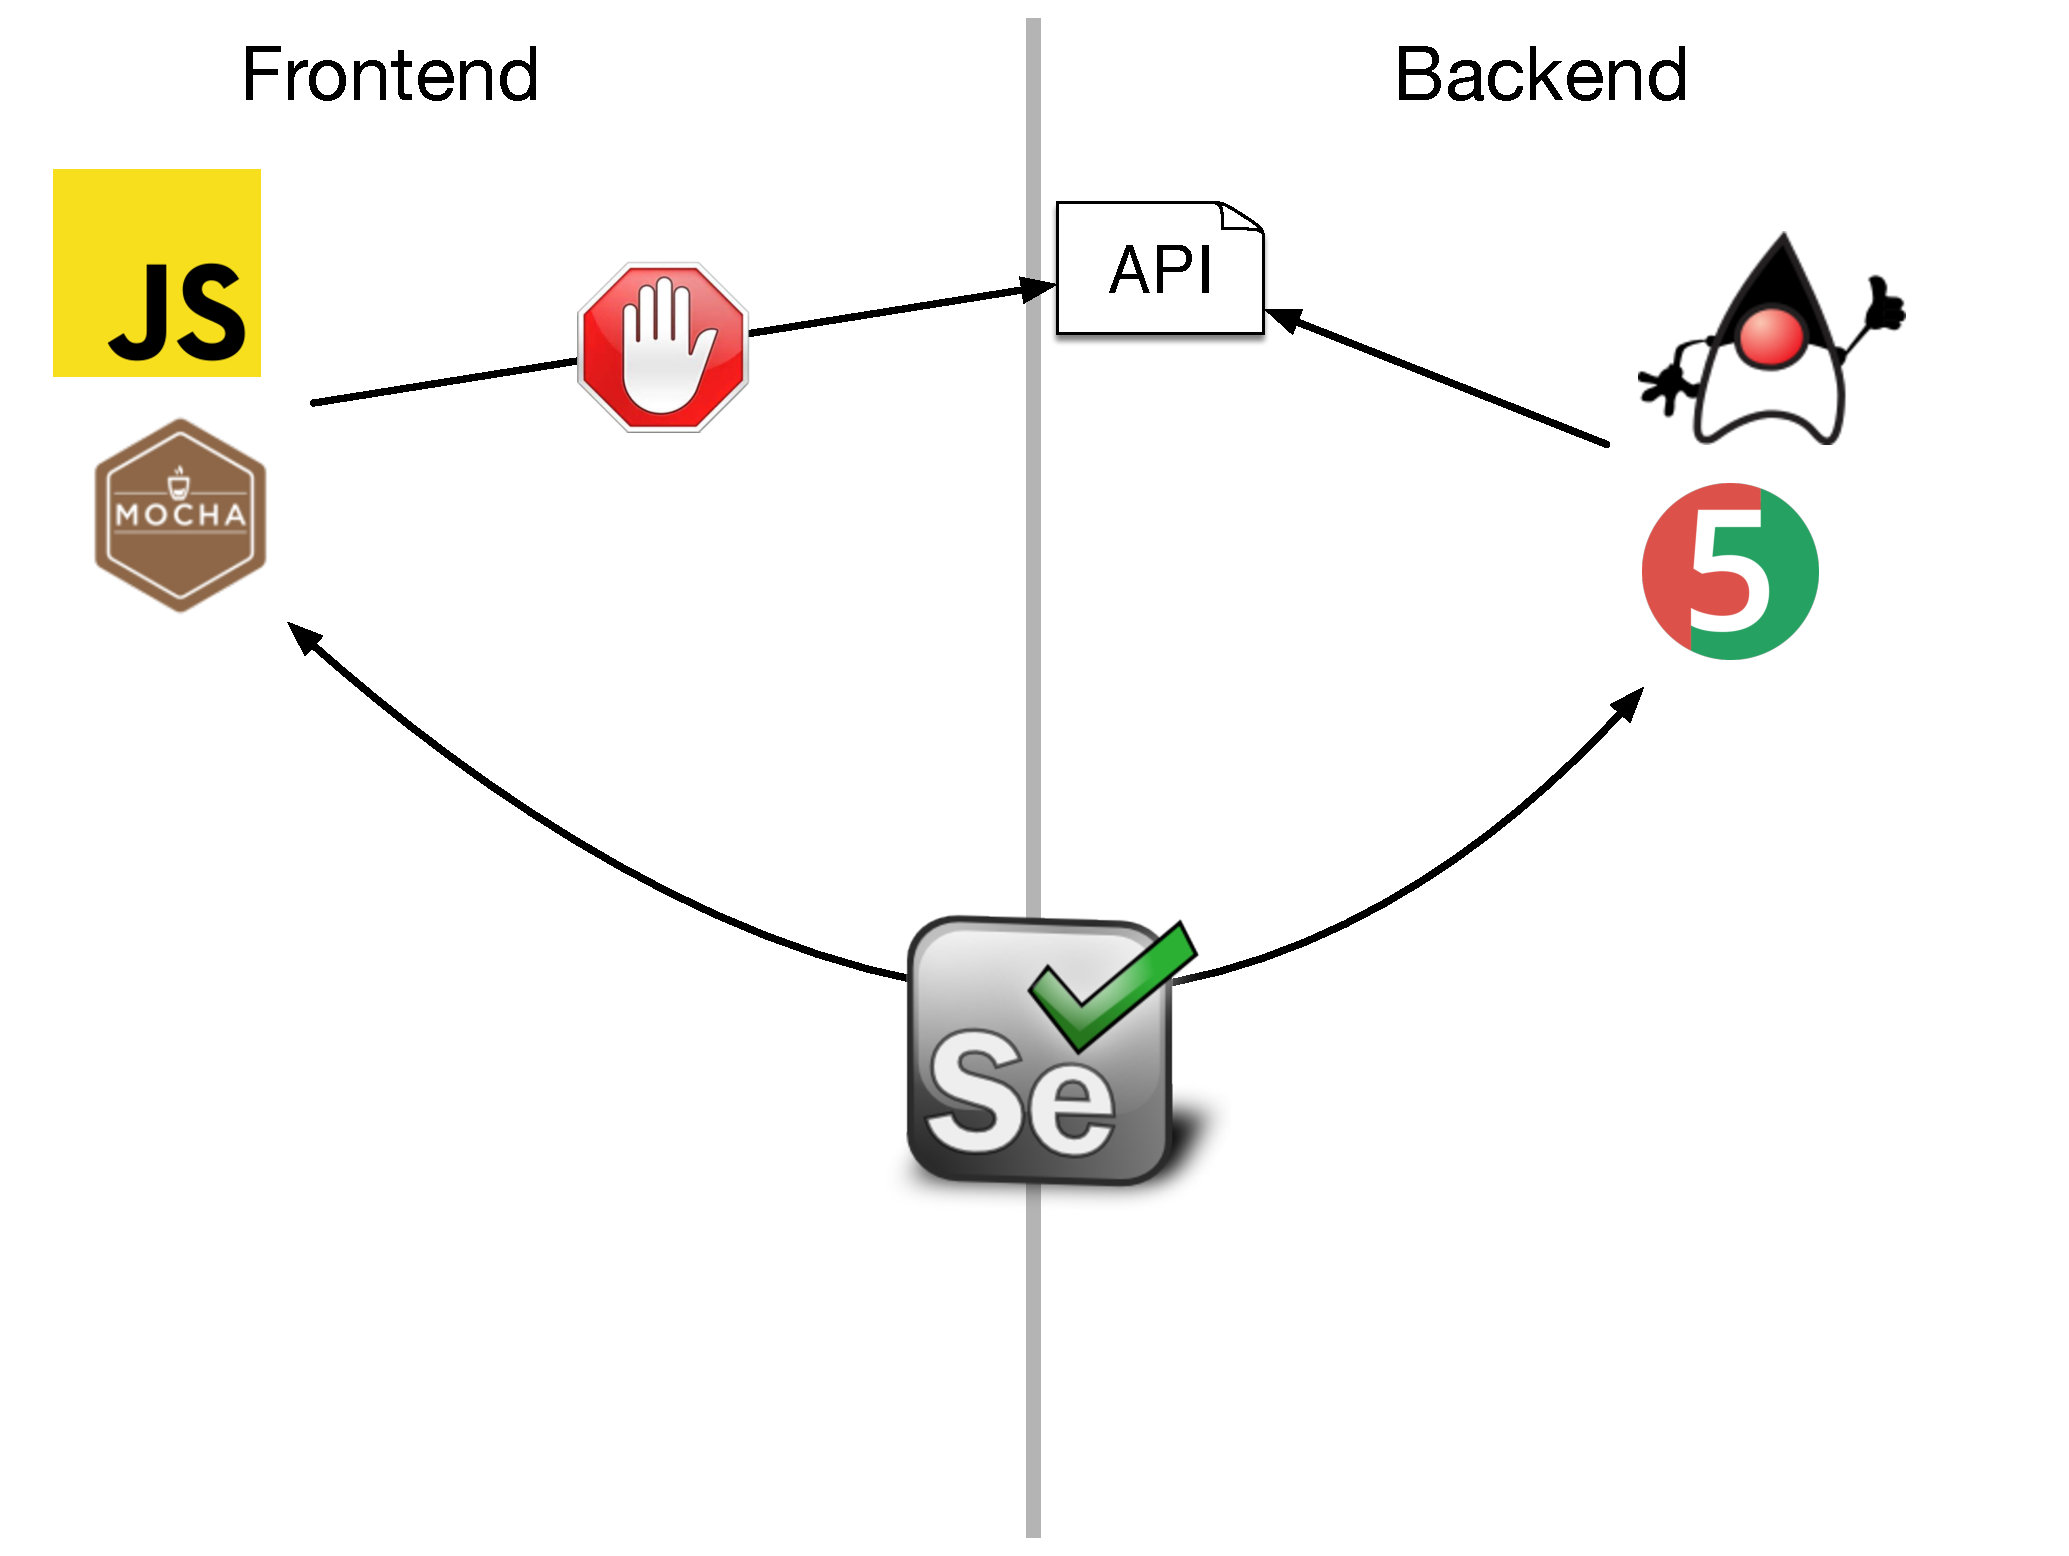
\includegraphics[width=\textwidth]{images/super-naive-approach-5.pdf}
}

\only<3>{
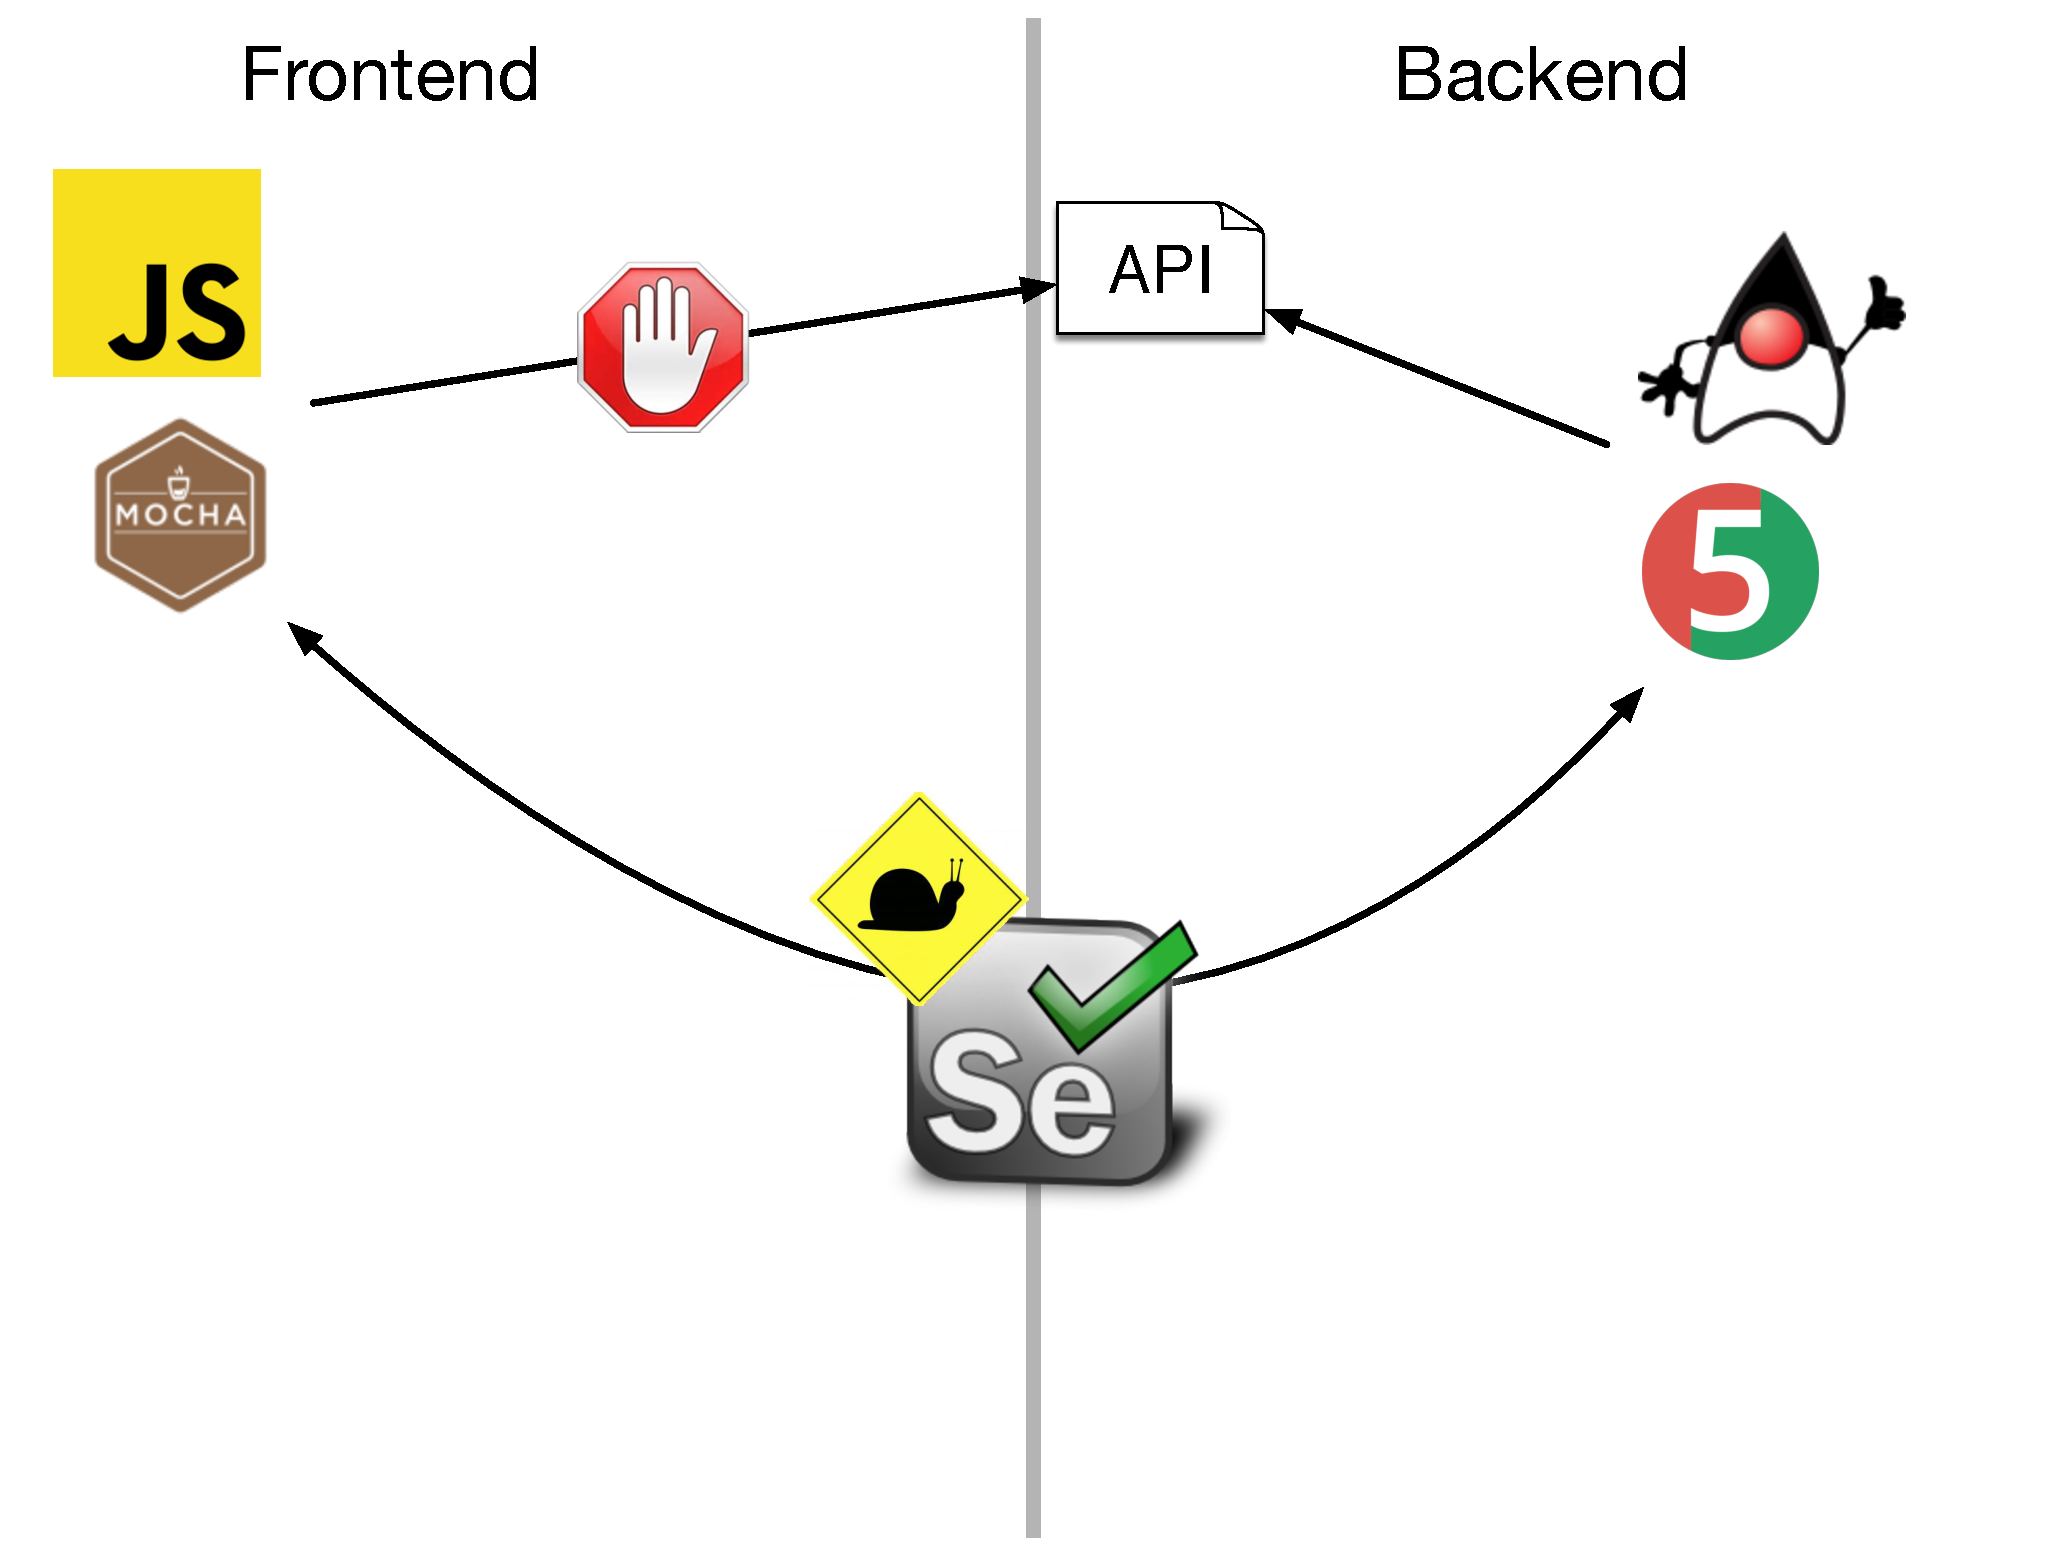
\includegraphics[width=\textwidth]{images/super-naive-approach-6.pdf}
}

\only<4>{
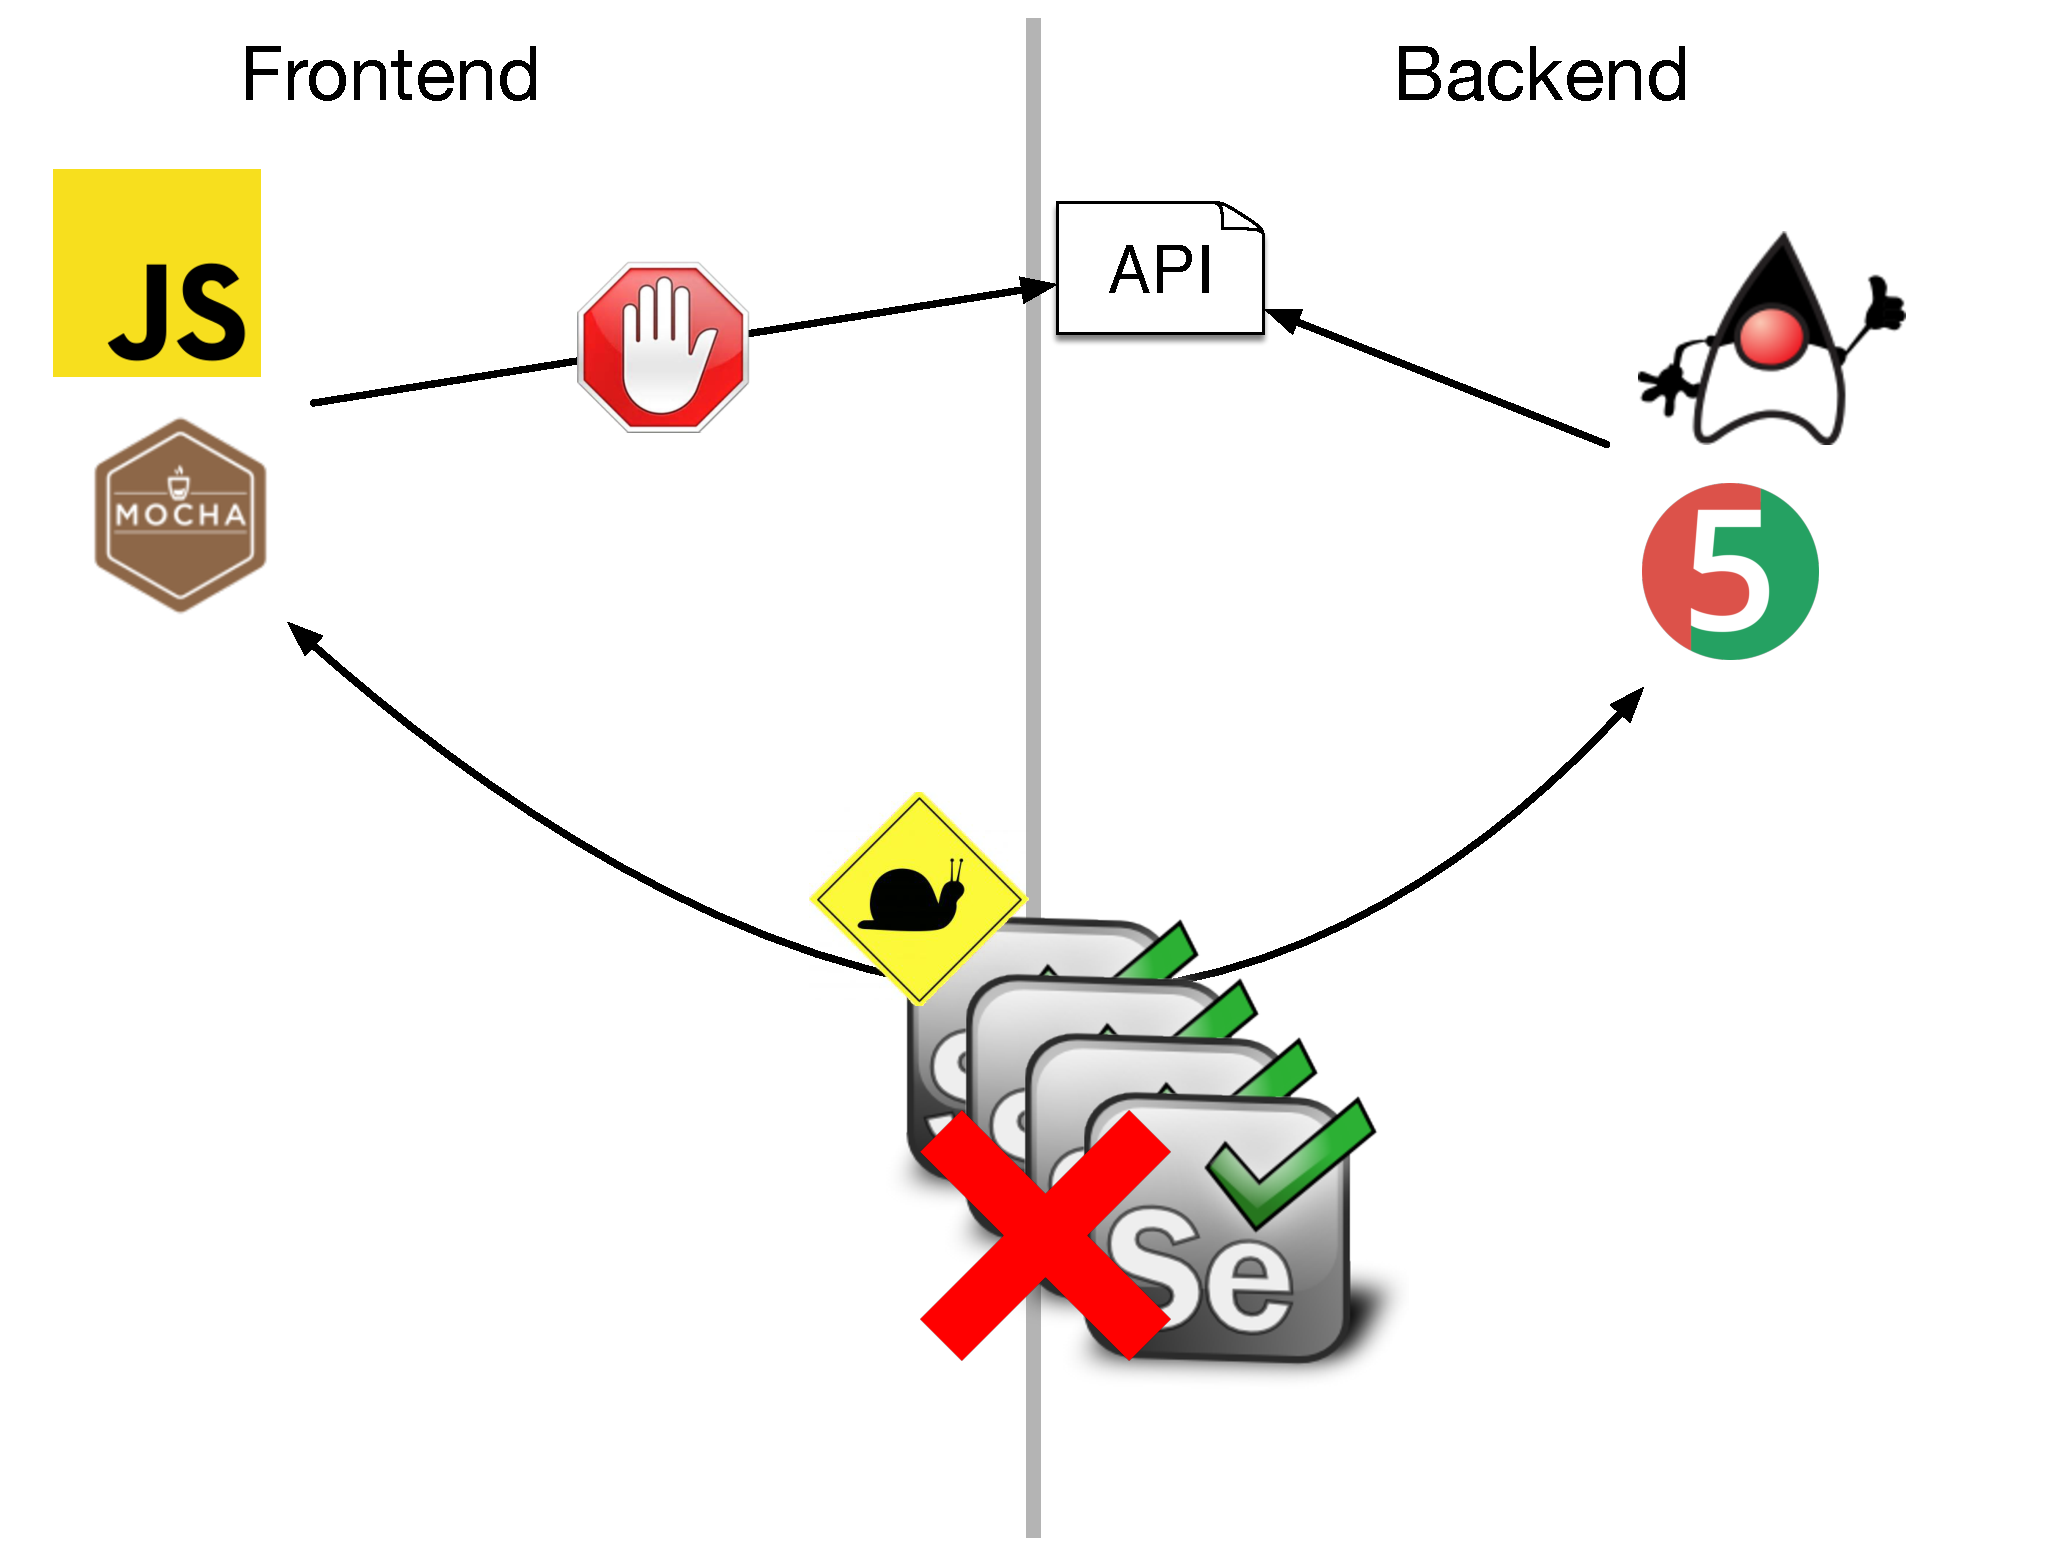
\includegraphics[width=\textwidth]{images/super-naive-approach-7.pdf}
}

\end{frame}


%%%%%%%%%%%%%%%%%%%%%%%%%%%%%%%%%%%%%%%%%%%%%%%%%%
\begin{frame}[fragile]{}

\begin{center}
{\Huge
``Still Quite Na\"ive'' Approach
}
\end{center}

\end{frame}

\begin{frame}[fragile]{}

\only<1>{
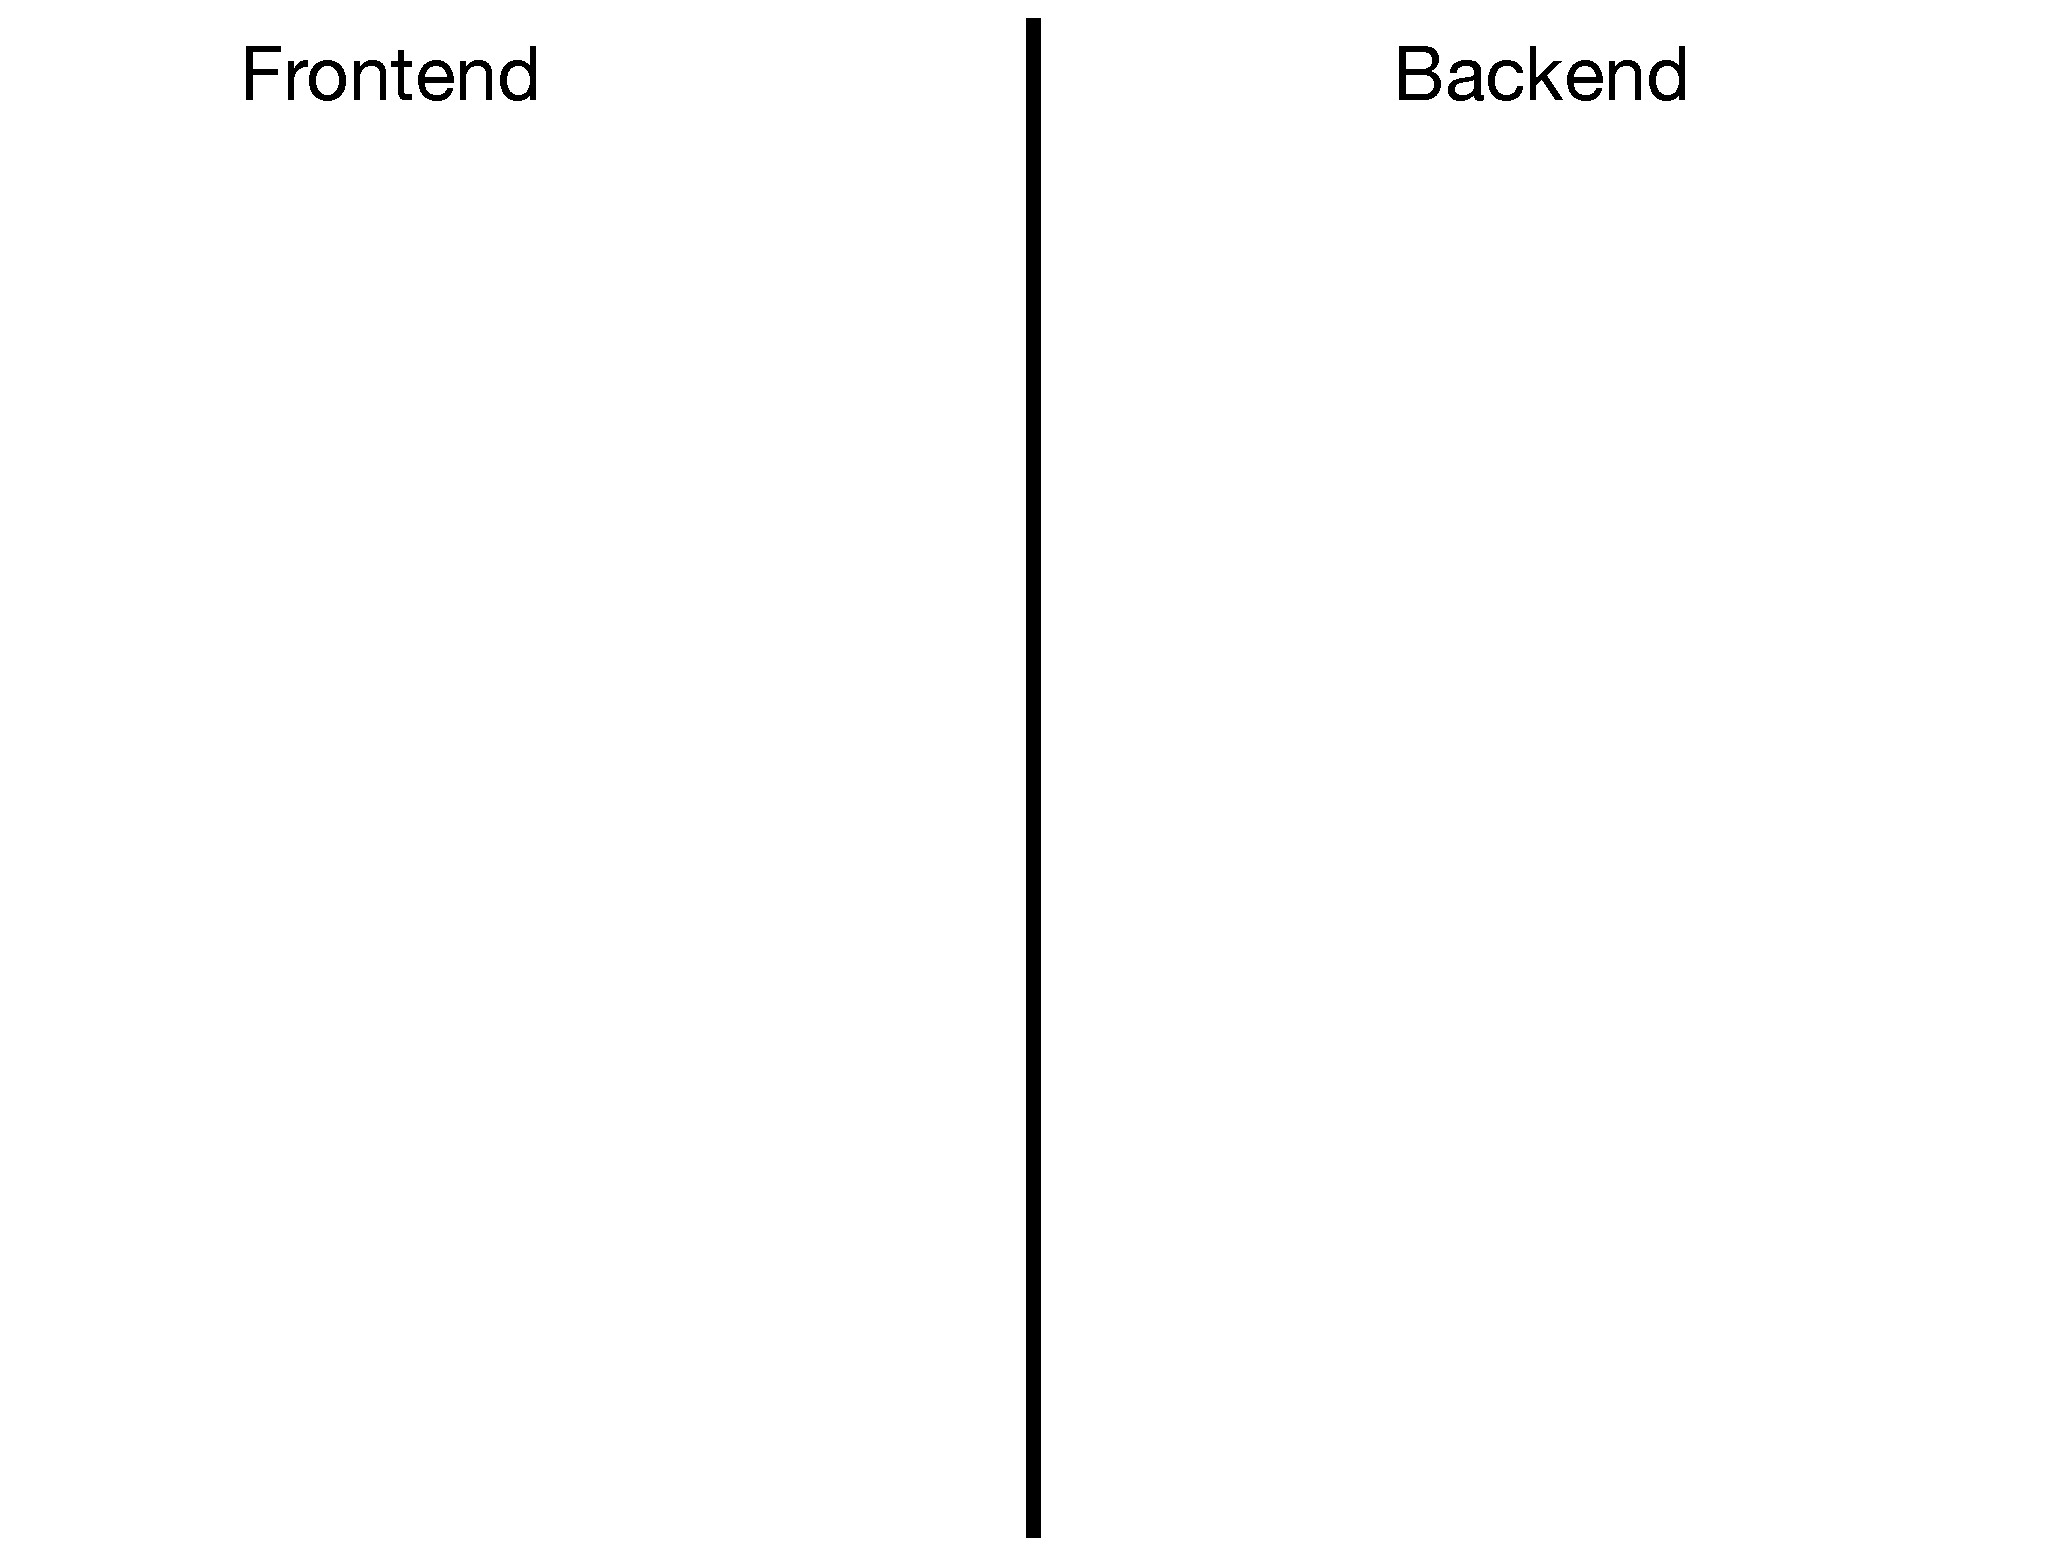
\includegraphics[width=\textwidth]{images/still-quite-naive-approach-0.pdf}
}

\only<2>{
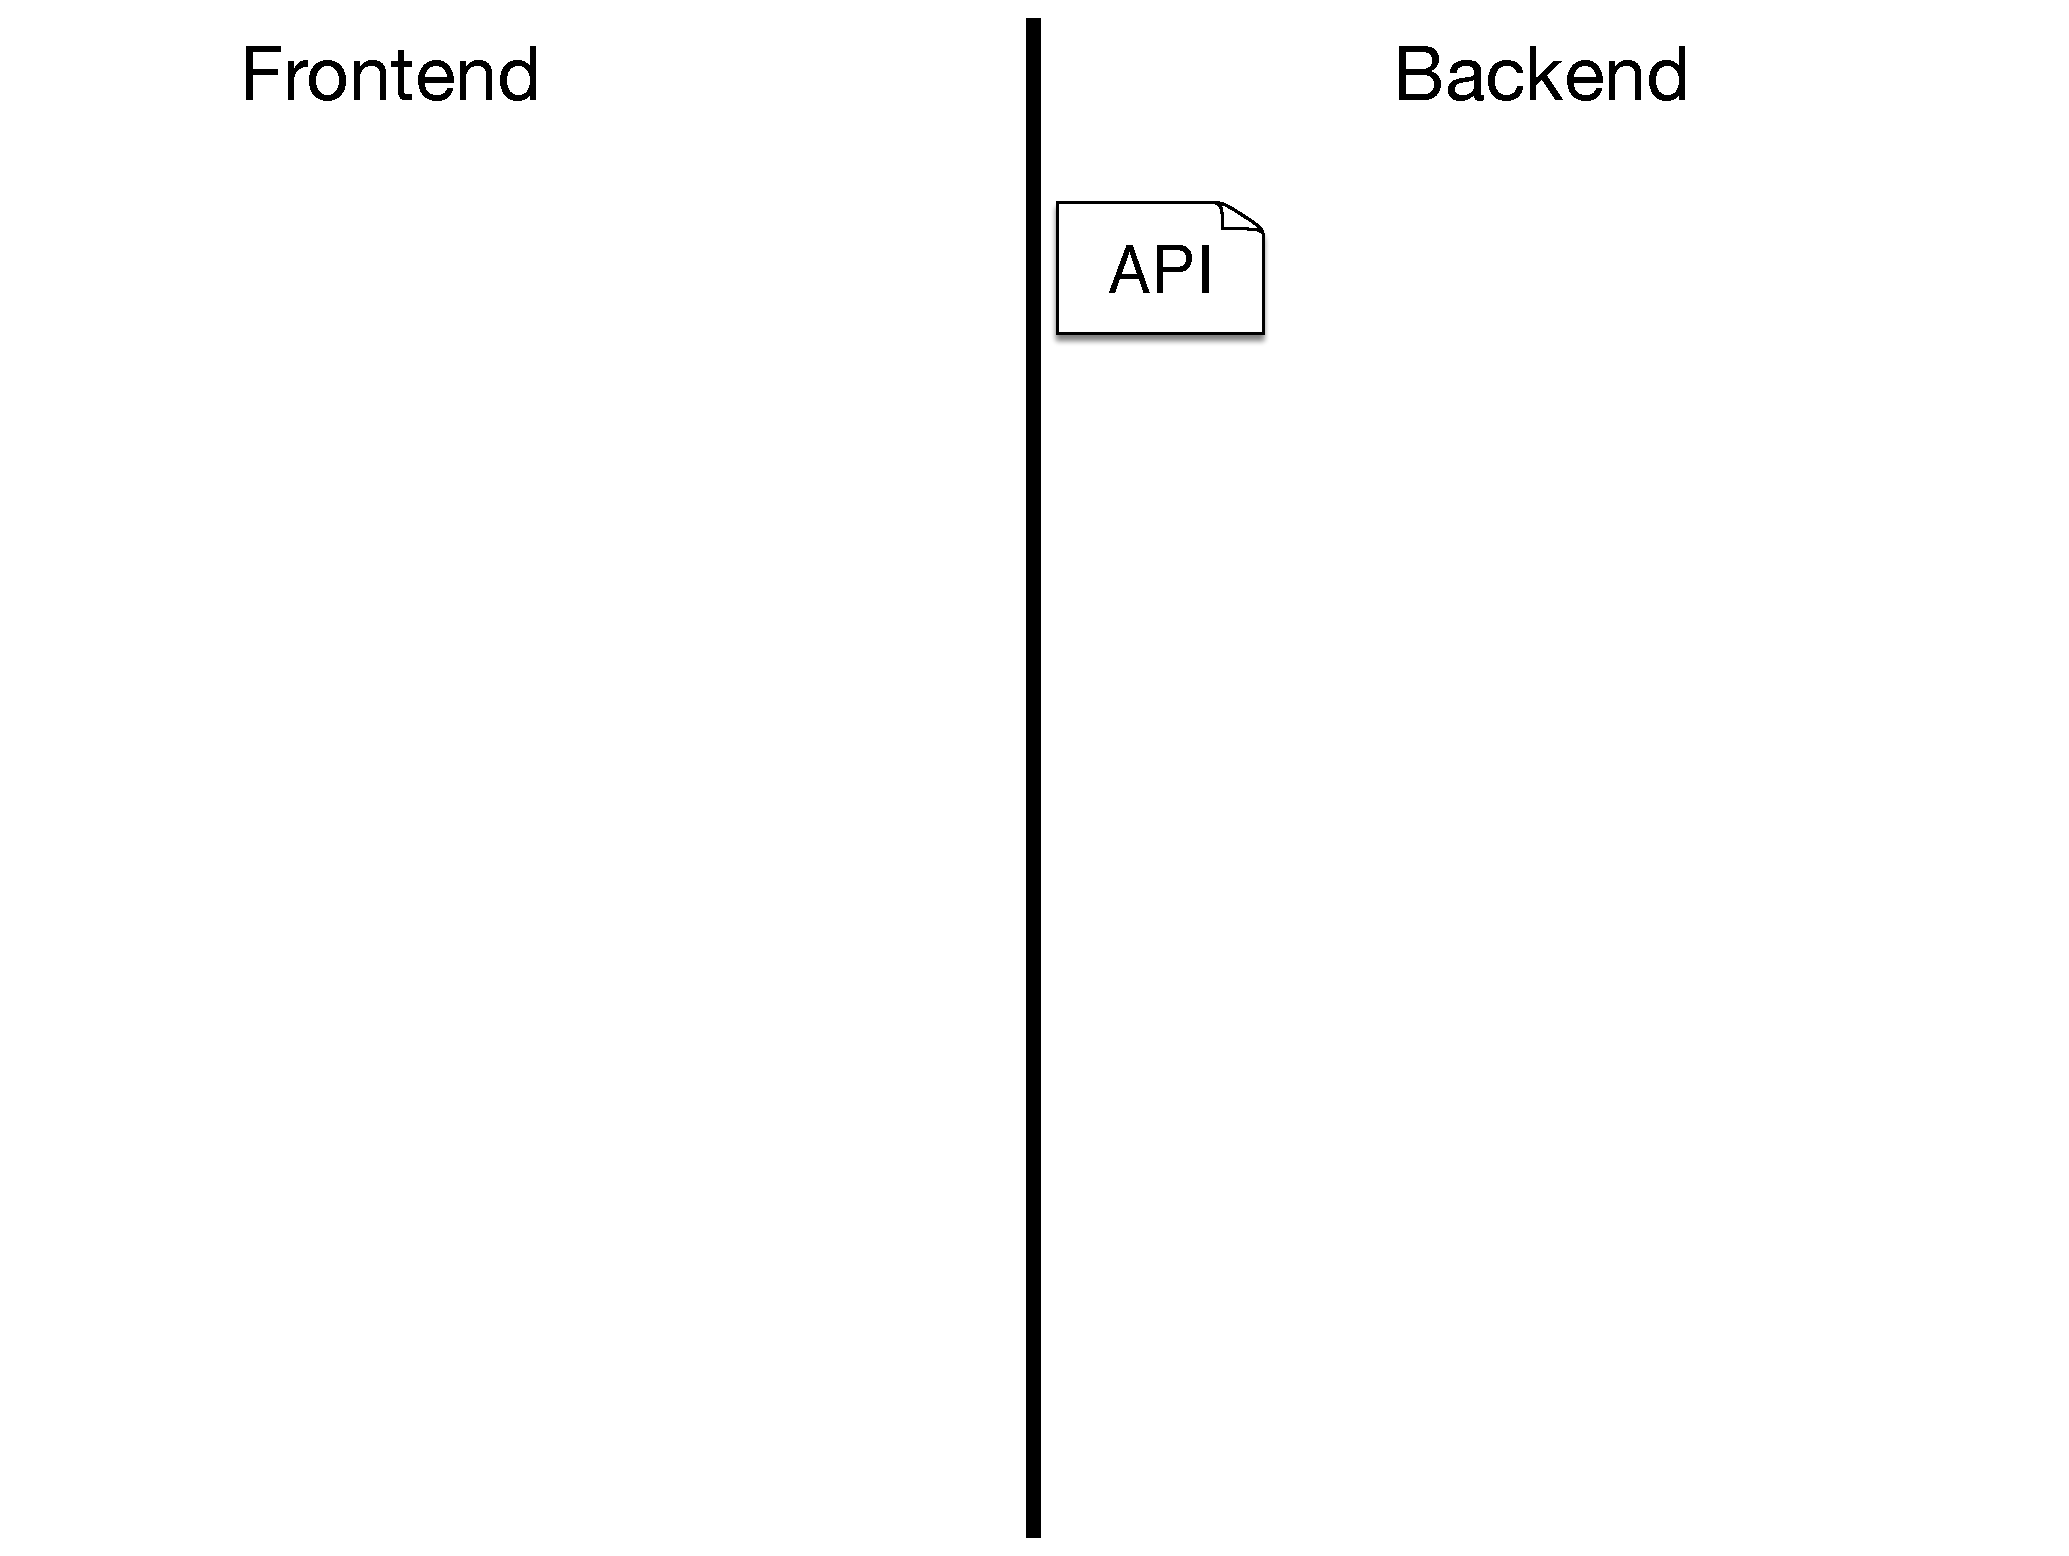
\includegraphics[width=\textwidth]{images/still-quite-naive-approach-1.pdf}
}

\only<3>{
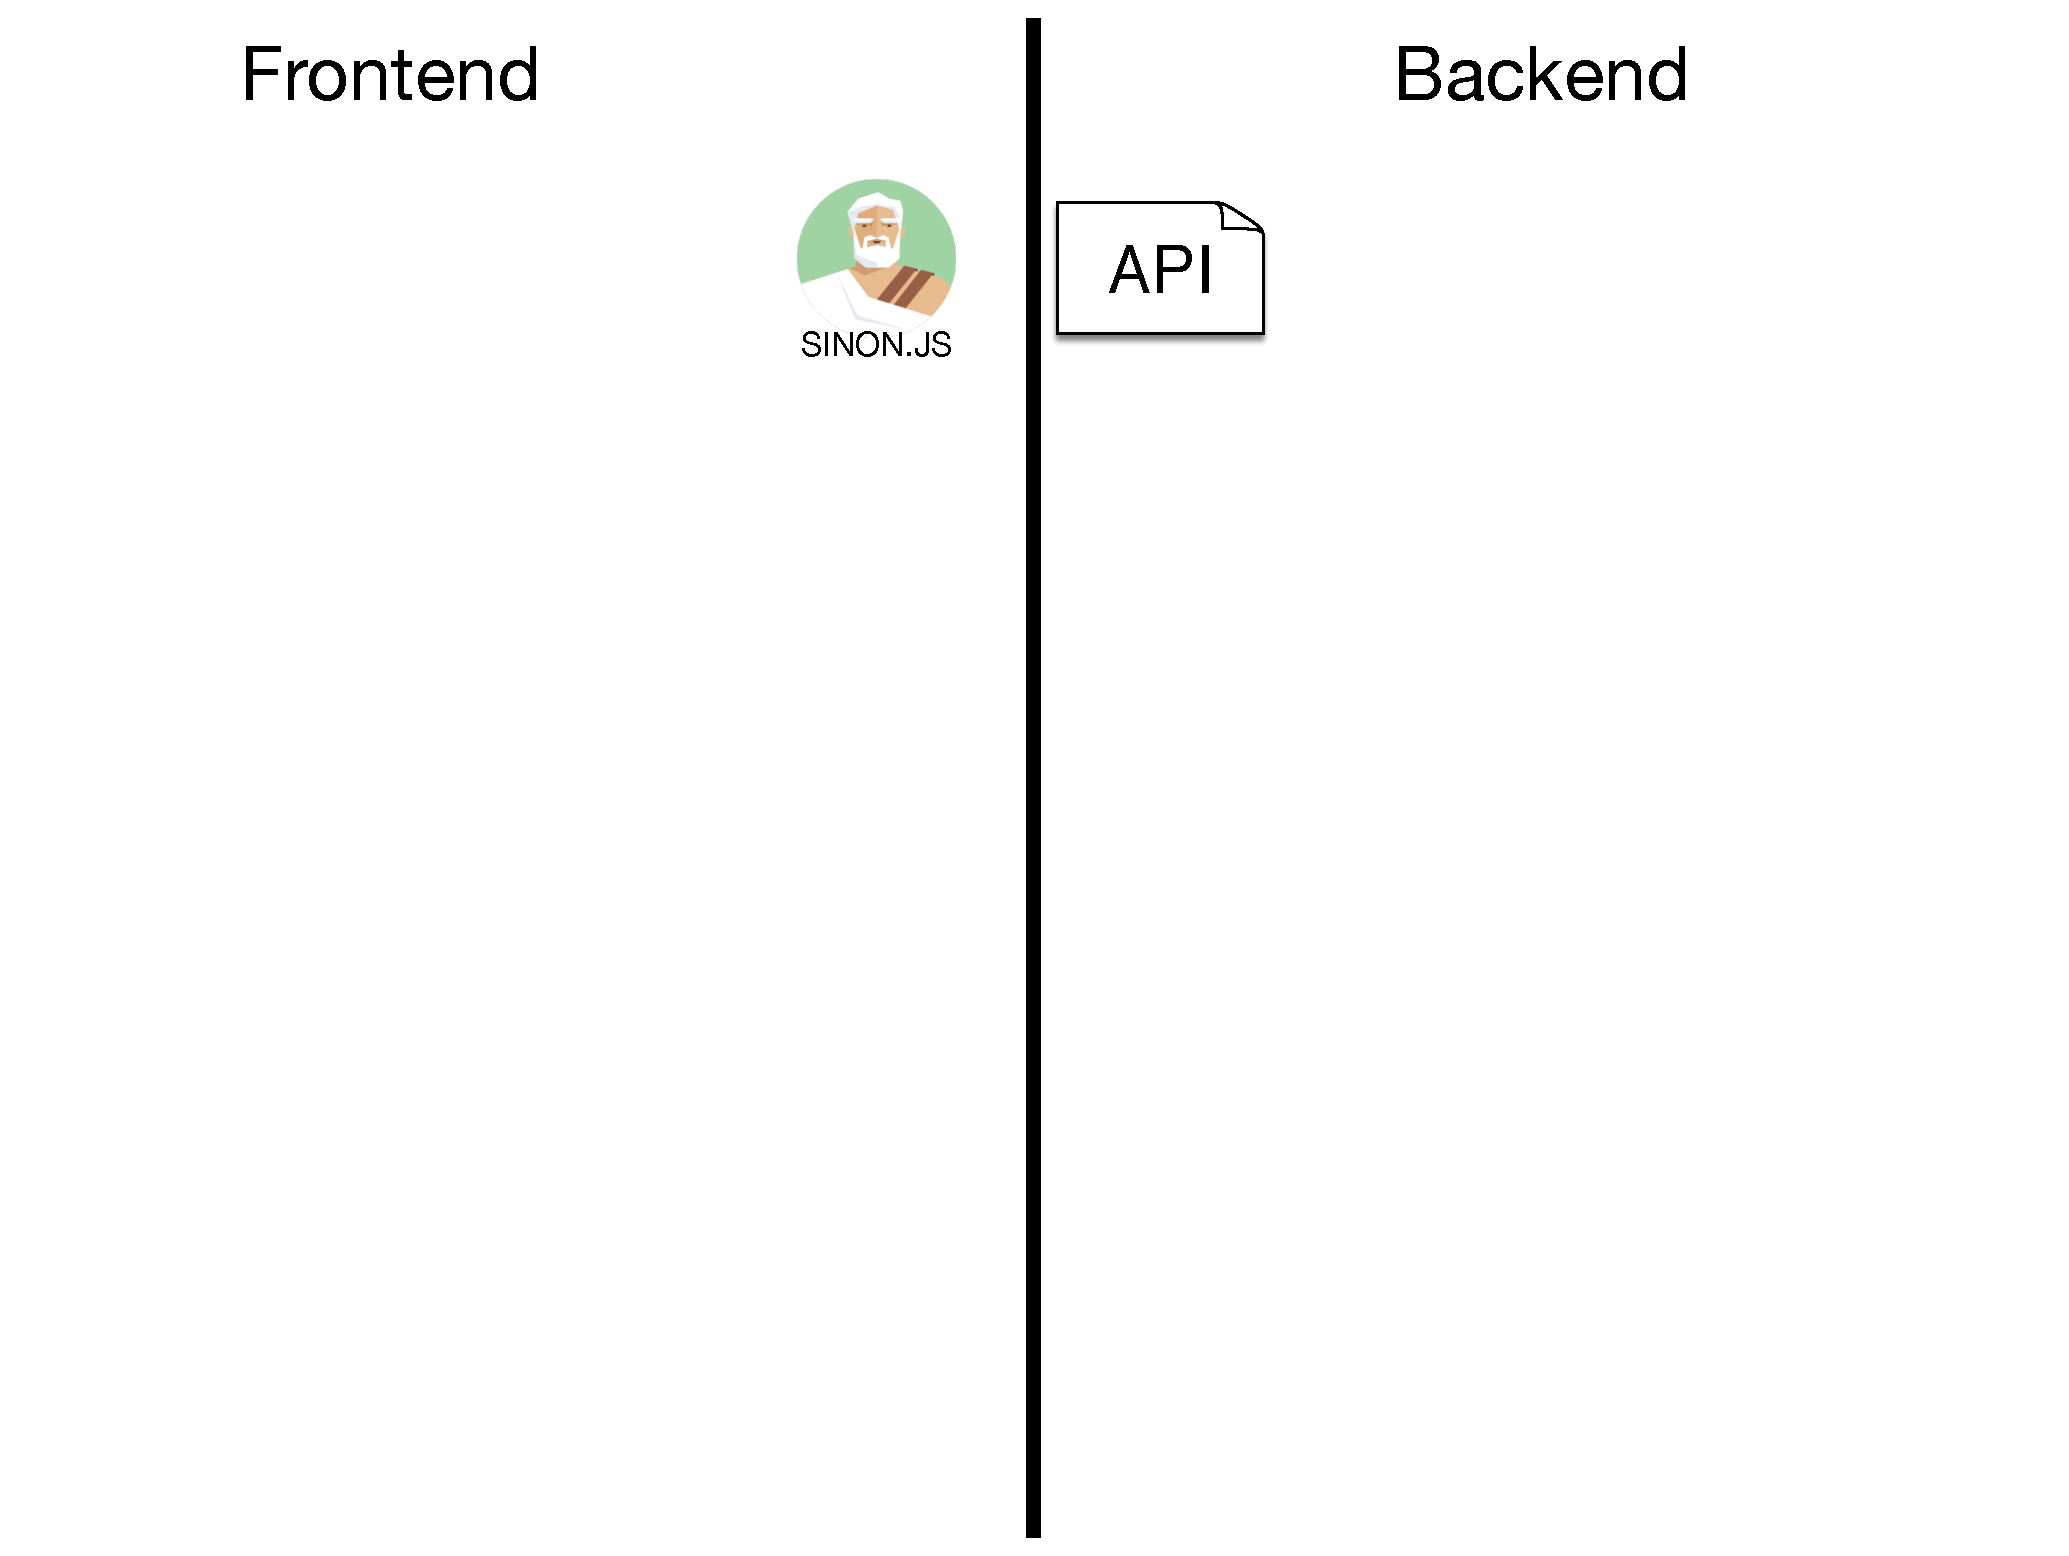
\includegraphics[width=\textwidth]{images/still-quite-naive-approach-2.pdf}
}

\only<4>{
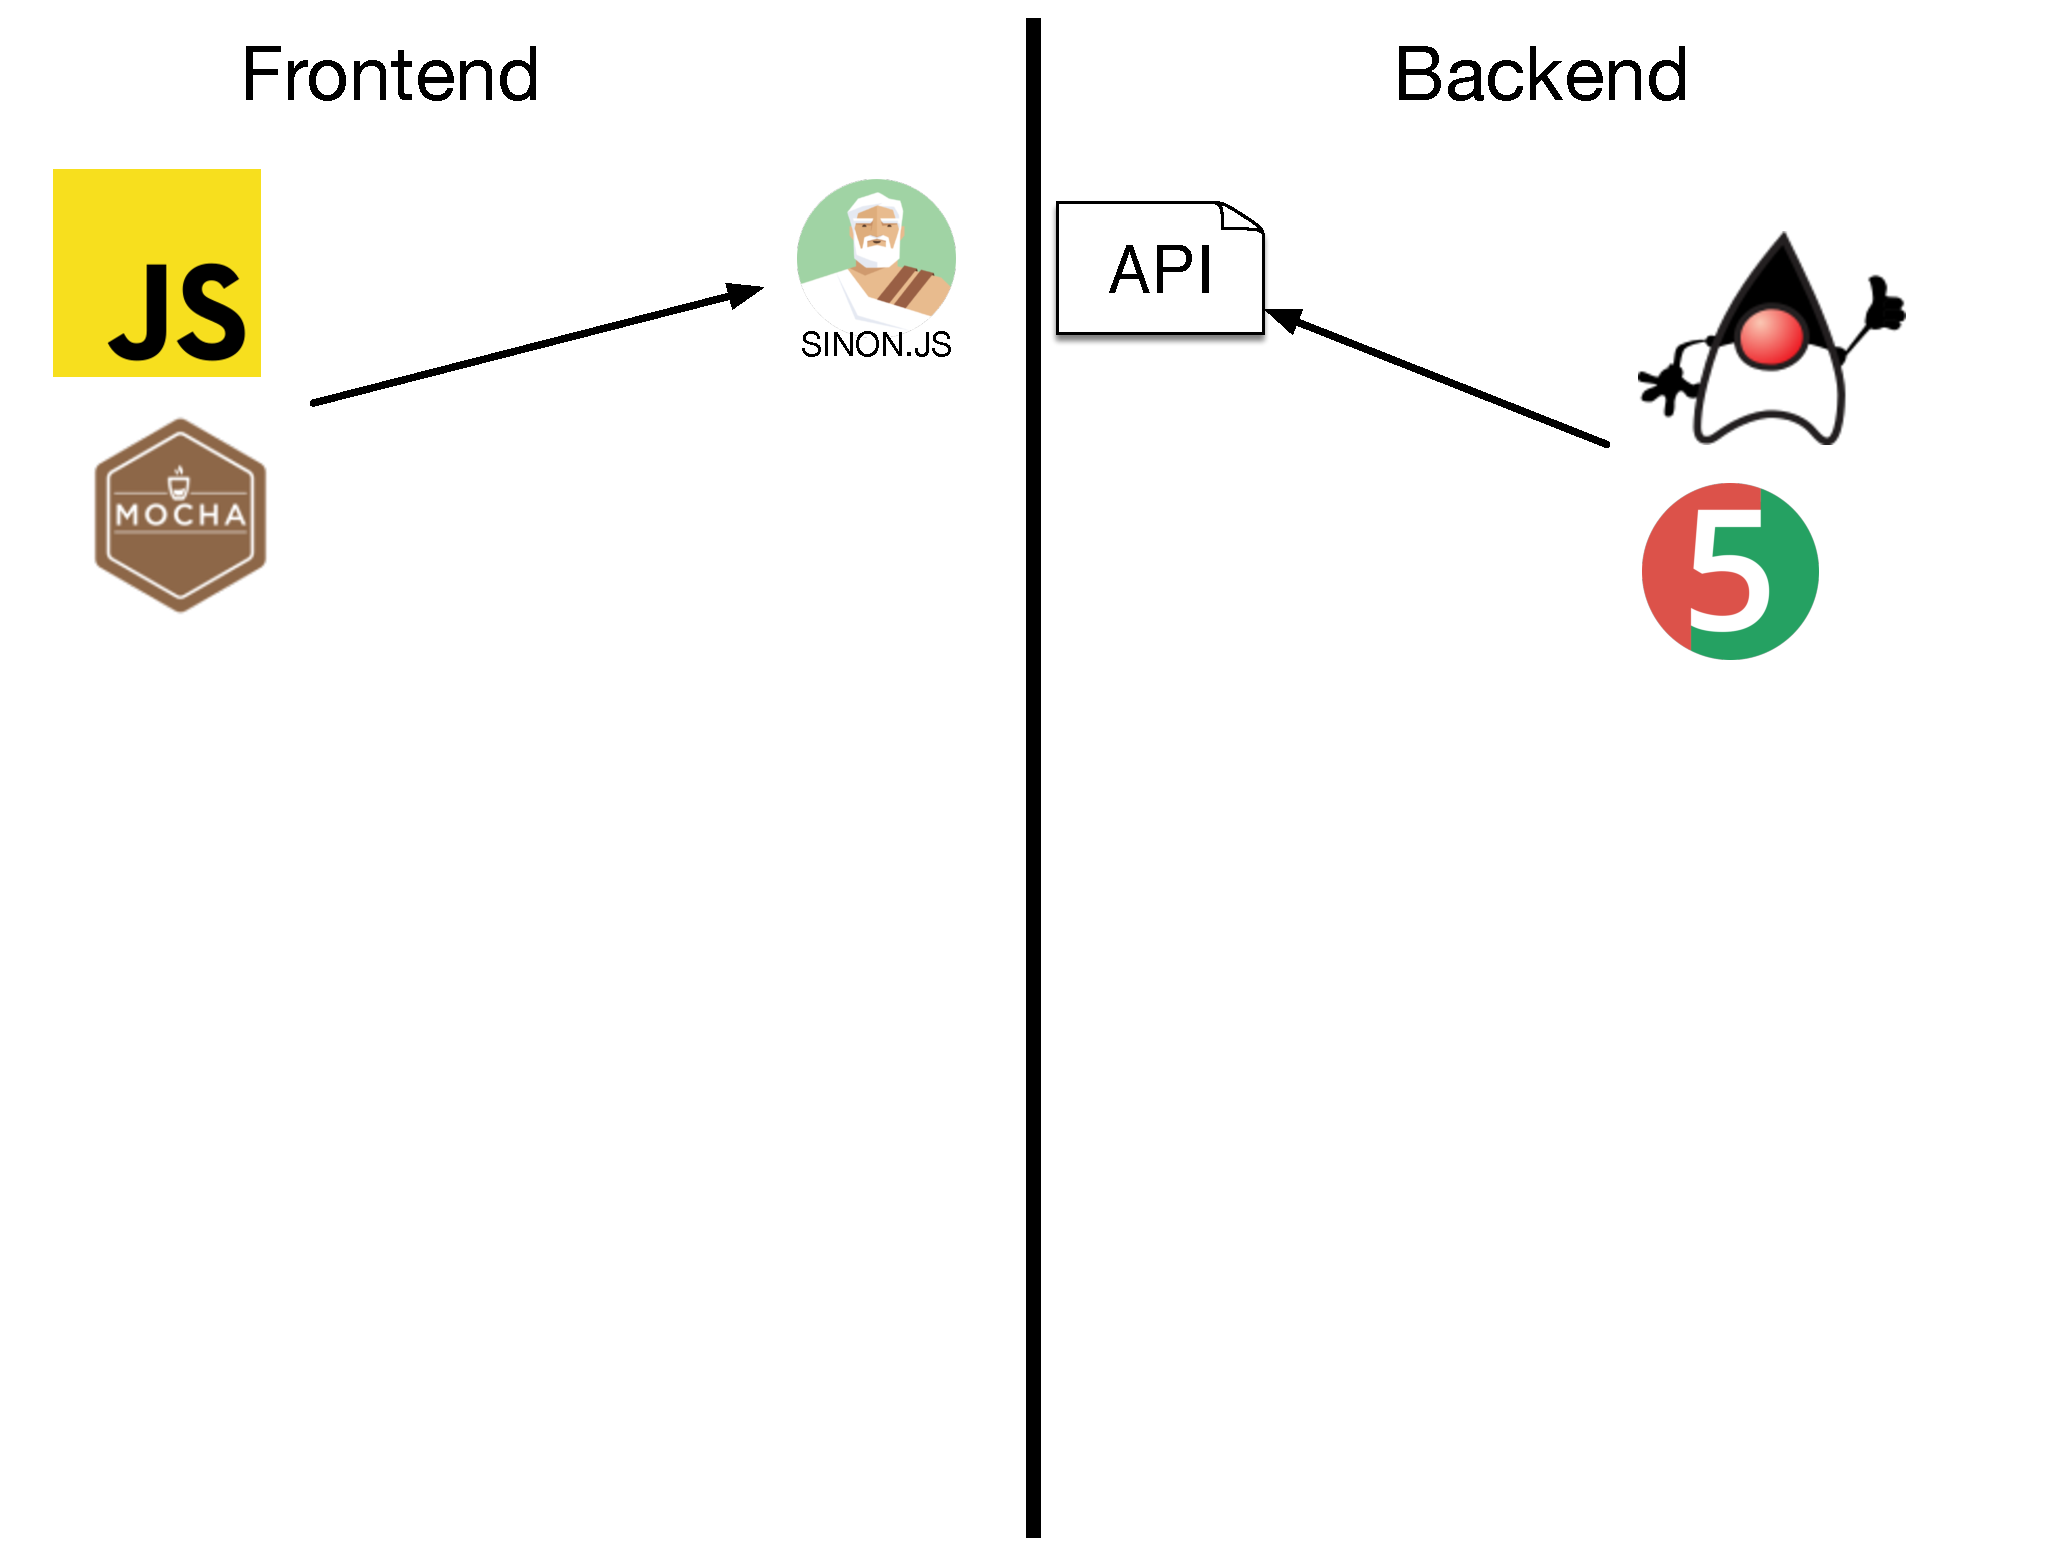
\includegraphics[width=\textwidth]{images/still-quite-naive-approach-3.pdf}
}

\only<5>{
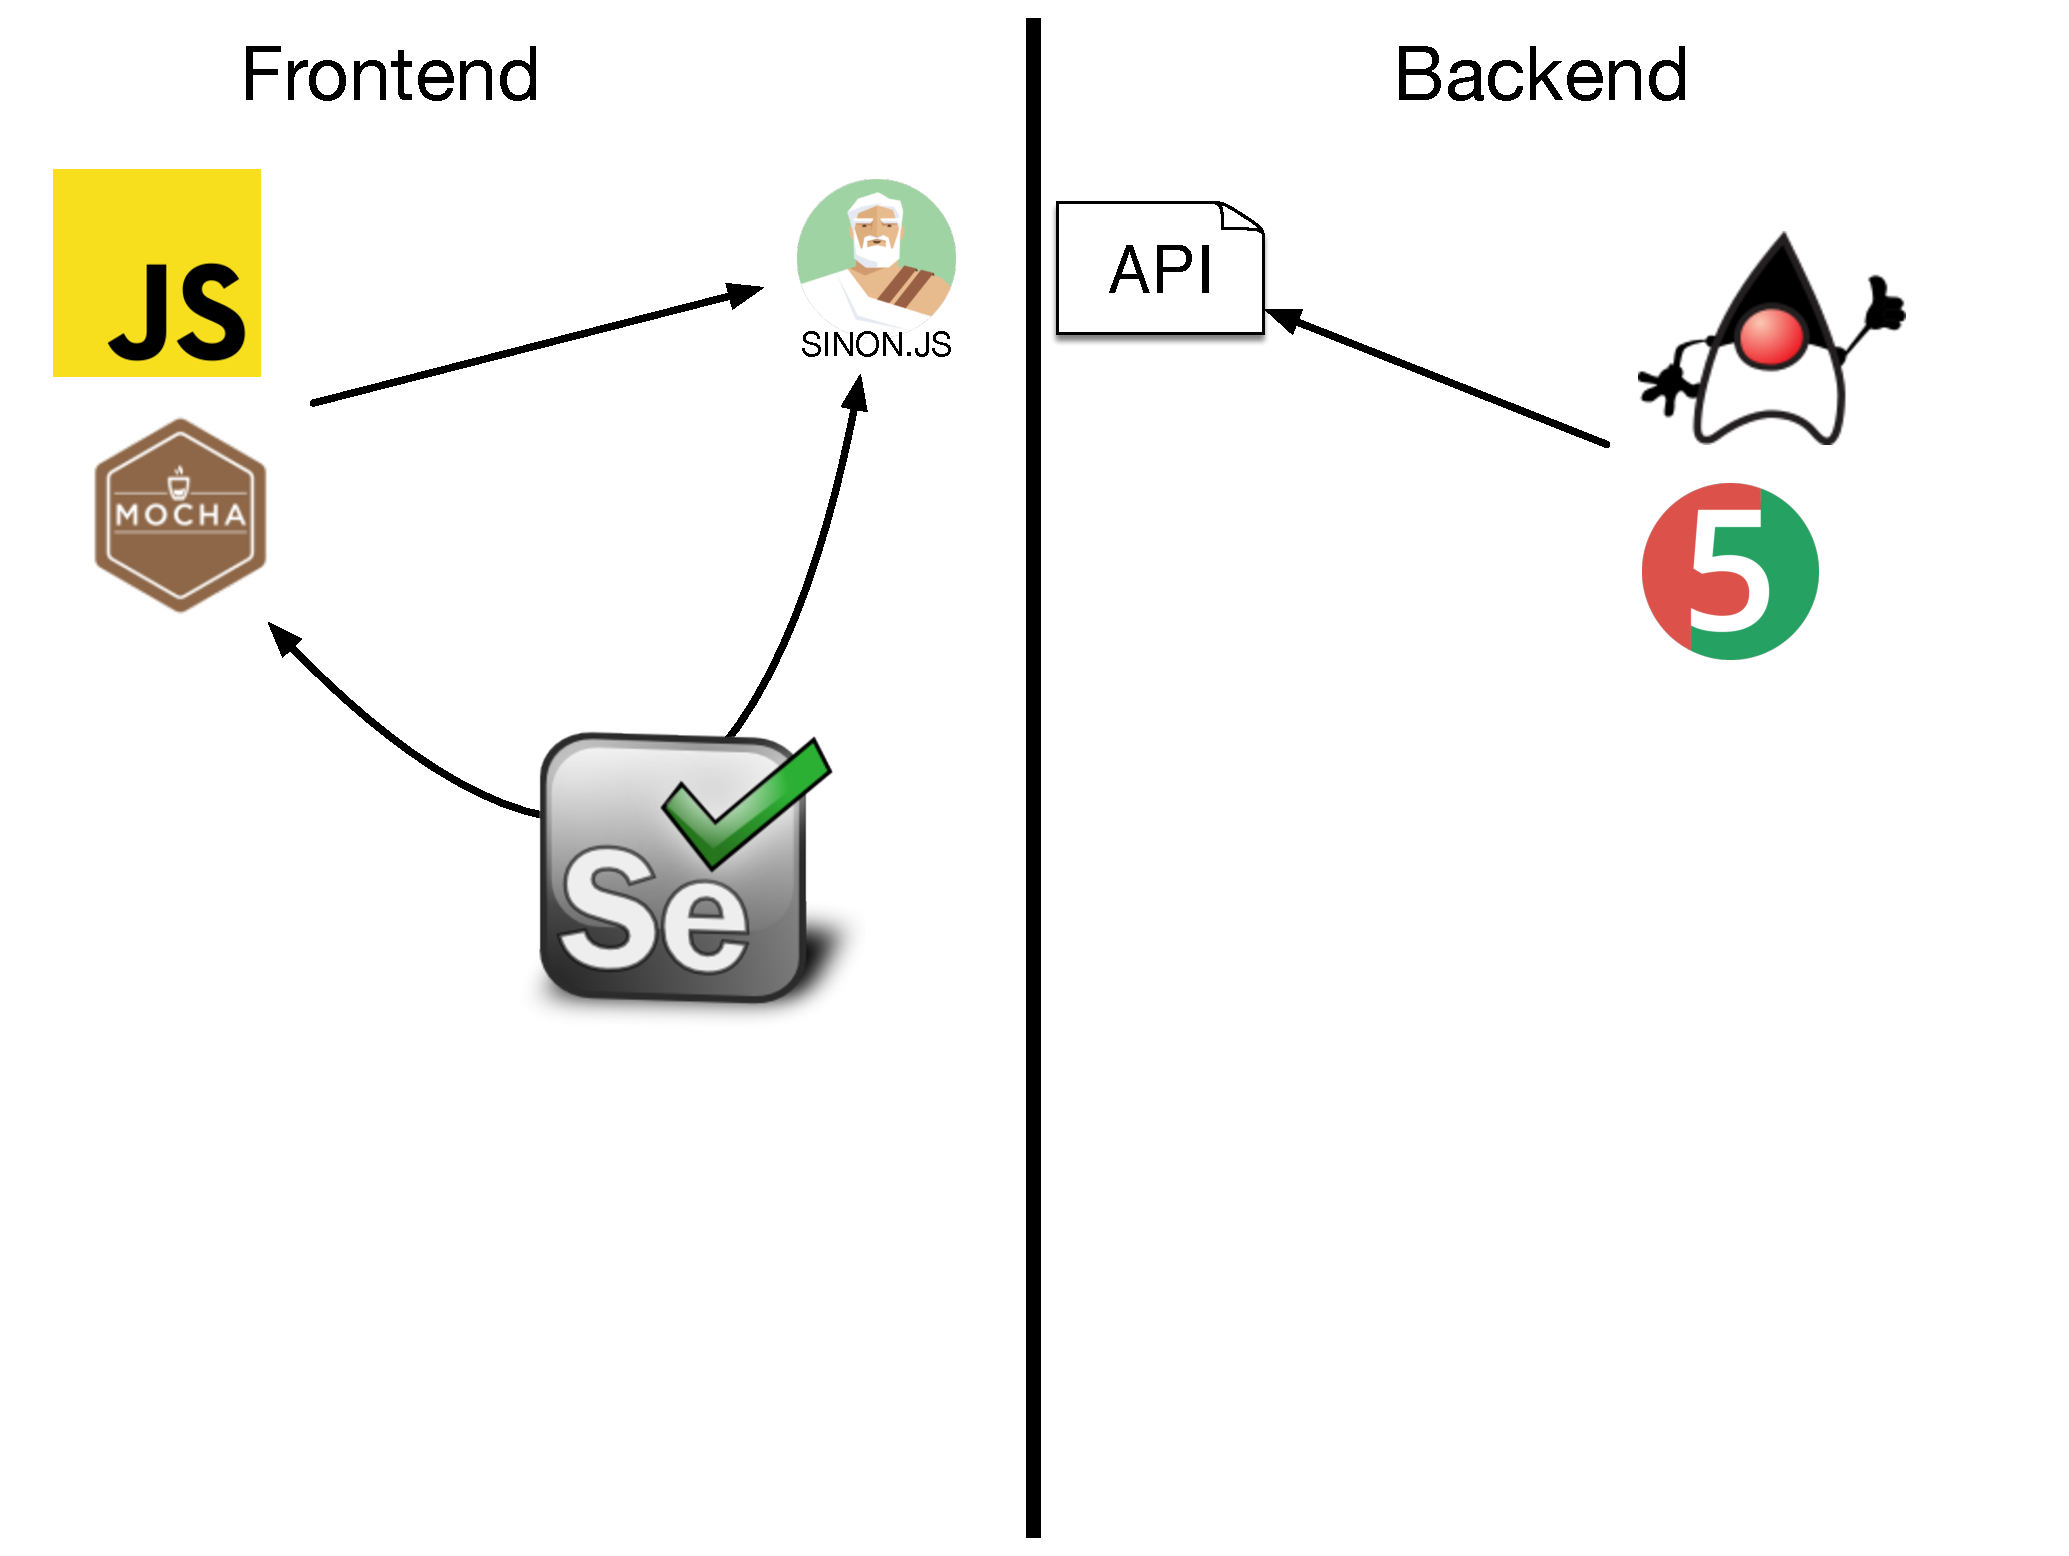
\includegraphics[width=\textwidth]{images/still-quite-naive-approach-4.pdf}
}

\end{frame}

\begin{frame}[fragile]{}

\begin{center}
{\Huge
But $\ldots$
}
\end{center}

\end{frame}

\begin{frame}[fragile]{}

\only<1>{
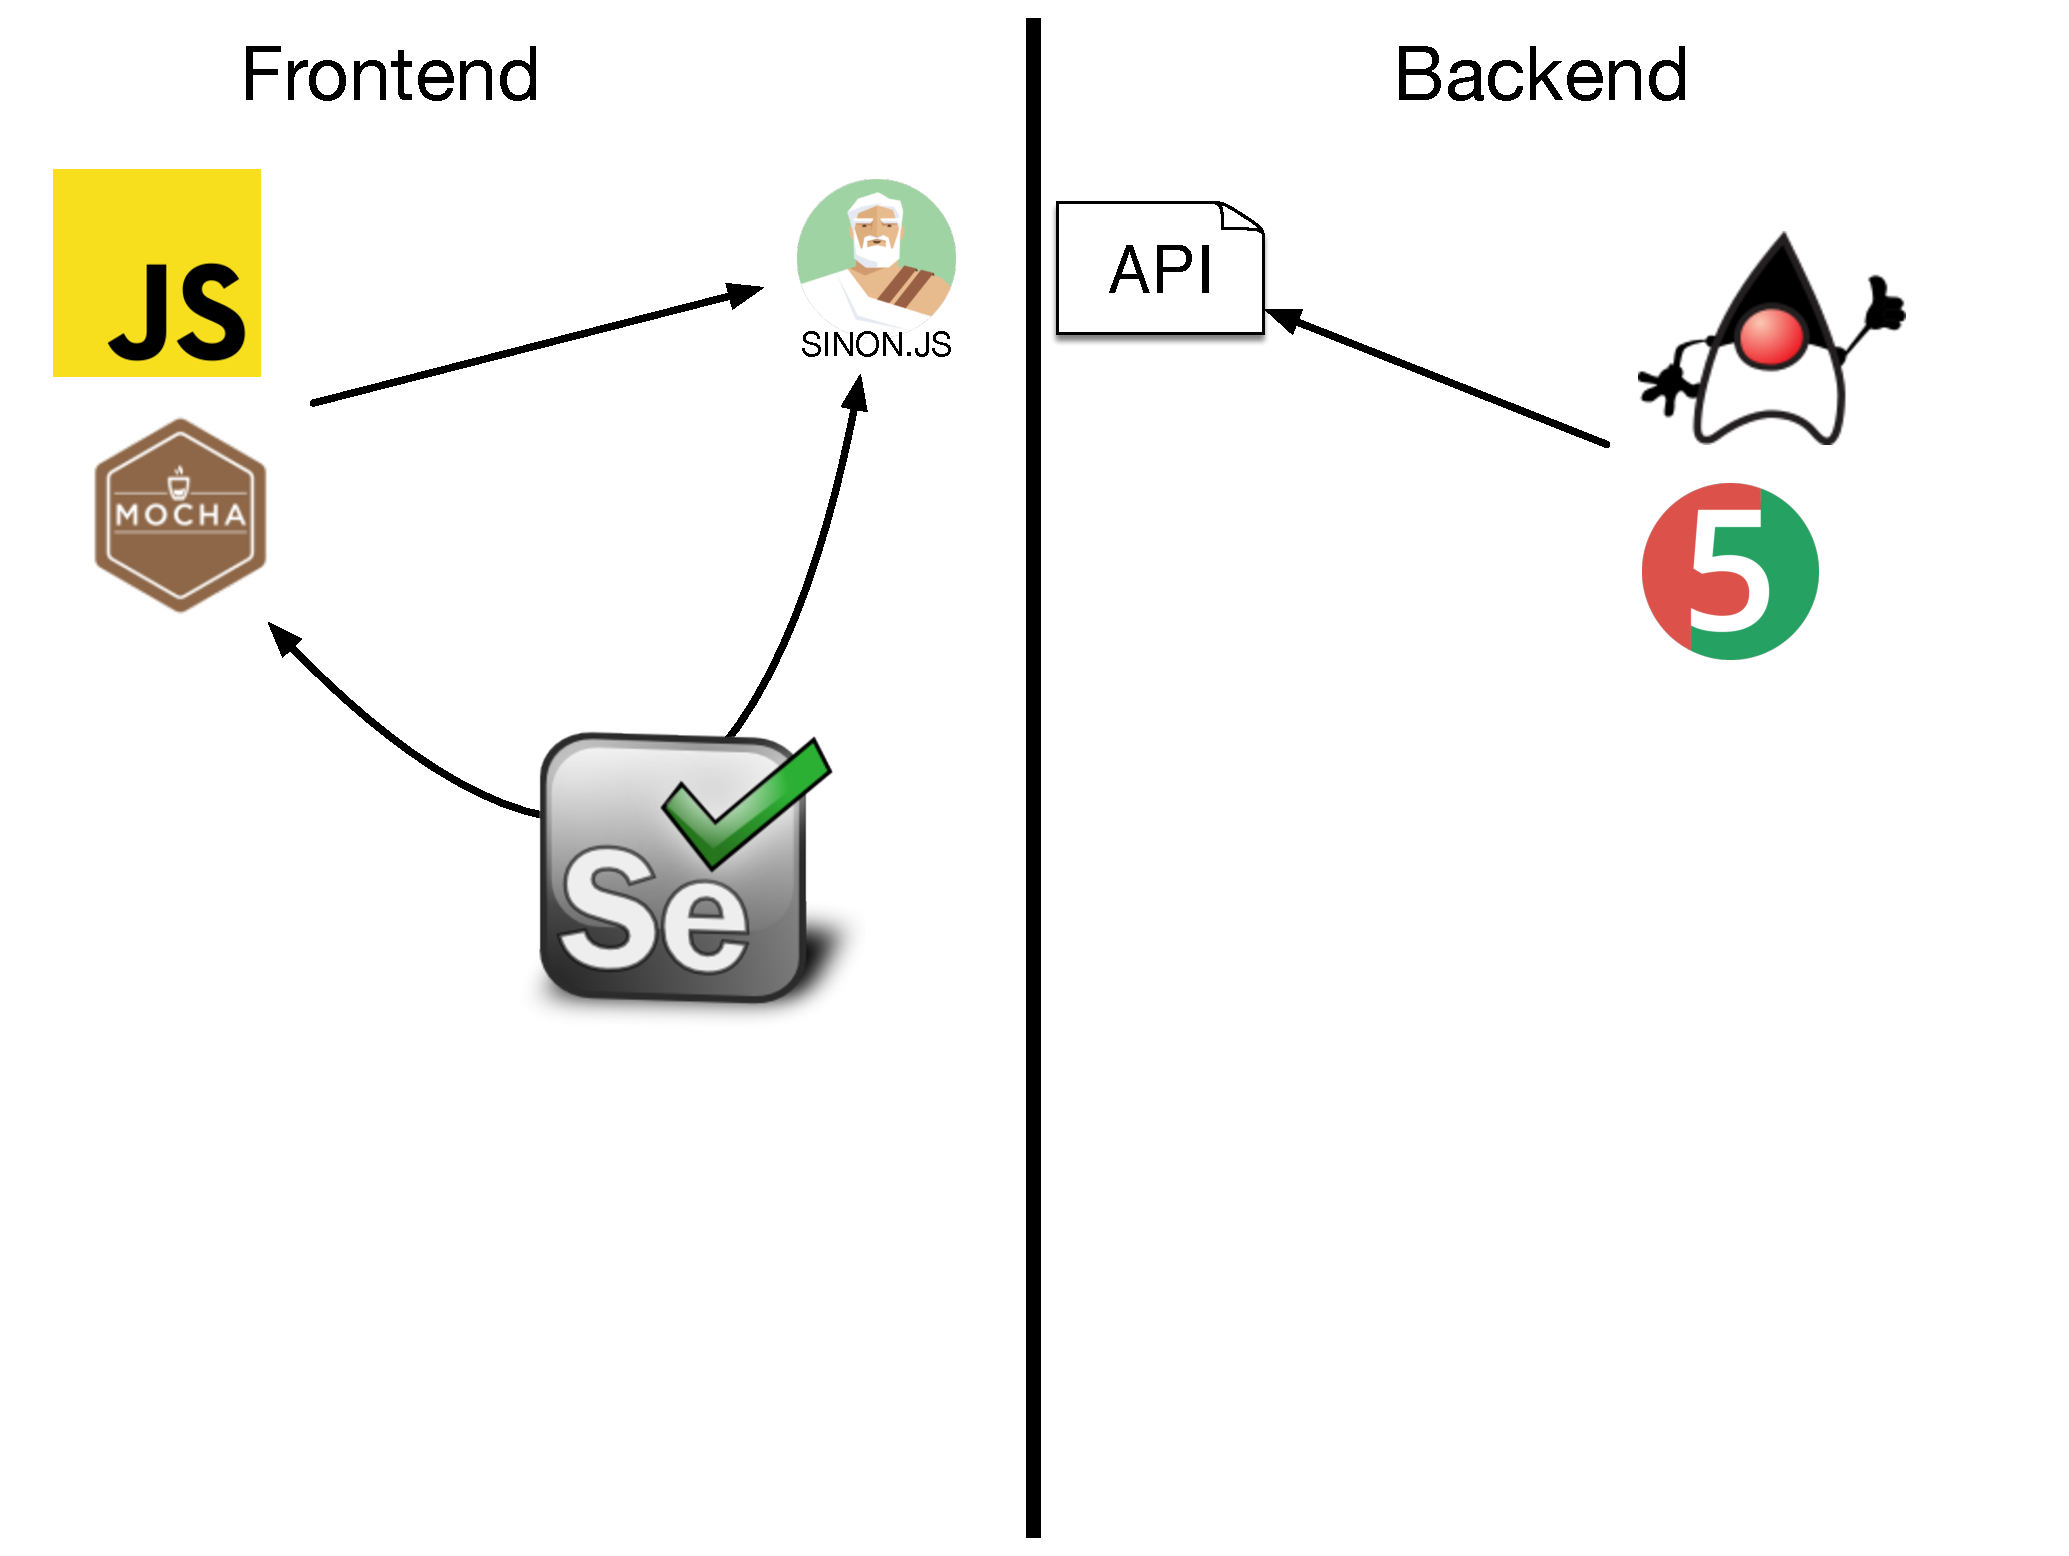
\includegraphics[width=\textwidth]{images/still-quite-naive-approach-4.pdf}
}

\only<2>{
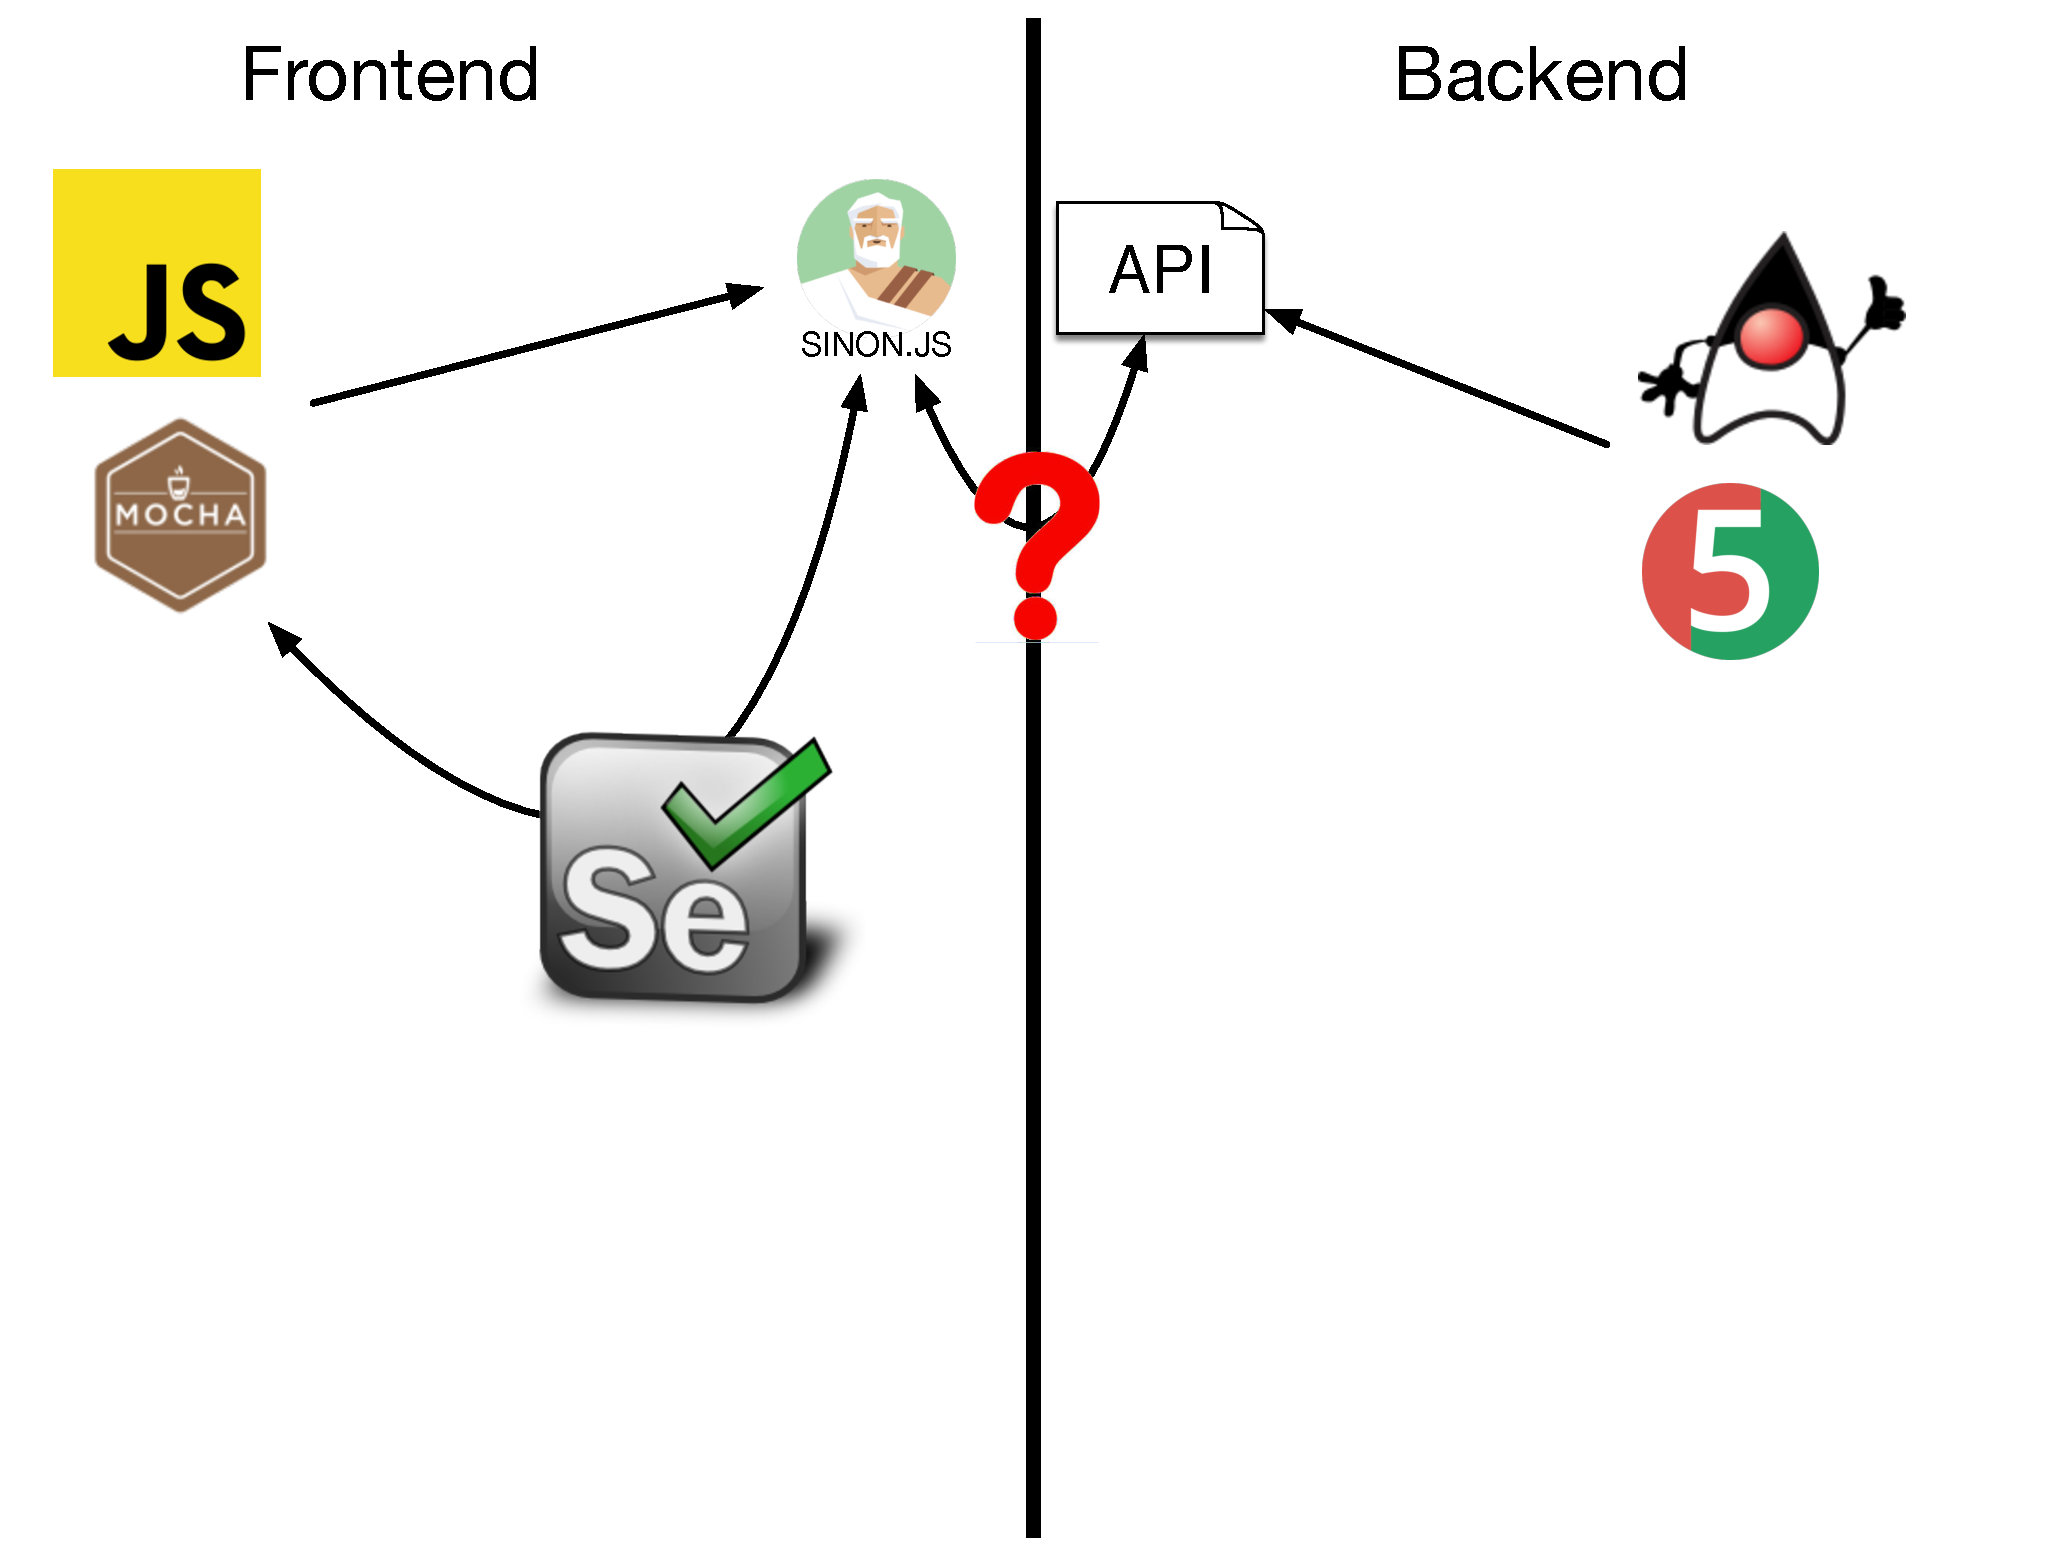
\includegraphics[width=\textwidth]{images/still-quite-naive-approach-5.pdf}
}

\only<3>{
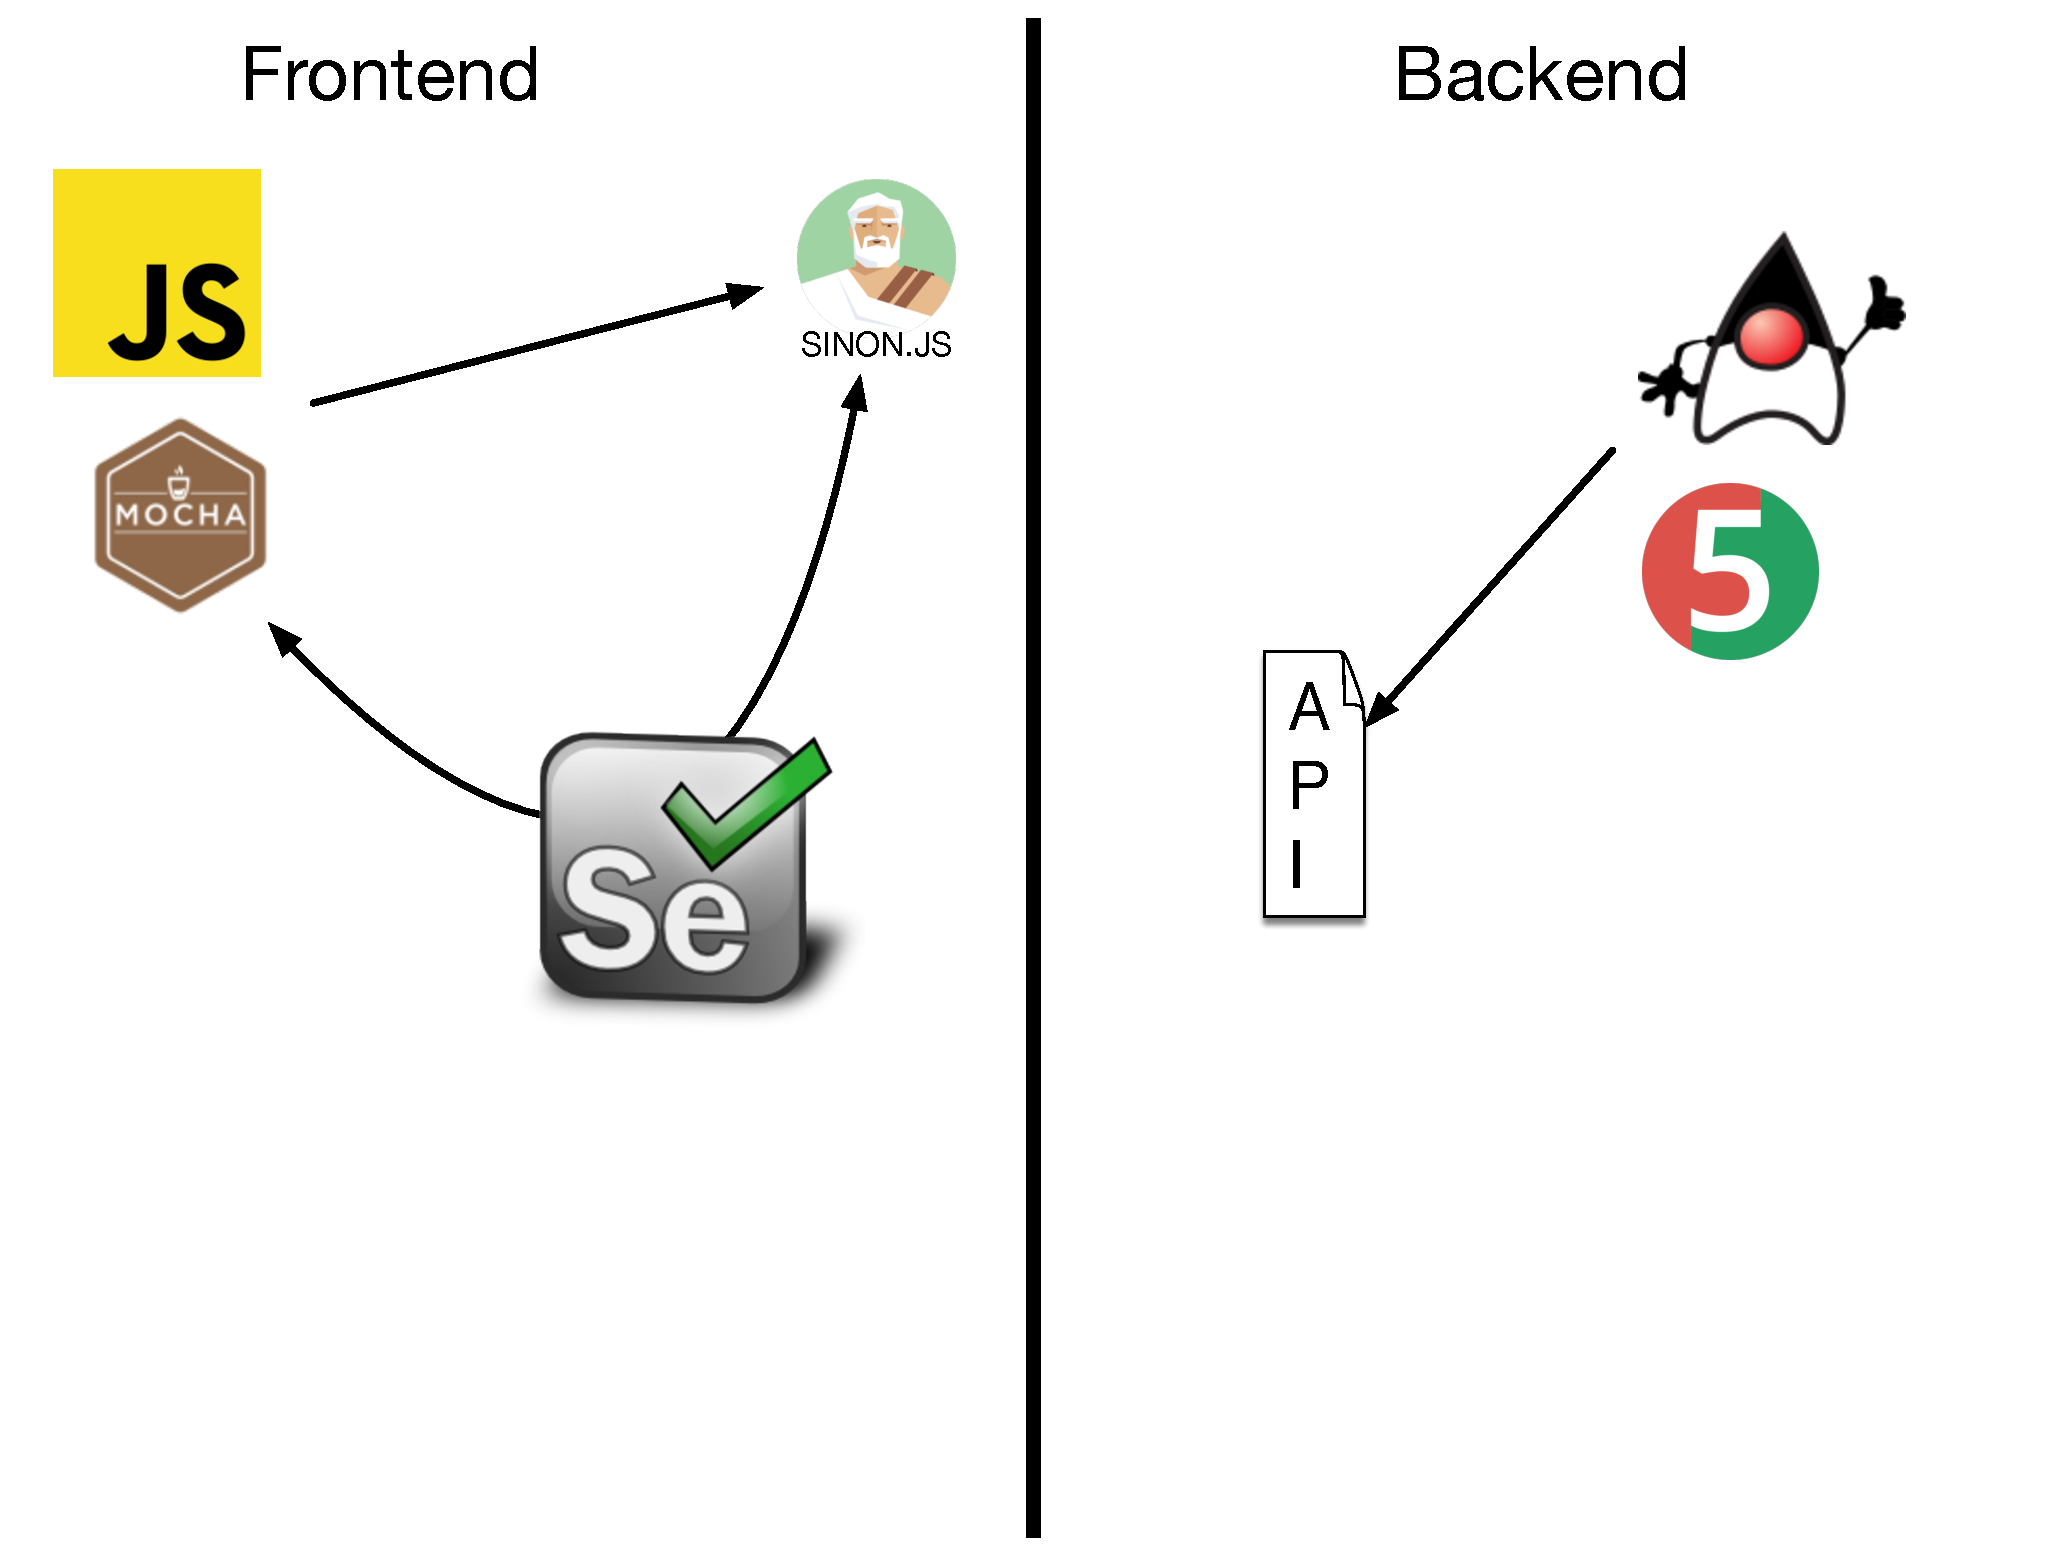
\includegraphics[width=\textwidth]{images/still-quite-naive-approach-6.pdf}
}

\only<4>{
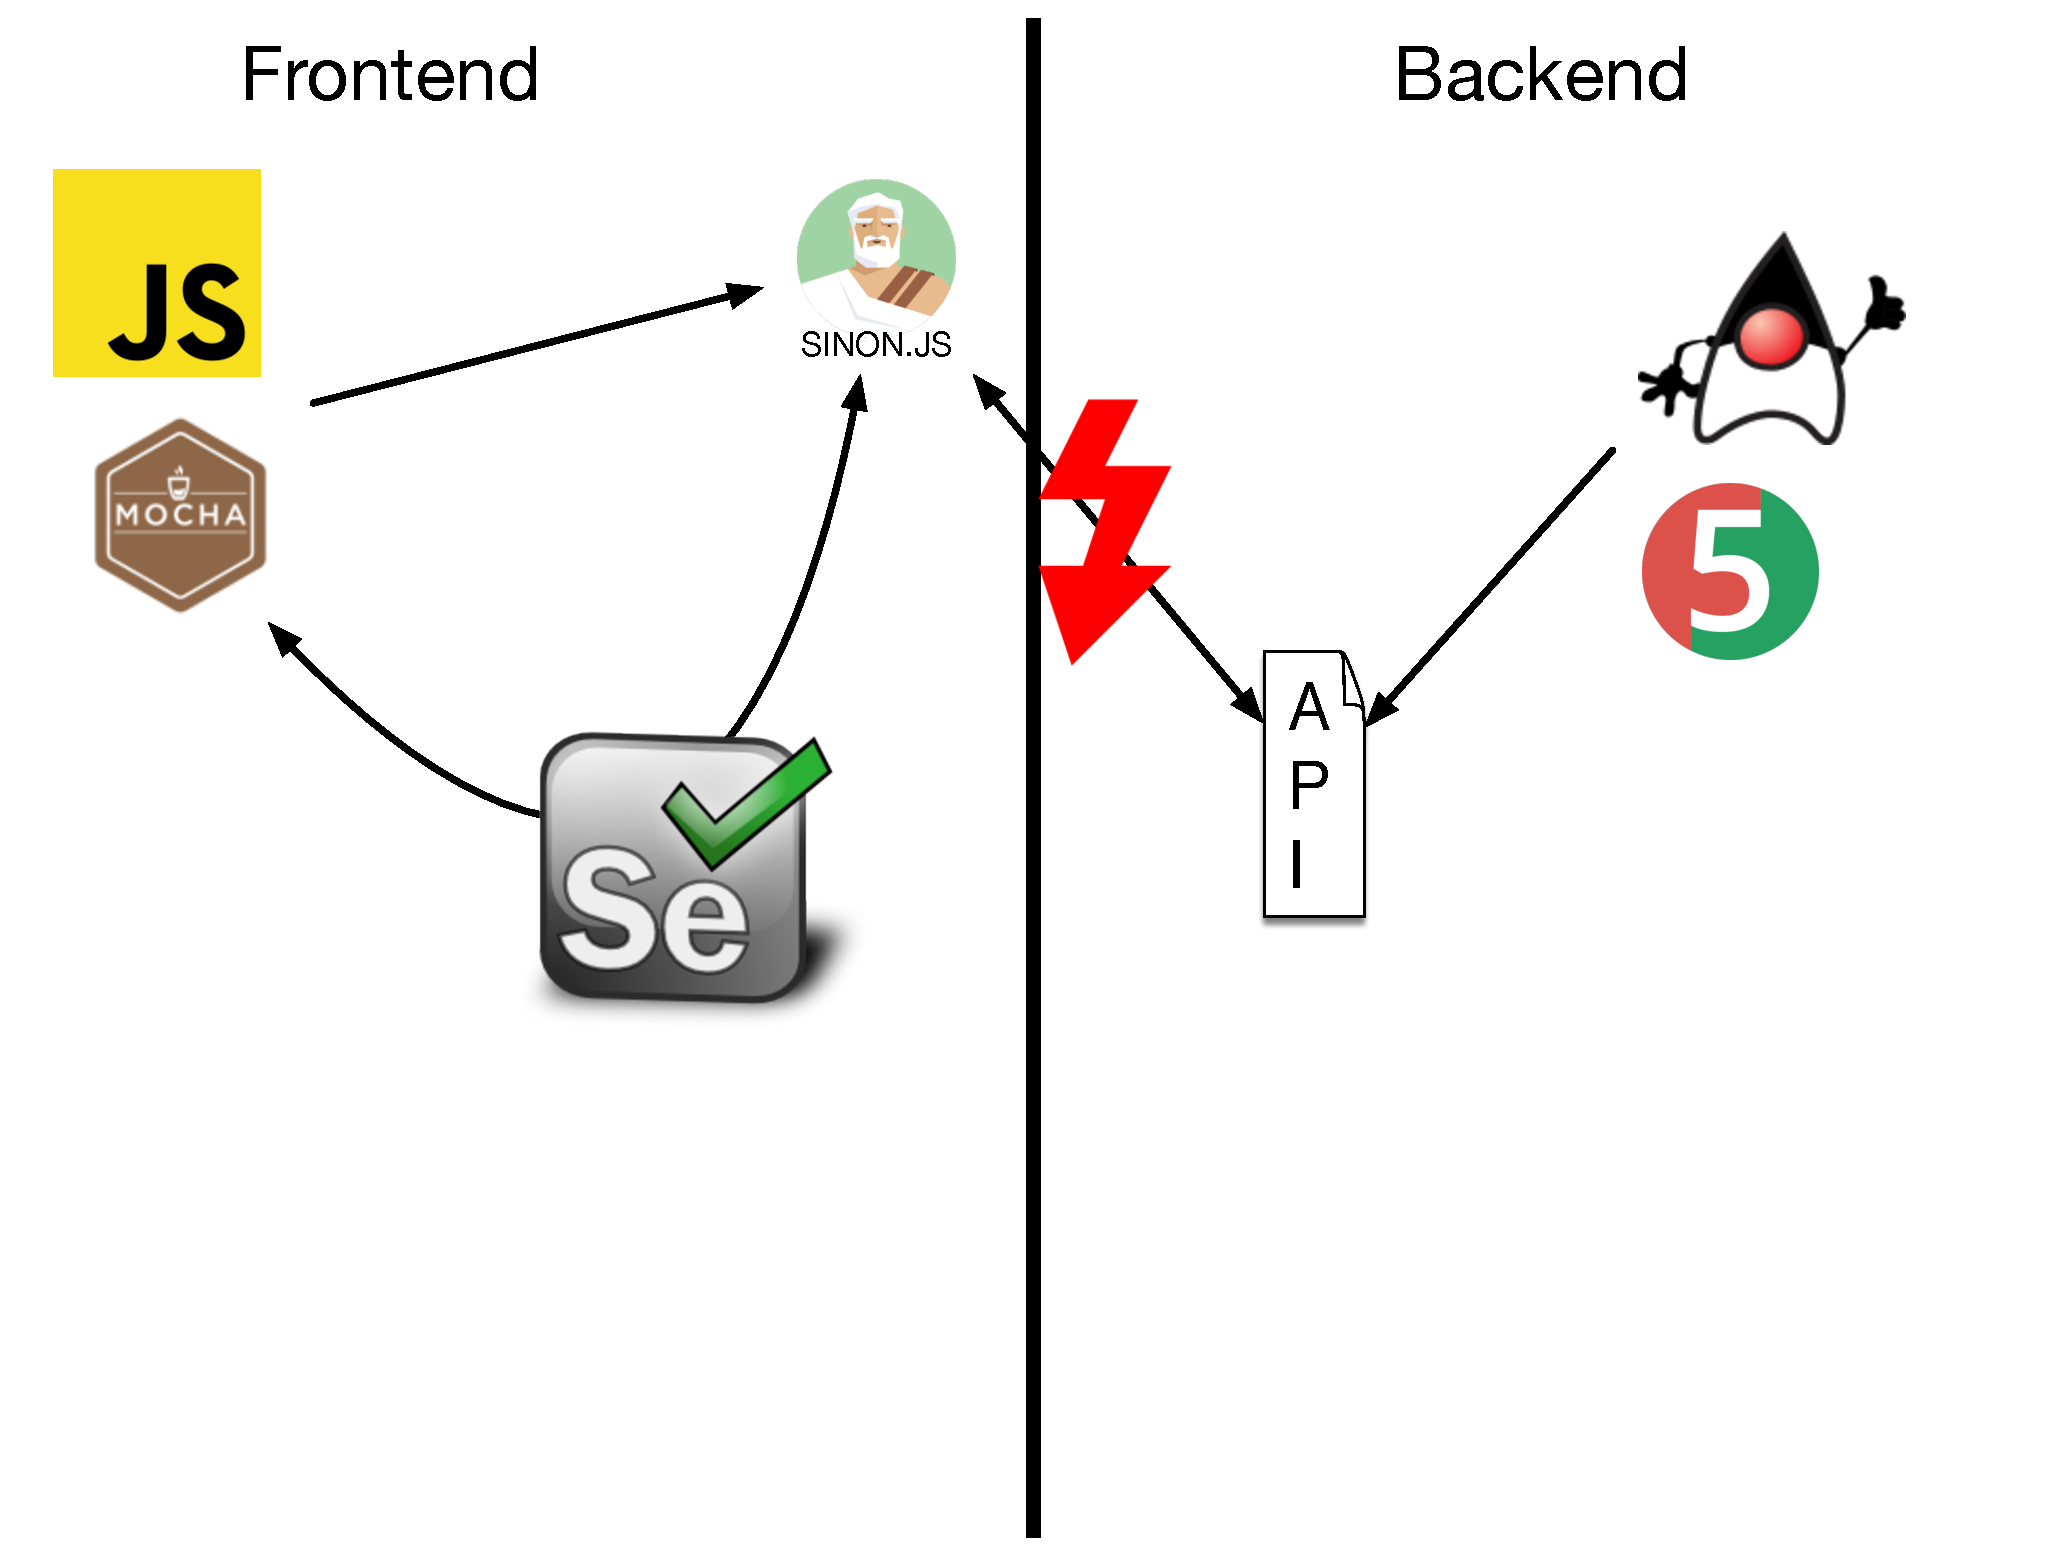
\includegraphics[width=\textwidth]{images/still-quite-naive-approach-7.pdf}
}

\end{frame}

%%%%%%%%%%%%%%%%%%%%%%%%%%%%%%%%%%%%%%%%%%%%%%%%%%
\begin{frame}[fragile]{}

\begin{center}
{\Huge
``Industry-Strength'' Approach: \\[1em]
Consumer-Driven Contract Testing
}
\end{center}

\end{frame}

\begin{frame}[fragile]{}

\only<1>{
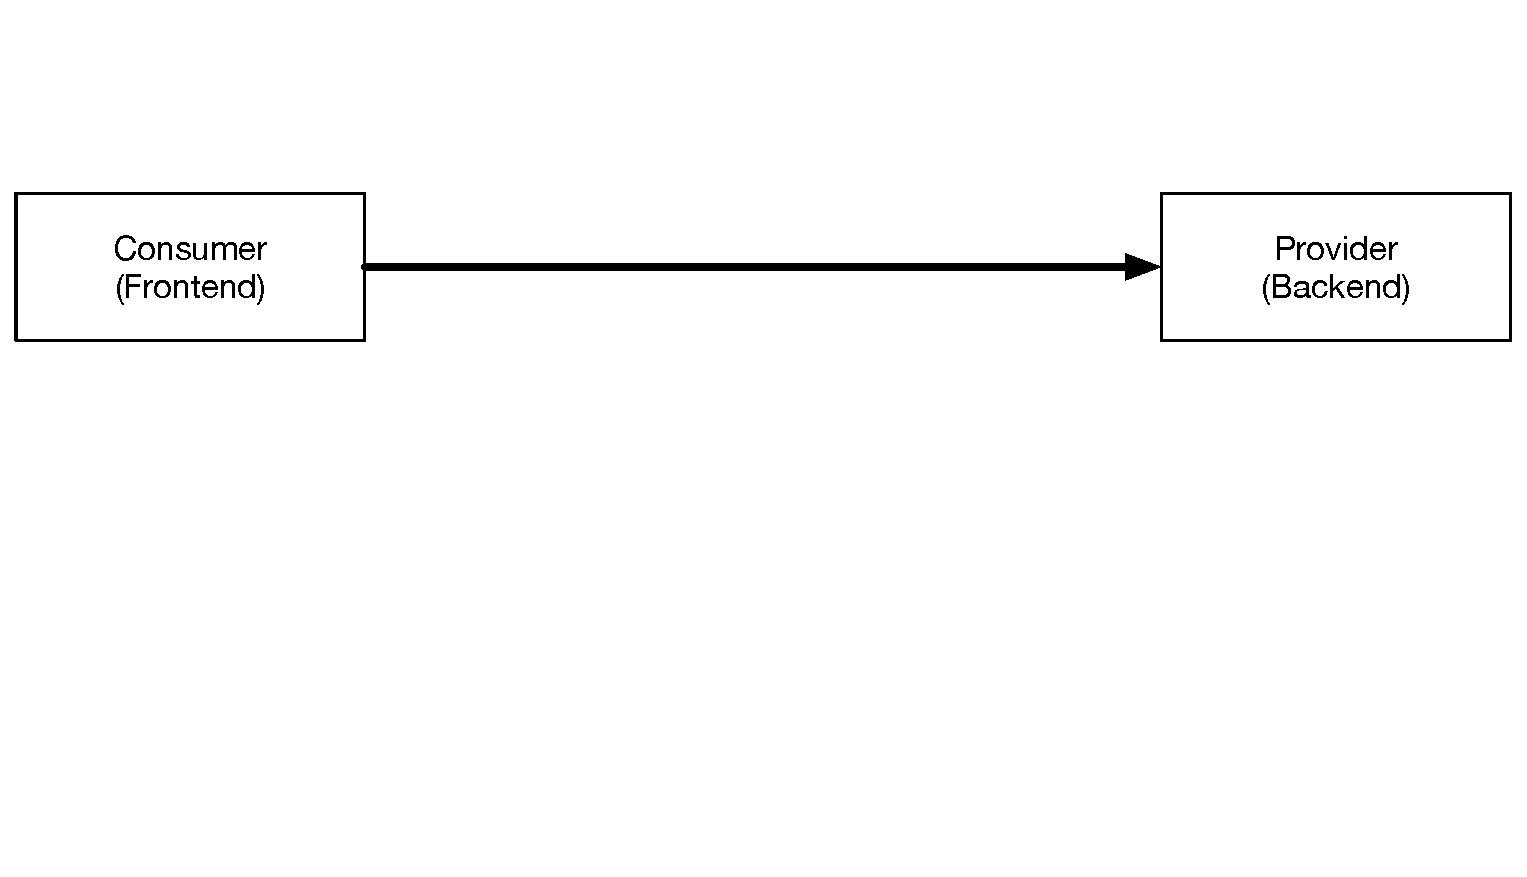
\includegraphics[width=\textwidth]{images/CDCT1.pdf}
}

\only<2>{
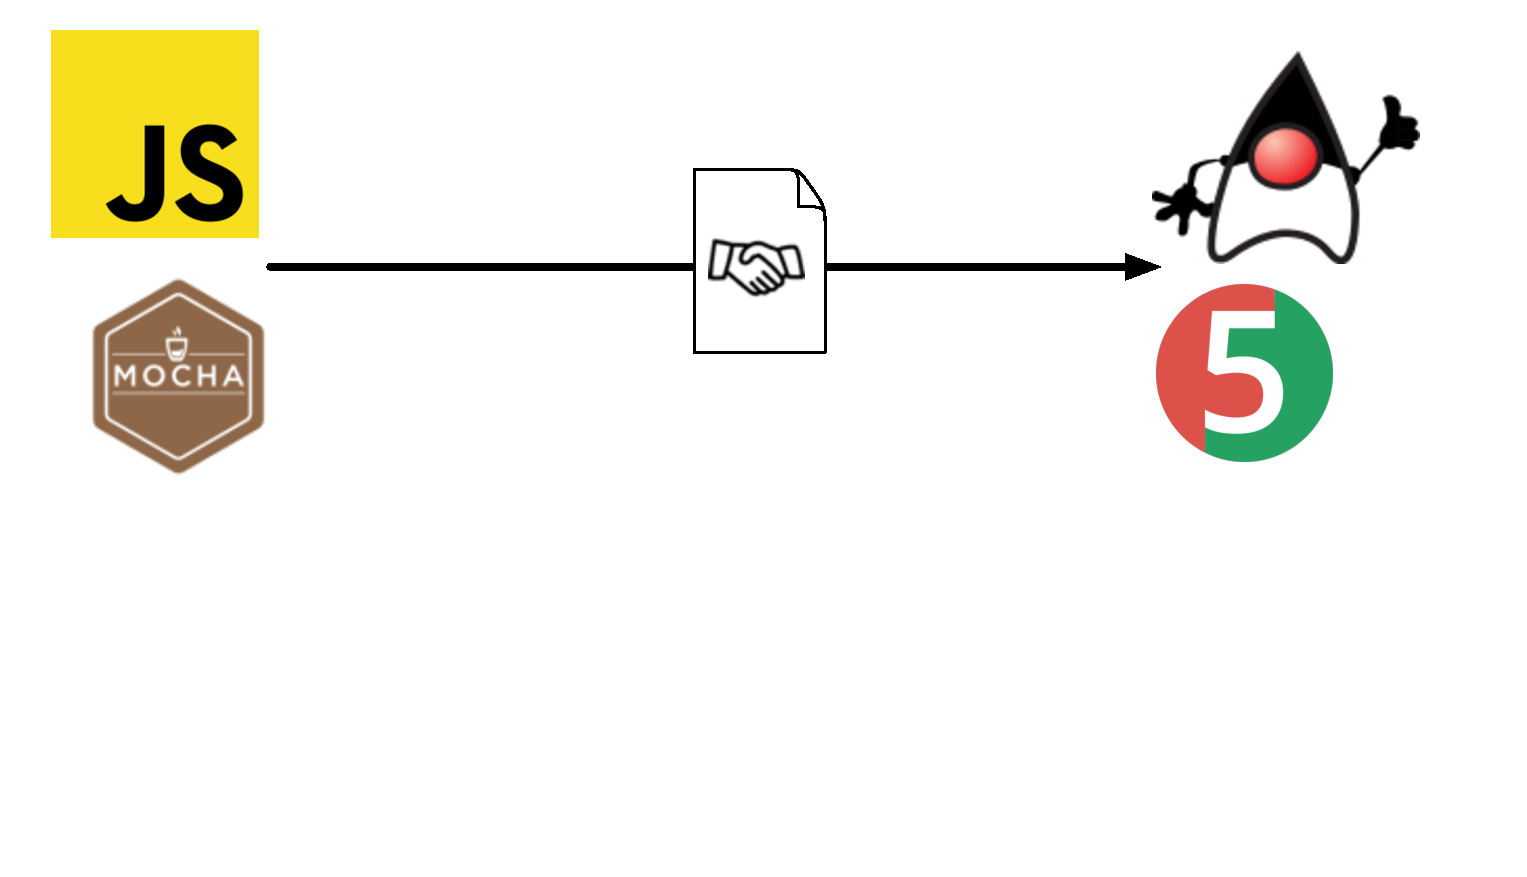
\includegraphics[width=\textwidth]{images/CDCT2.pdf}
}

\only<3>{
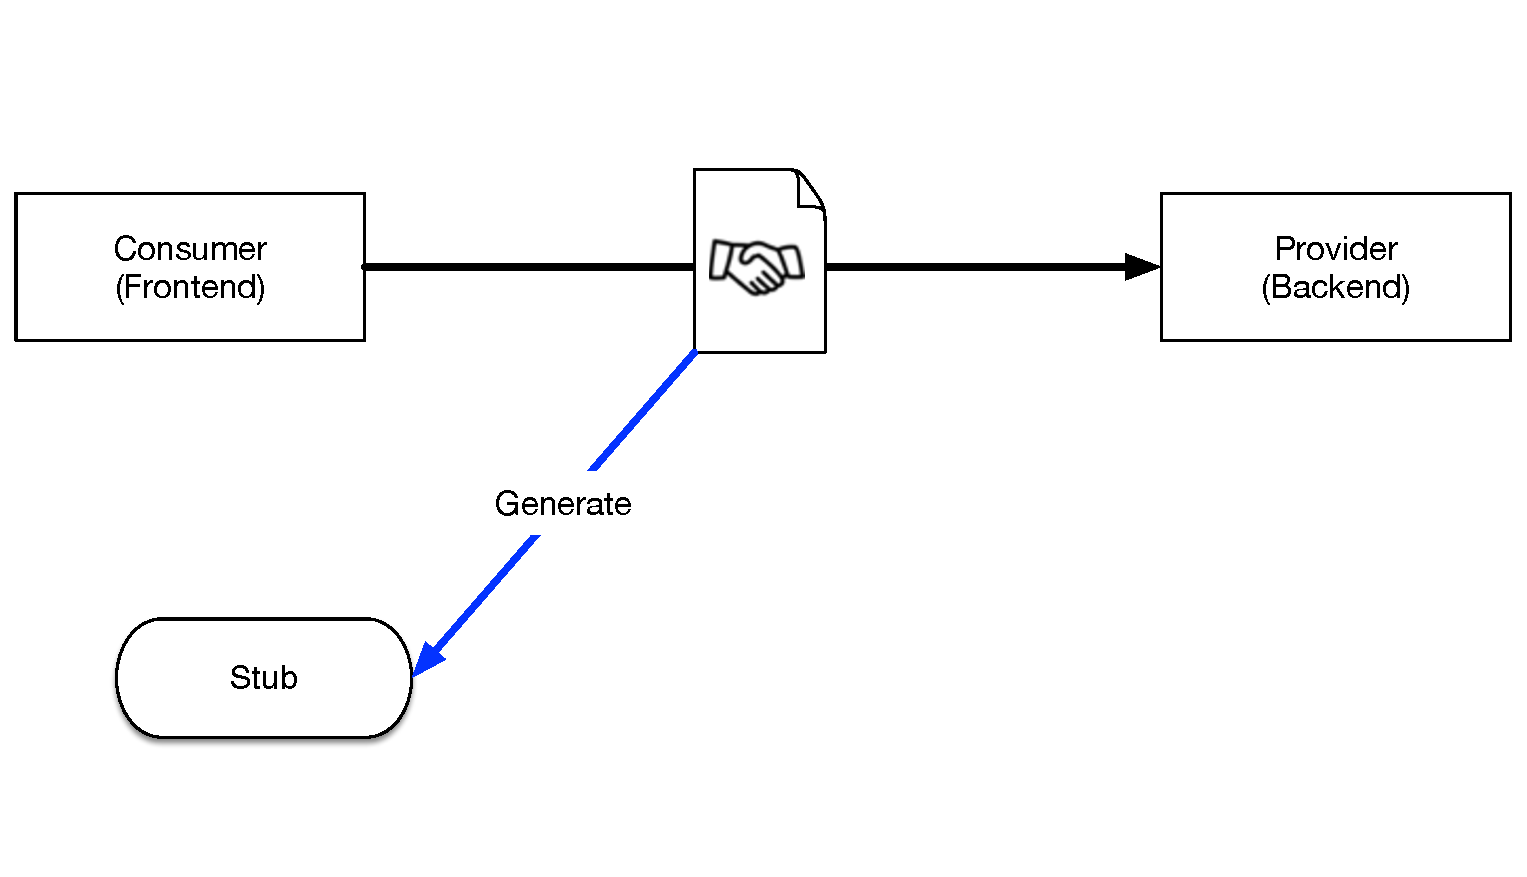
\includegraphics[width=\textwidth]{images/CDCT3.pdf}
}

\only<4>{
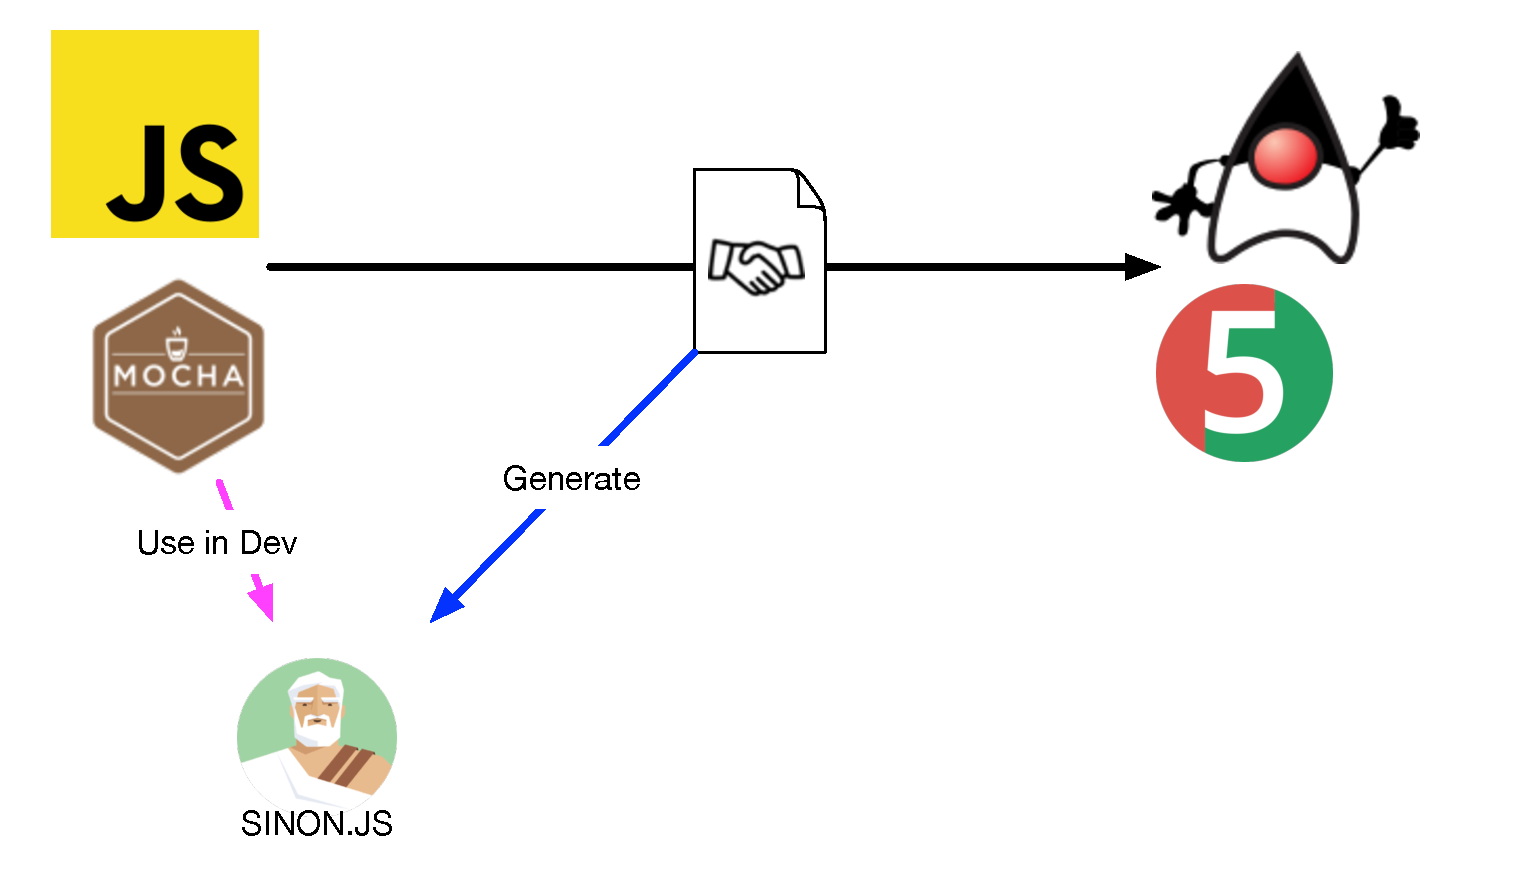
\includegraphics[width=\textwidth]{images/CDCT4.pdf}
}

\only<5>{
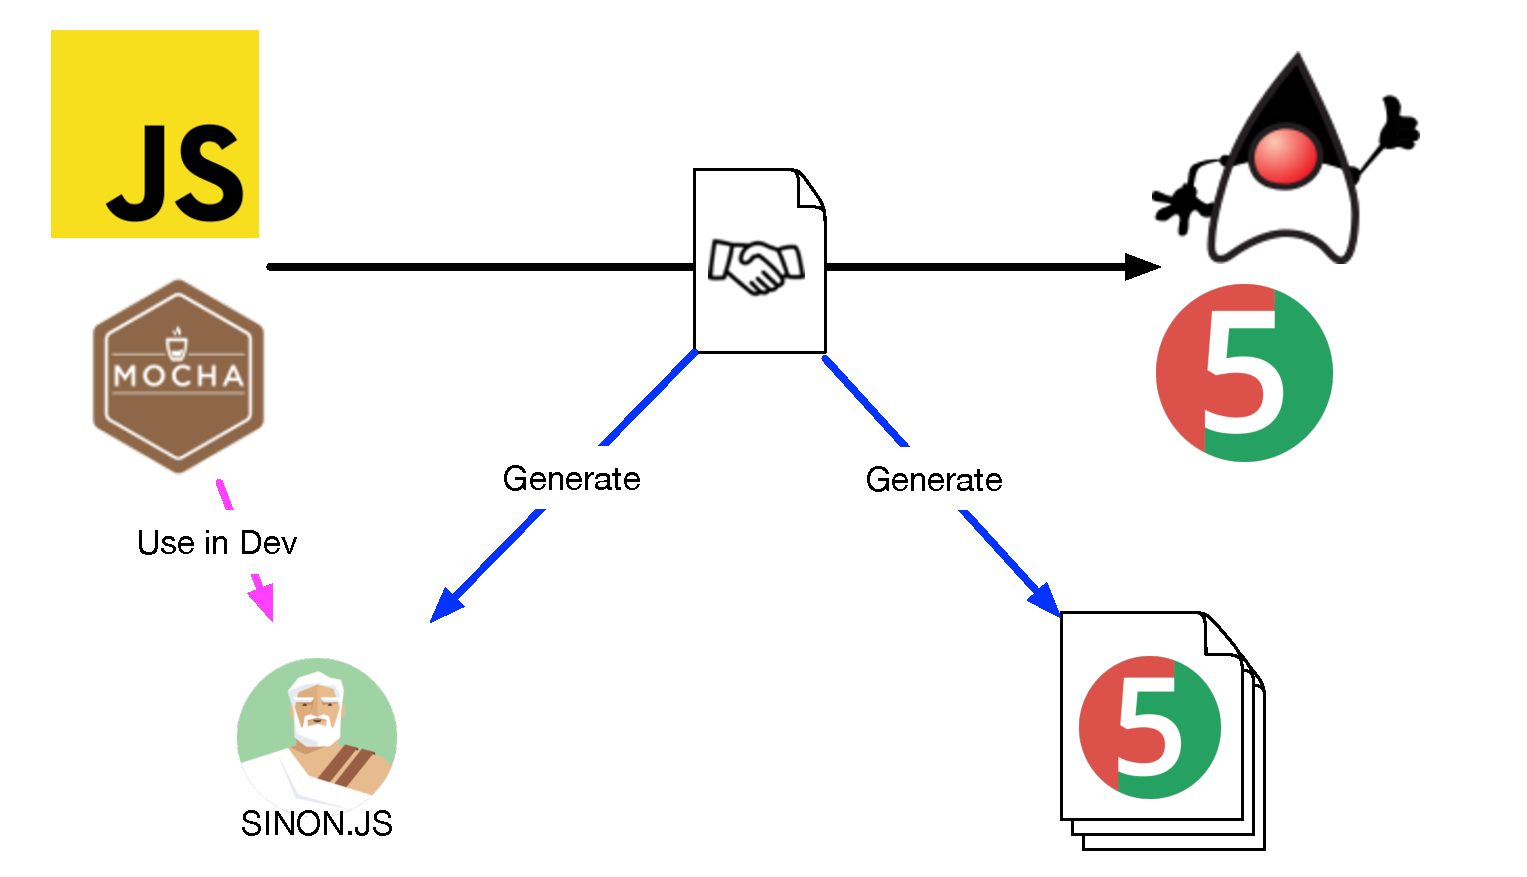
\includegraphics[width=\textwidth]{images/CDCT5.pdf}
}

\only<6>{
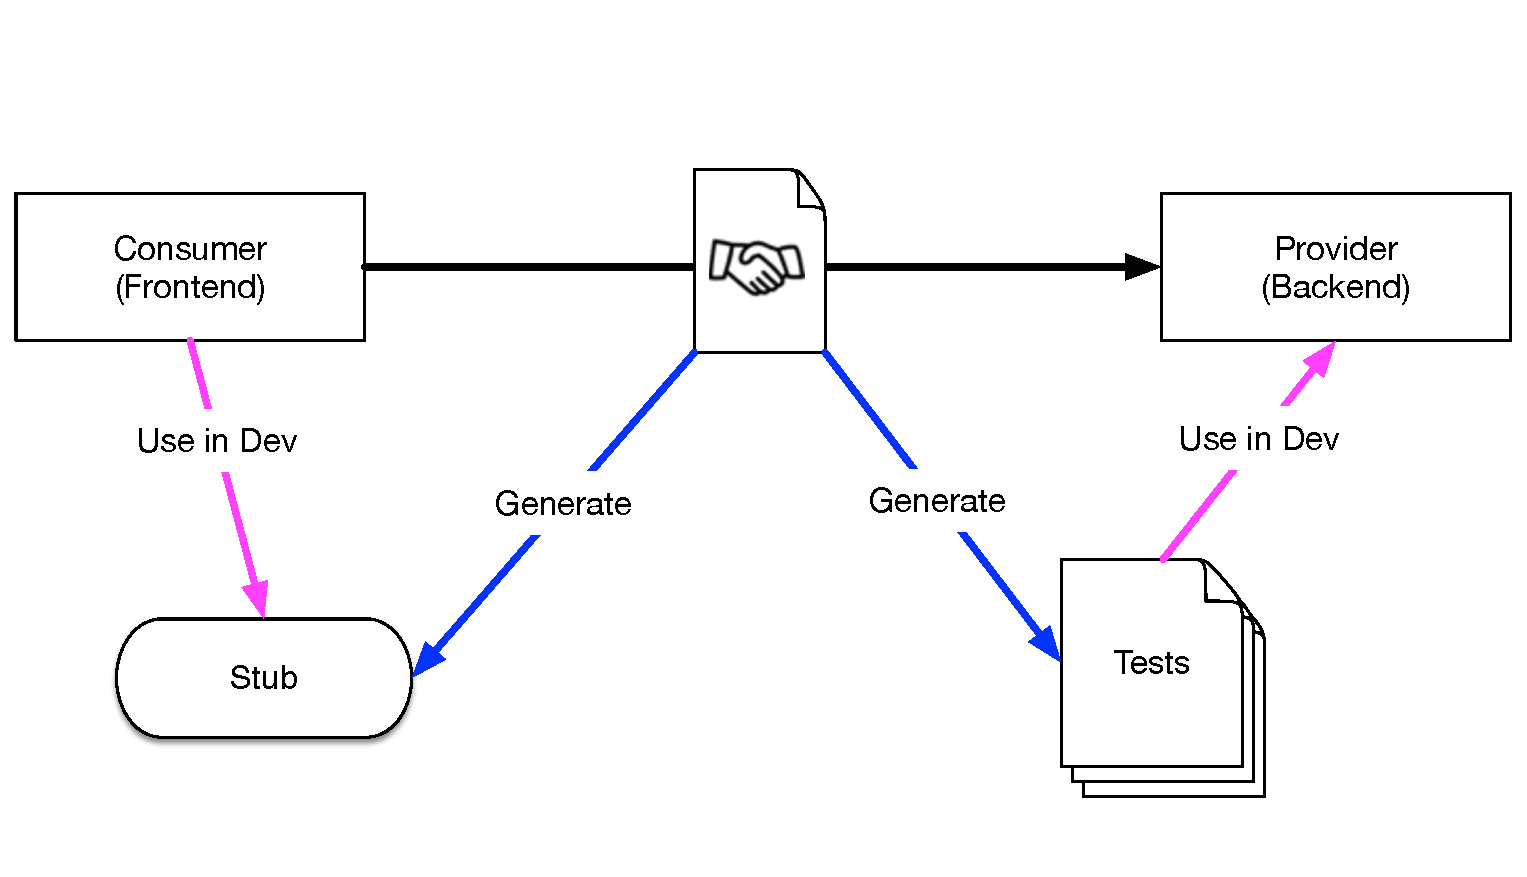
\includegraphics[width=\textwidth]{images/CDCT6.pdf}
}

\only<7>{
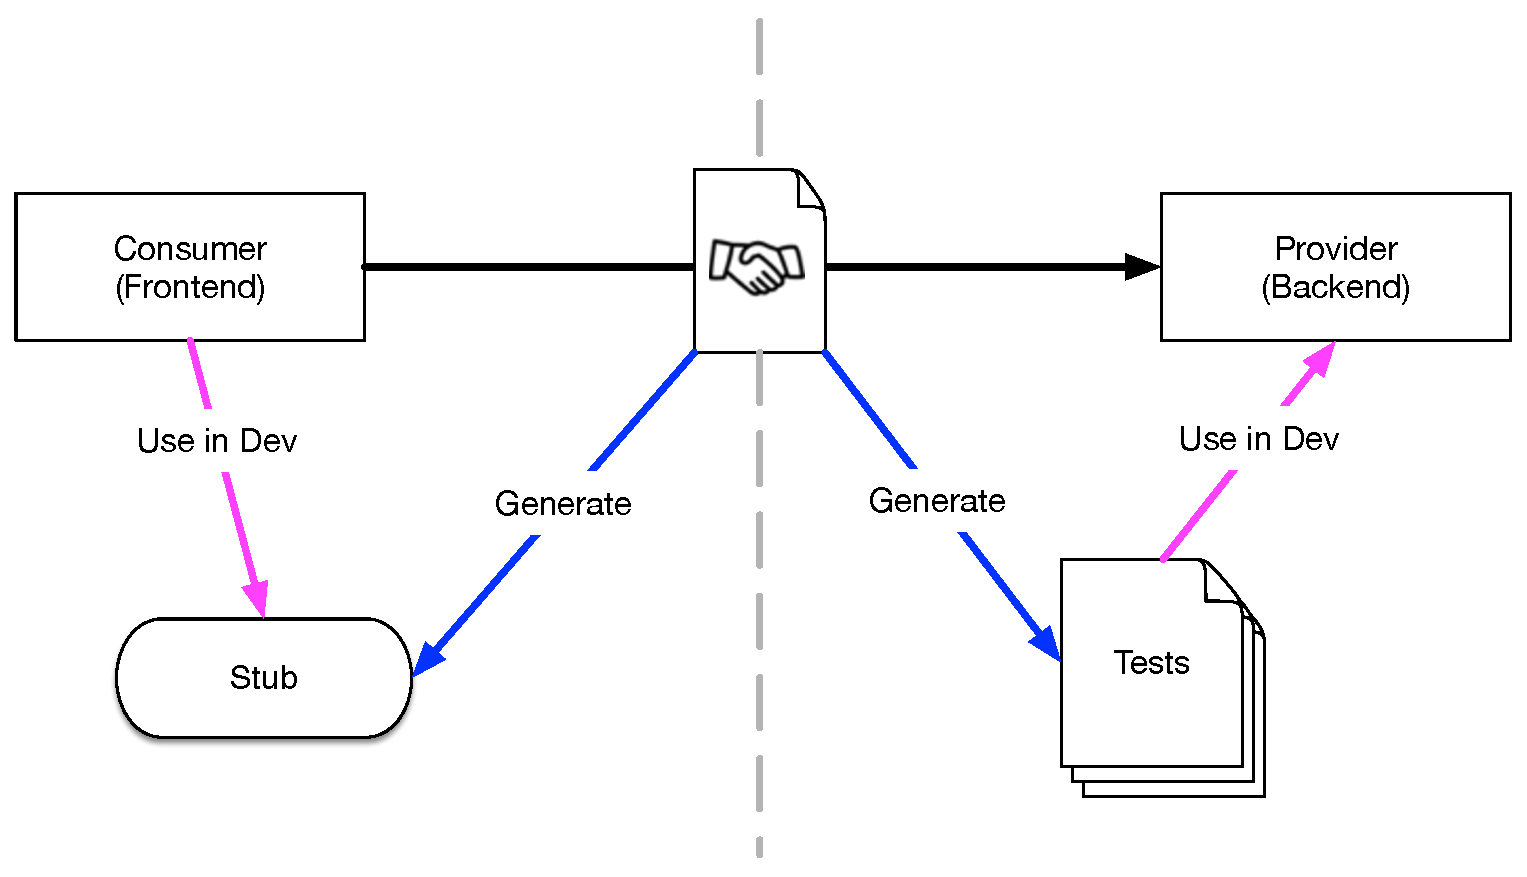
\includegraphics[width=\textwidth]{images/CDCT7.pdf}
}

\end{frame}

%%%%%%%%%%%%%%%%%%%%%%%%%%%%%%%%%%%%%%%%%%%%%%%%%%
\begin{frame}[fragile]{Example: Pet Store Domain}

\begin{itemize}
\item List all pets
\item Add pet
\item Remove pet
\end{itemize}

\end{frame}

%%%%%%%%%%%%%%%%%%%%%%%%%%%%%%%%%%%%%%%%%%%%%%%%%%
\begin{frame}[fragile]{Example: Pet Store Contracts I}

  \lstinputlisting{contracts/nopets}

\end{frame}


\begin{frame}[fragile]{Situation}

\begin{itemize}[<+->]
\item GET-Request
\item Does not depend on state
\item Easy to handle with CDCT
\end{itemize}
\end{frame}

\begin{frame}[fragile]{Questions}

\begin{itemize}[<+->]
\item Did we really document all requests (+ responses) in our contract?
\end{itemize}

\end{frame}


%%%%%%%%%%%%%%%%%%%%%%%%%%%%%%%%%%%%%%%%%%%%%%%%%%
\begin{frame}[fragile]{Example: Pet Store Contracts II}

  \lstinputlisting{contracts/somepets}

\end{frame}


\begin{frame}[fragile]{Situation}

\begin{itemize}[<+->]
\item GET-Request that depends on state
\item POST-/PUT-/DELETE-Requests
\item Difficult to handle with CDCT
\item Backend state needs to be established somehow
\item State checks need to be established somehow
\end{itemize}
\end{frame}


\begin{frame}[fragile]{Questions}

\begin{itemize}[<+->]
\item Did we really document all requests (+ responses) in our contract?
\item All possible combinations with different backend states?

\vspace{1em}
\item What are valid states in our stub?
\item Did we always establish a valid state in our stub?
\item How do we establish them (technically) before the request?
\item How do we validate them after the request?

\vspace{1em}
\item How can we keep track of our contracts and avoid redundancies?
\item How can we effectively maintain the contracts in case of changes?
\end{itemize}


\end{frame}

%%%%%%%%%%%%%%%%%%%%%%%%%%%%%%%%%%%%%%%%%%%%%%%%%%
\begin{frame}[fragile]{}

\begin{center}
{\Huge
Can Formal Methods Help??
}
\end{center}

\end{frame}

%%%%%%%%%%%%%%%%%%%%%%%%%%%%%%%%%%%%%%%%%%%%%%%%%%
\begin{frame}[fragile]{}

 \begin{tikzpicture}
 % x (kleiner = weiter nach links) y (kleiner = weiter nach unten)
%             \put (-25,-157.3) 
%{ \includegraphics[height=\paperheight]{images/boygroup.jpg} };
             \put (-55,-157.3) 
{ 
\includegraphics[height=\paperheight]{images/seraphino.jpg} };
\end{tikzpicture}

\end{frame}

%%%%%%%%%%%%%%%%%%%%%%%%%%%%%%%%%%%%%%%%%%%%%%%%%%
\begin{frame}[fragile]{}

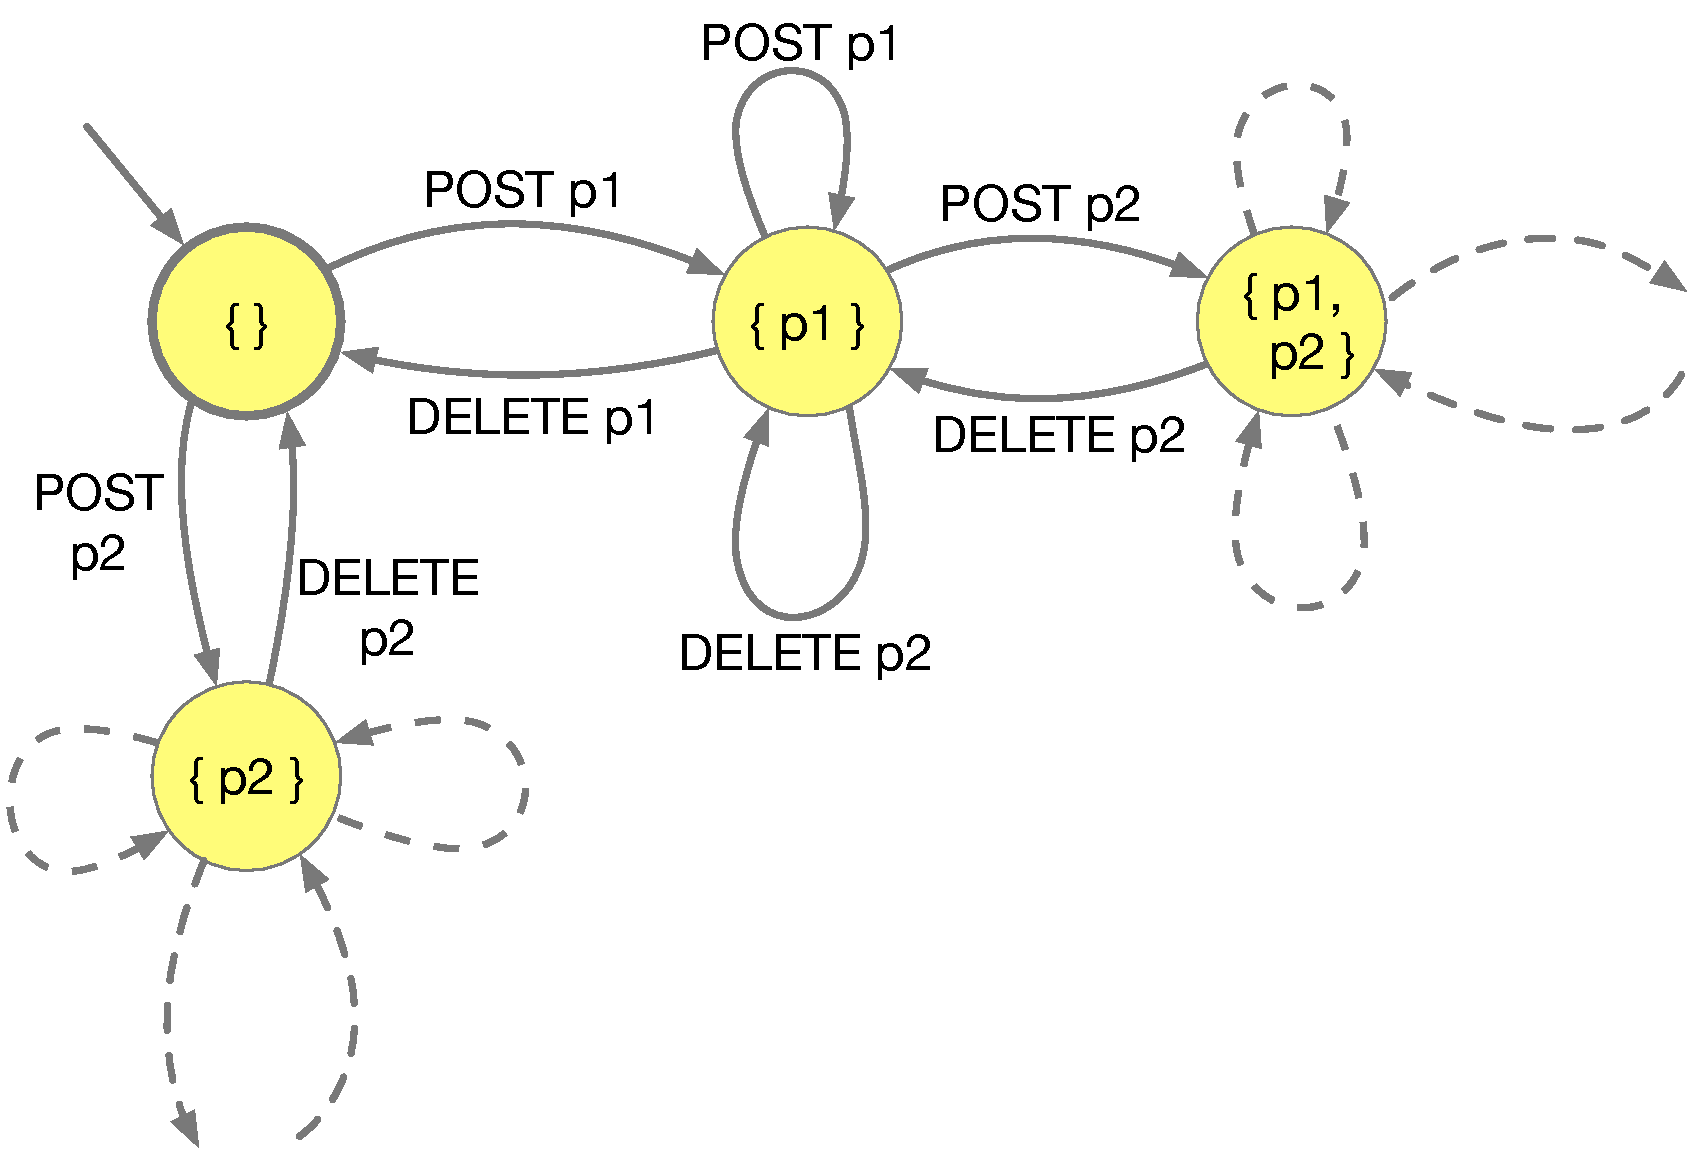
\includegraphics[width=\textwidth]{images/statemachine.pdf}

\end{frame}


%%%%%%%%%%%%%%%%%%%%%%%%%%%%%%%%%%%%%%%%%%%%%%%%%%
\begin{frame}[fragile]{}

\begin{center}
{\Huge
Sounds cool, but...

\onslide<2->
\vspace{1.5em}
... how can I build this?
}
\end{center}

\end{frame}

%%%%%%%%%%%%%%%%%%%%%%%%%%%%%%%%%%%%%%%%%%%%%%%%%%
\begin{frame}[fragile]{Building a State Machine}

\begin{itemize}
\item Implements the functionality
\item In the simplest possible way
\item In any language
\end{itemize}

\end{frame}

\begin{frame}[fragile]{The Pets Model}

\begin{lstlisting}[language=JavaScript]
class Pets {
    constructor(){
        this._pets = [];
    }

    getPets() {
        return petSorter.sortPets(this._pets);
    }

    addPet(pet) {
        this._pets.push(pet);
        return 'Pet successfully added.';
    }

    removePet(pet) {
        this._pets = this._pets.filter(
            p => p.petName !== pet.petName || p.petType !== pet.petType);
        return 'Pet successfully removed.';
    }
}
\end{lstlisting}

\end{frame}

\begin{frame}[fragile]{The Overall Model}

\begin{lstlisting}[language=Javascript]
class Model {
    constructor() {
        this._pets = new Pets();
    }

    pets() {
        return this._pets;
    }
}
\end{lstlisting}

\end{frame}

\begin{frame}[fragile]{The Model App}

\begin{lstlisting}[language=Javascript]
let model = new Model();

router.get('/pets', (req, res) => {
    const pets = model.pets().getPets();
    res.json({tag: 'Pets', pets});
});

router.post('/pets', (req, res) => {
    const message = model.pets().addPet({ petName: req.body.petName, petPrice: req.body.petPrice, petType: req.body.petType });
    res.json({message});
});

router.delete('/pets', (req, res) => {
    const message = model.pets().removePet({ petName: req.body.petName, petPrice: req.body.petPrice, petType: req.body.petType });
    res.json({message});
});
\end{lstlisting}

\end{frame}


\begin{frame}[fragile]{Important Addition}

\begin{lstlisting}[language=Javascript]
router.delete('/reset', (req, res) => {
    model = new Model();
    res.json({message: 'All pets successfully removed.'});
});
\end{lstlisting}

\end{frame}


%%%%%%%%%%%%%%%%%%%%%%%%%%%%%%%%%%%%%%%%%%%%%%%%%%
\begin{frame}[fragile]{}

\begin{center}
{\Huge
How to Use the Model?
}
\end{center}

\end{frame}


\begin{frame}[fragile]{}

\only<1>{
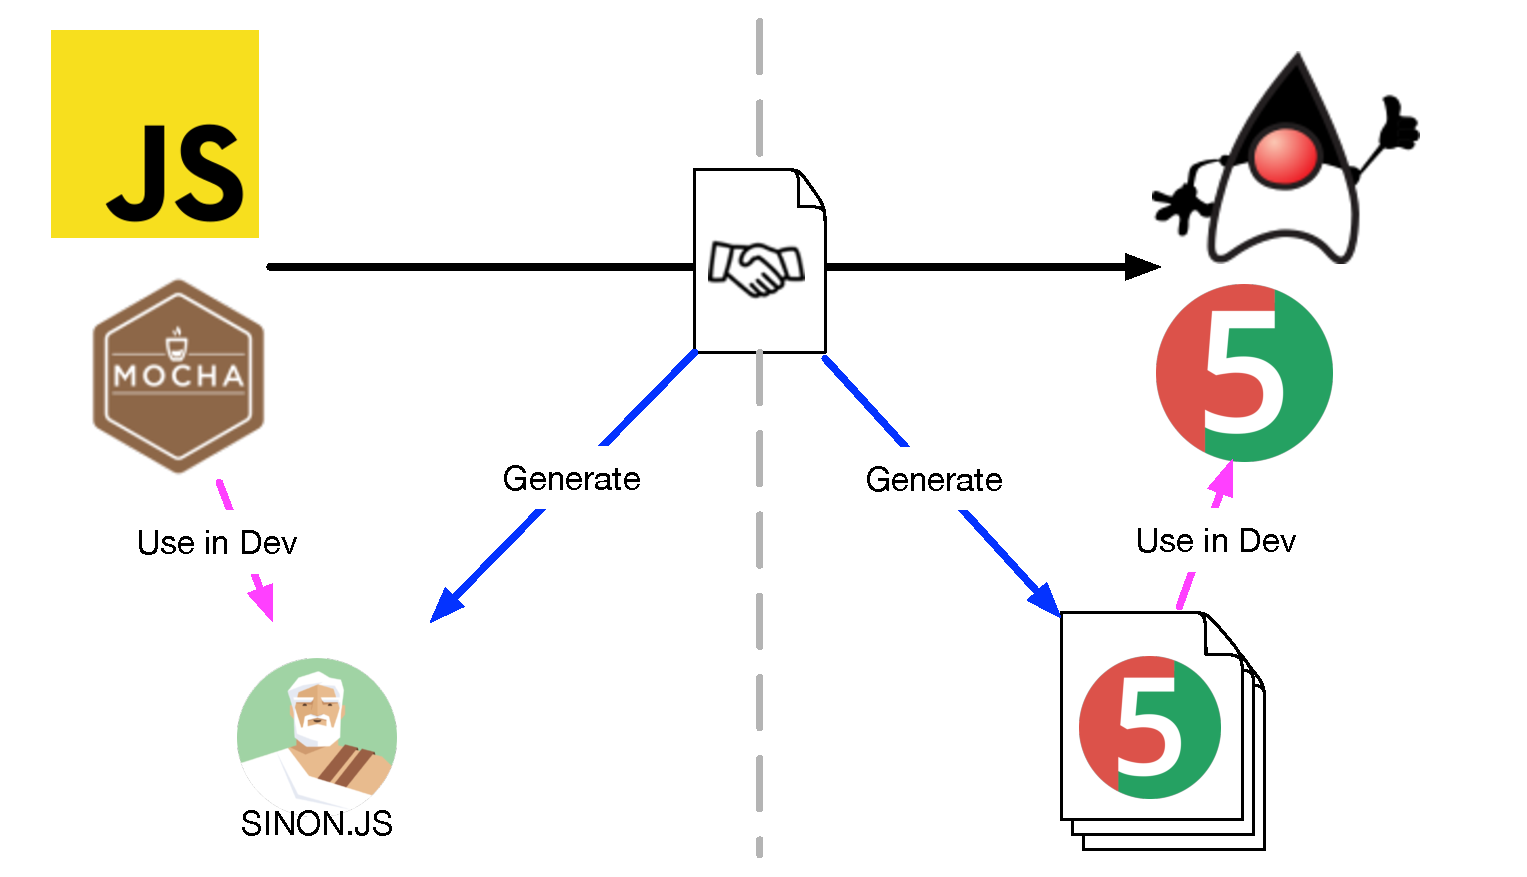
\includegraphics[width=\textwidth]{images/Model-1.pdf}
}

\only<2>{
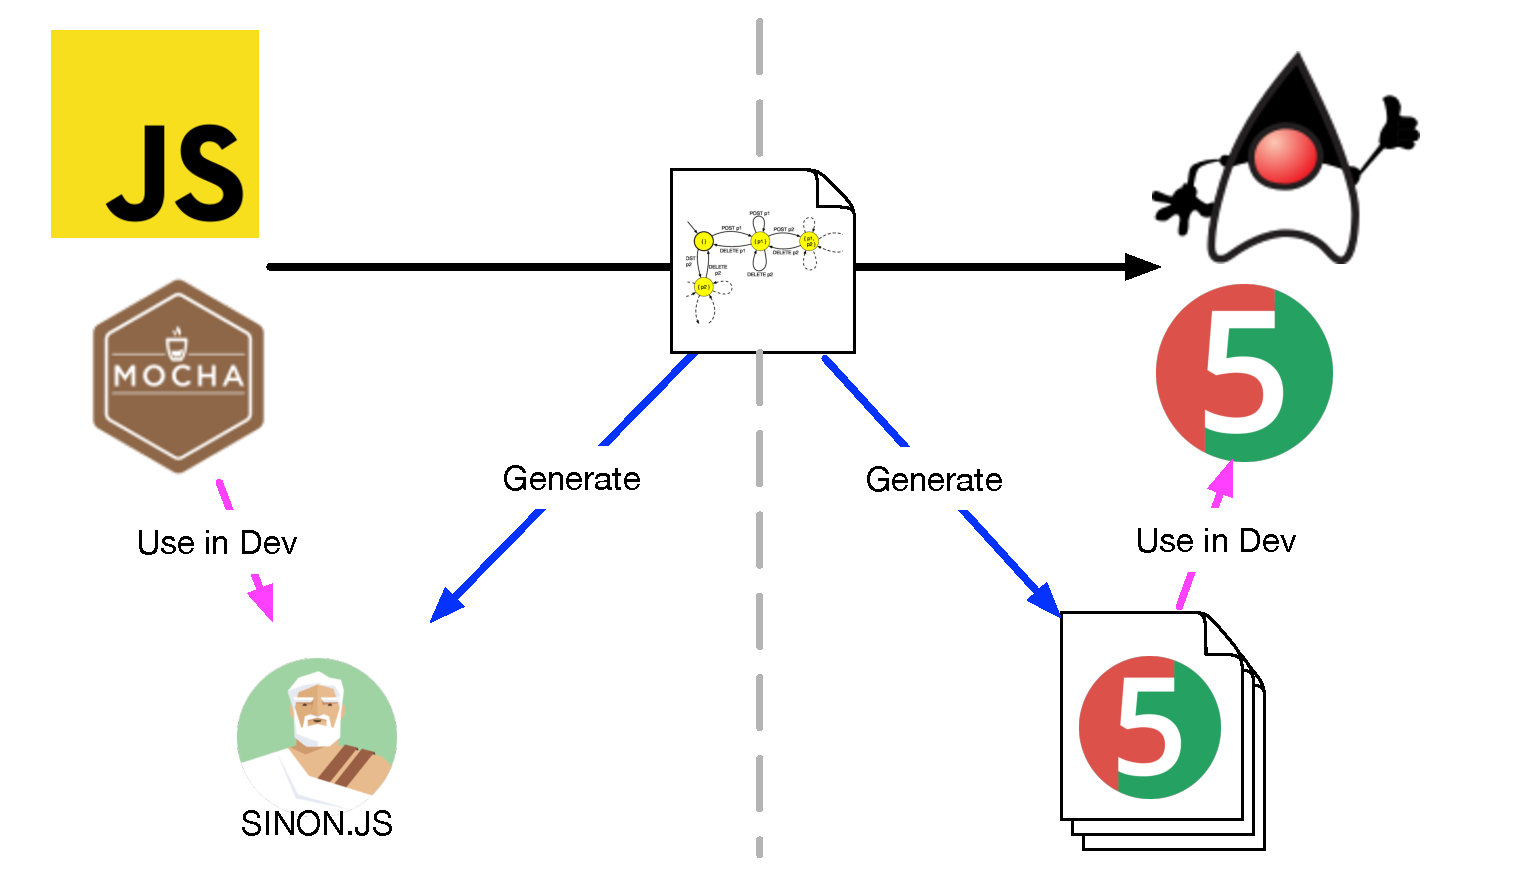
\includegraphics[width=\textwidth]{images/Model-2.pdf}
}

\only<3>{
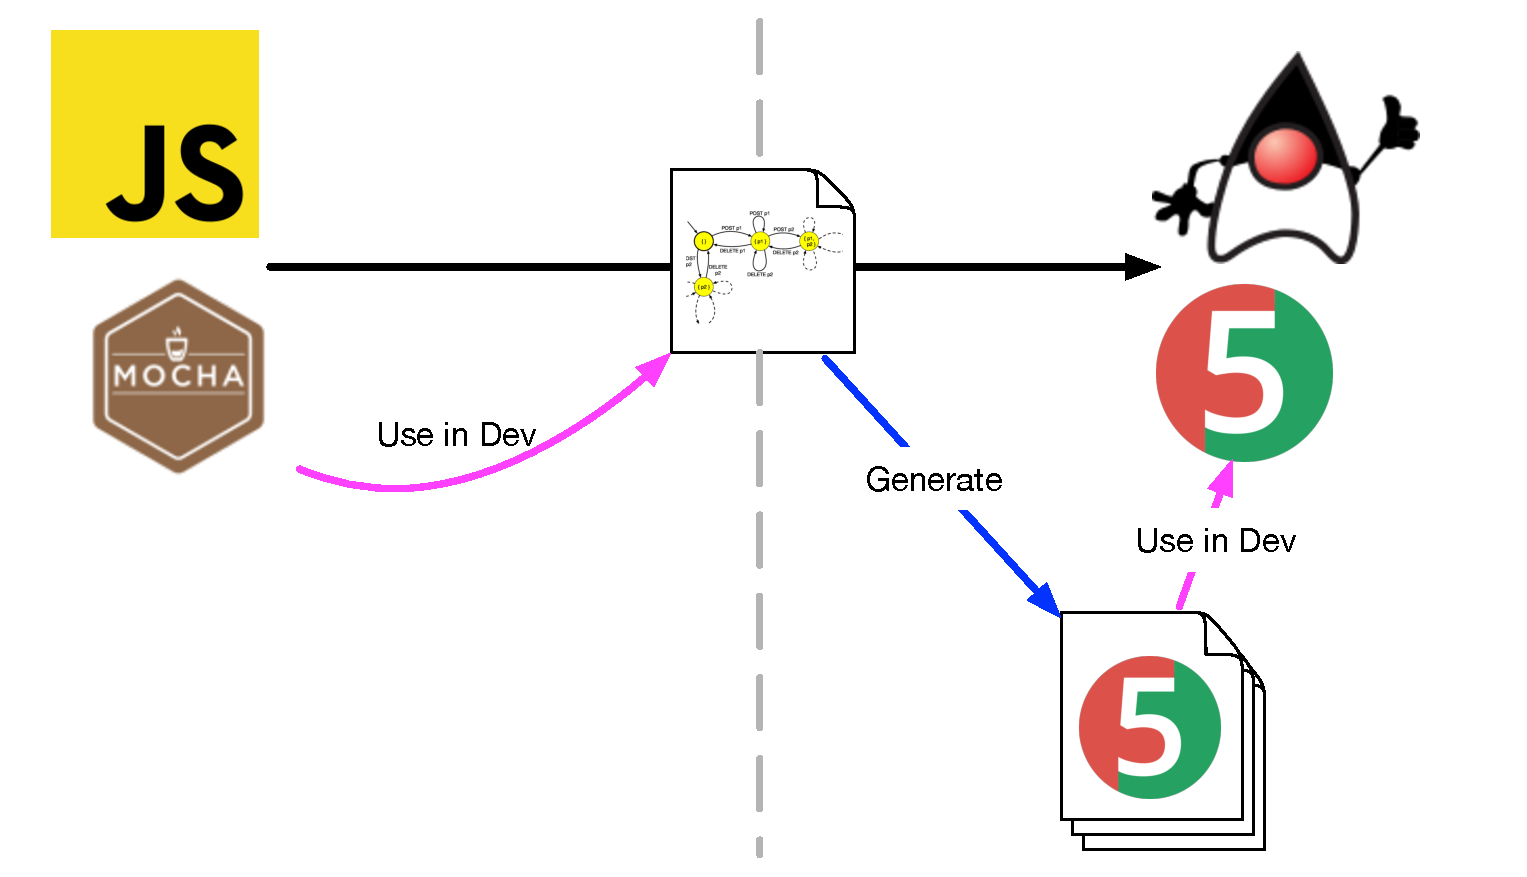
\includegraphics[width=\textwidth]{images/Model-3.pdf}
}

\only<4>{
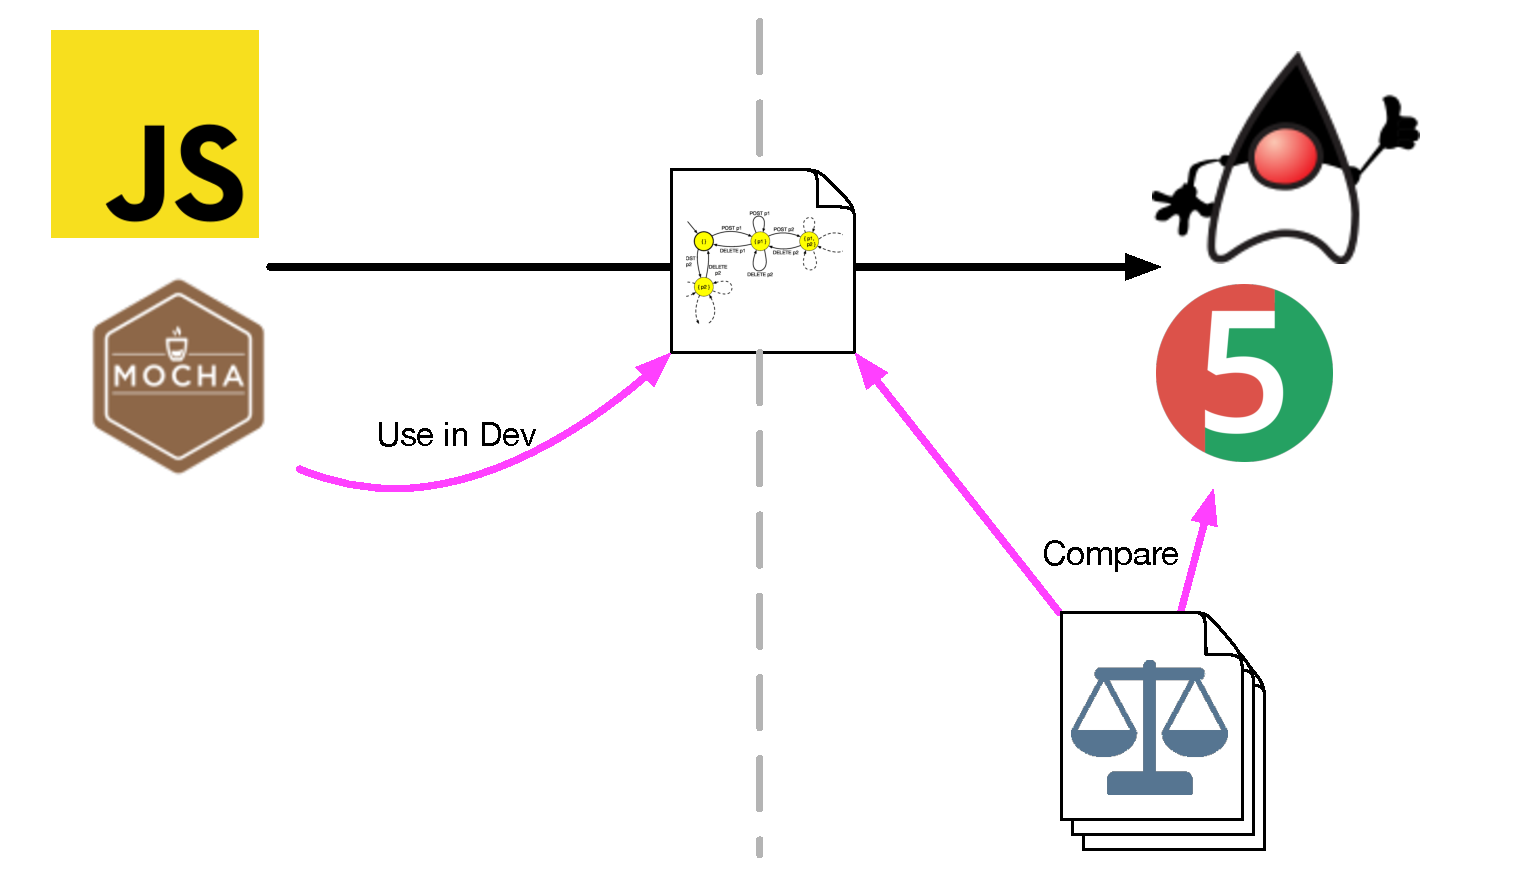
\includegraphics[width=\textwidth]{images/Model-4.pdf}
}

\end{frame}

%%%%%%%%%%%%%%%%%%%%%%%%%%%%%%%%%%%%%%%%%%%%%%%%%%
\begin{frame}[fragile]{}

\begin{center}
{\Huge
How does the Comparison work?
}
\end{center}

\end{frame}

%%%%%%%%%%%%%%%%%%%%%%%%%%%%%%%%%%%%%%%%%%%%%%%%%%
\begin{frame}[fragile]{Detour: Quick Check / Property-Based Testing}

\onslide+<2->
\begin{itemize}
\item User specifies properties
\item Tool generates examples
\item Checks properties against examples
\end{itemize}

\onslide+<3->
\begin{lstlisting}[language=Haskell]
prop_RevRev xs = reverse (reverse xs) == xs
  where types = xs::[Int]
\end{lstlisting}

\onslide+<4->
\begin{lstlisting}
Main> quickCheck prop_RevRev
OK, passed 100 tests.
\end{lstlisting}

\onslide+<5->
\begin{lstlisting}
prop_RevId xs = reverse xs == xs
  where types = xs::[Int]
\end{lstlisting}

\onslide+<6->
\begin{lstlisting}
Main> quickCheck prop_RevId
Falsifiable, after 1 tests:
[-3,15]
\end{lstlisting}

\end{frame}


%%%%%%%%%%%%%%%%%%%%%%%%%%%%%%%%%%%%%%%%%%%%%%%%%%
%%%%%%%%%%%%%%%%%%%%%%%%%%%%%%%%%%%%%%%%%%%%%%%%%%
%%%%%%%%%%%%%%%%%%%%%%%%%%%%%%%%%%%%%%%%%%%%%%%%%%

langsam auseinanderbauen, grafisch aufzeigen


\begin{frame}[fragile]{The Problems with CDCT}

\begin{itemize}[<+->]
\item Provider testing must manually establish the desired state
\item Contract testing is only as good as its contracts
\item Manual contract-writing can be tedious and even error-prone
\item Errors may only be discovered late in the process, when the backend implements some functionality and discovers that it does not match the contract
\item If contracts are too sparse, we miss out
\item If contracts are too verbose (or too many), testing takes too long
- Contract maintenance

\item What if some request only makes sense in a certain state?
\end{itemize}

\end{frame}

%%%%%%%%%%%%%%%%%%%%%%%%%%%%%%%%%%%%%%%%%%%%%%%%%%
\part{Beyond CDCT}

\begin{frame}[fragile]{Back to Formal Language}
  \begin{itemize}[<+->]
  \item Often contracts are fairly simple, just mapping requests to replies
  \item What if some request only makes sense in a certain state?
  \item We need more information: Let's use \emph{State Machines}!
  \end{itemize}
\end{frame}


\begin{frame}[fragile]{Our ``formal model'' approach}

  \begin{itemize}[<+->]
  \item Describe the core domain interactions as a formally verifiable model
  \item Generate mocks for the frontend: Use the State Machine as an \emph{Acceptor}
  \item Generate tests for the backend: Use the State Machine as a \emph{Generator}
  \item Guarantee: All aspects of  the model are covered by tests and mocks
  \end{itemize}

\end{frame}

\begin{frame}[fragile]{Model-Based Interaction Testing}
  \only<1>{
    \begin{center}
      \includegraphics[height=.8\textheight]{./images/modelling-interaction-1.pdf}
    \end{center}
  }
  \only<2>{
    \begin{center}
      \includegraphics[height=.8\textheight]{./images/modelling-interaction-2.pdf}
    \end{center}
  }
  \only<3>{
    \begin{center}
      \includegraphics[height=.8\textheight]{./images/modelling-interaction-3.pdf}
    \end{center}
  }
  \only<4>{
    \begin{center}
      \includegraphics[height=.8\textheight]{./images/modelling-interaction-4.pdf}
    \end{center}
  }
  \only<5>{
    \begin{center}
      \includegraphics[height=.8\textheight]{./images/modelling-interaction-5.pdf}
    \end{center}
  }
\end{frame}



\begin{frame}[fragile]{Example: PetStore Model}
\begin{lstlisting}[language=Haskell,basicstyle=\ttfamily,keywordstyle=\color{red}]
petStore :: Input
         -> PetStore
         -> (Maybe Output, PetStore)

petStore Add{pet}  store@PetStore{storedPets}
  | pet `notElem` storedPets =
      (Just $ PetAdded pet,
       store { storedPets = pet:storedPets } )

  | otherwise                =
      (Just $ Error PetAlreadyAdded, store)
\end{lstlisting}
\end{frame}

\begin{frame}[fragile]{Demo}
  \begin{center}
    \Huge{Validating the backend \& frontend}
  \end{center}
\end{frame}

\begin{frame}[fragile]{Demo}
  \begin{center}
    \Huge{Updating the model}
  \end{center}
\end{frame}

\begin{frame}[fragile]{Real World Application}
  \begin{itemize}[<+->]
  \item Testing Implementation of a Smart Contracts transaction scheduling platform
  \item Define a Model of the system in terms of \emph{Actions}, observable \emph{State} and potential \emph{Failures} from components
  \item Generate sequence of \emph{Action}
  \item Run \emph{Actions} in parallel against the Model and the Implementation
  \item Check reached states in Implementation is identical to the Model's
  \end{itemize}
\end{frame}


%%%%%%%%%%%%%%%%%%%%%%%%%%%%%%%%%%%%%%%%%%%%%%%%%%
\part{Conclusion}

\begin{frame}[fragile]{Event Sourcing \& Formal Methods}
  \begin{itemize}[<+->]
  \item Building an\emph{Event Sourced} system yields opportunities to leverage more formal approaches to Verification \& Validation
  \item Modelling as a \emph{State Machine} over a \emph{Formal Language} seems a promising approach
  \item Provides foundations to develop independent parts of the system and \emph{validate} their interaction
  \item It takes time and energy to devise and refine a model!
  \end{itemize}
\end{frame}

\begin{frame}[fragile]{Takeaways}
  \only<1>{\Huge \begin{quote} Plans are worthless,\\ but planning is everything \\ \textsc{\Large Dwight D. Eisenhower}\end{quote}}
  \only<2>{\Huge \begin{quote} Models are worthless,\\ but modelling is everything \\ \textsc{\Large Nicole \& Arnaud}\end{quote}}
\end{frame}

%%%%%%%%%%%%%%%%%%%%%%%%%%%%%%%%%%%%%%%%%%%%%%%%%%
\begin{frame}{Thank you very much!}

  ~\\[1em]
  \begin{block}{Nicole Rauch}
    \begin{description}[Twitterxx]
    \item[E-Mail]  \href{mailto:info@nicole-rauch.de}{\texttt{info@nicole-rauch.de}}
    \item[Twitter] \href{http://twitter.com/NicoleRauch}{\texttt{@NicoleRauch}}
    \item[Web] \href{http://www.nicole-rauch.de}{\texttt{http://www.nicole-rauch.de}}
    \end{description}
  \end{block}
\end{frame}


%%%%%%%%%%%%%%%%%%%%%%%%%%%%%%%%%%%%%%%%%%%%%%%%%%
\begin{frame}{Credits}

Models: Eva Rinaldi - Myer Spring Summer Fashion Launch \\
{\footnotesize \url{https://www.flickr.com/photos/evarinaldiphotography/6032441835}}


{\footnotesize \url{}}
{\footnotesize \url{}}
{\footnotesize \url{}}

\end{frame}
